
\section{Introduction}

ECAL performance is crucial for precision measurements that involve electrons and photons. 
(Higgs decaying to two photons). Also, for the reconstruction of the jets and missing transverse energies (as mentioned PF section).

(reminder from CMS section) ECAL is designed to measure the energy deposited by electrons and photons. These particles deposit their energy in ECAL by showering in the ECAL crystals. (next describe EM showers here briefly)

EM showers spread over multiple crystals. (small Molière radius 2.19 cm while crystal transverse size is close 2.6 cm). clusters are extended in phi direction to form "superclusters" to recover energy radiated via bremsstrahlung or conversion. (connect with PF section)

To get the correct energy for a photon we generally include corrections that was done before data taking (Intercalibration: equalize signal response for the same eta, Laser corrections for signal transparency loss (or photocathode aging) this calibration is done every 40 mins) and other in situ. (include equation related to calibration) cluster correction obtained from a regression method. this is thesis is focused on. (this part could move to cluster calibration section).

The reconstructed PF cluster energy is expected to be smaller than the energy of the incoming particle. This loss of energy could be due to tracker material, gaps, dead channels etc. Therefore, a calibration of the calorimeter cluster energy is needed.

This chapter presents the used ML method BDT and datasets in performing the PF ECAL cluster calibration (online/offline).  


\section{XGBoost}

(will be added soon)

\section{Datasets description}

The first part of the thesis focuses on the calibration of ECAL pf clusters.The dataset samples used in this calibration are double photon with no material samples that were available through Data Aggregation System (DAS) web page.   
They are centrally produced with 133X %(CMSSW_13_3)
conditions, Run3 Winter24 Monte Carlo (MC), and in format of a MiniAOD. They corresponding to center of mass energy 13.6 TeV with pt range up to 1500.  


\section{PF ECAL cluster regression}

The ML method implemented for PF ECAL cluster calibration is a Boosted Decision Tree (BDT) based semi-parametric regression. (technical details of XGBOOST is mentioned in ML section).

To estimate the correction to the PF ECAL Cluster, we consider the case where a one photon has deposited all its energy in one PF cluster in the ECAL. (Clusters are mentioned in PF section). This will allow us to calculate: the correction factor = E “gen photon” / E “raw pf cluster”.

% generally how the energy cluster regression is done 
The PF cluster regression is done intro two steps:  
1) Training (from where we will get trained regression model). % what ML model is mentioned in ML section.  
2) The testing of the training is done on NOPU and PU (80) samples. % mention testing of ML model in ML section. % Also PU when in dataset section.  

% specific details of the training related to the anaylsis 
Training details:Training is done on no PU Zero material double photon particle gun. During training we are going to adopt the same variables used in Run 2 calibration for Run 3 (2024). 

The training input variables include independent variables (features) used in the training:  clusrawE, ieta,iphi (EB), ix, iy (EE), ietamod20, iphimod20 (EB only), (clusPS1+clusPS2)/clusrawE (EE only) number of hits in the cluster (which takes values 1, 2 and 3 - it takes 3 if nhits >= 3).
used Target: log (Egen/Eraw). % refer to  features & target details in ML  

Training conditions (Sample): Trained for zero-suppressed and full readout regions separately.
(For full readout, three regressions are trained:raw pt [5, 20], [20, 100], and [100, 300] GeV) 
%Total of 8 regressions were trained. (Check the different types of regression model used).

The validation is done through few steps:First from the training model we get the value of the correction factor,then calculate: the corrected cluster energy = E “raw pf cluster” * correction factor 
Plot: the response: E “corrected PF cluster”/E “gen photon”. Fit the plot with: double CB function.(for pt< 6 GeV we use Gaus function for fitting since it will be difficult to do the with double CB- in other words low pt (zero suppressed))From the fitted curve we find: mean, effective sigma. We can also get the mean, effective sigma for raw PF cluster energy “with no correction” to compare. 

\section{results}

The presented plots show a comparison between the calibration results of the new (presented) corrected ECAL cluster in 133X (blue line), to the current (previous) correction in 126X (green) and raw PF ECAL cluster (red). (what has changed between the new and previous correction? Just the sample conditions? Which affected the model used in the training?)  

generally, we see that the new correction very close to the current used calibration. Usually, the since the PF clustering is performed separately in each region (this is mentioned in PF section) of the ECAL: ECAL Barrel (EB), ECAL Endcaps (EE). calibrations is done in a similar way.

Overview of the results: we checked the 2024 double photon calibration samples for PF ECAL clusters. In general, the existing calibration derived from 2022 samples seems to continue to be working well. (note: add comment about future calibration for ECAL PF cluster)


\subsection{offline PF ECAL cluster}

%\subsubsection{ECAL Barrel}
first starting with the NOPU sample then the PU case. in ECAL Barrel region. 

plots show response (resolution) vs Pt gen in GeV and in their corresponding eta range.
\begin{figure}
\includegraphics[width=0.495\textwidth]{./plots_pdf/ECAL_plots/plotsPU/EB/FULL/pdf/GENPT/EBFULL_GENPT_0005_0020_MuOverBins.pdf}
\includegraphics[width=0.495\textwidth]{./plots_pdf/ECAL_plots/plotsPU/EB/FULL/pdf/GENPT/EBFULL_GENPT_0005_0020_EffSigmaOverBins.pdf}
%\caption{EB - Full Readout pt 5-20}
%\end{figure}
%\begin{figure}
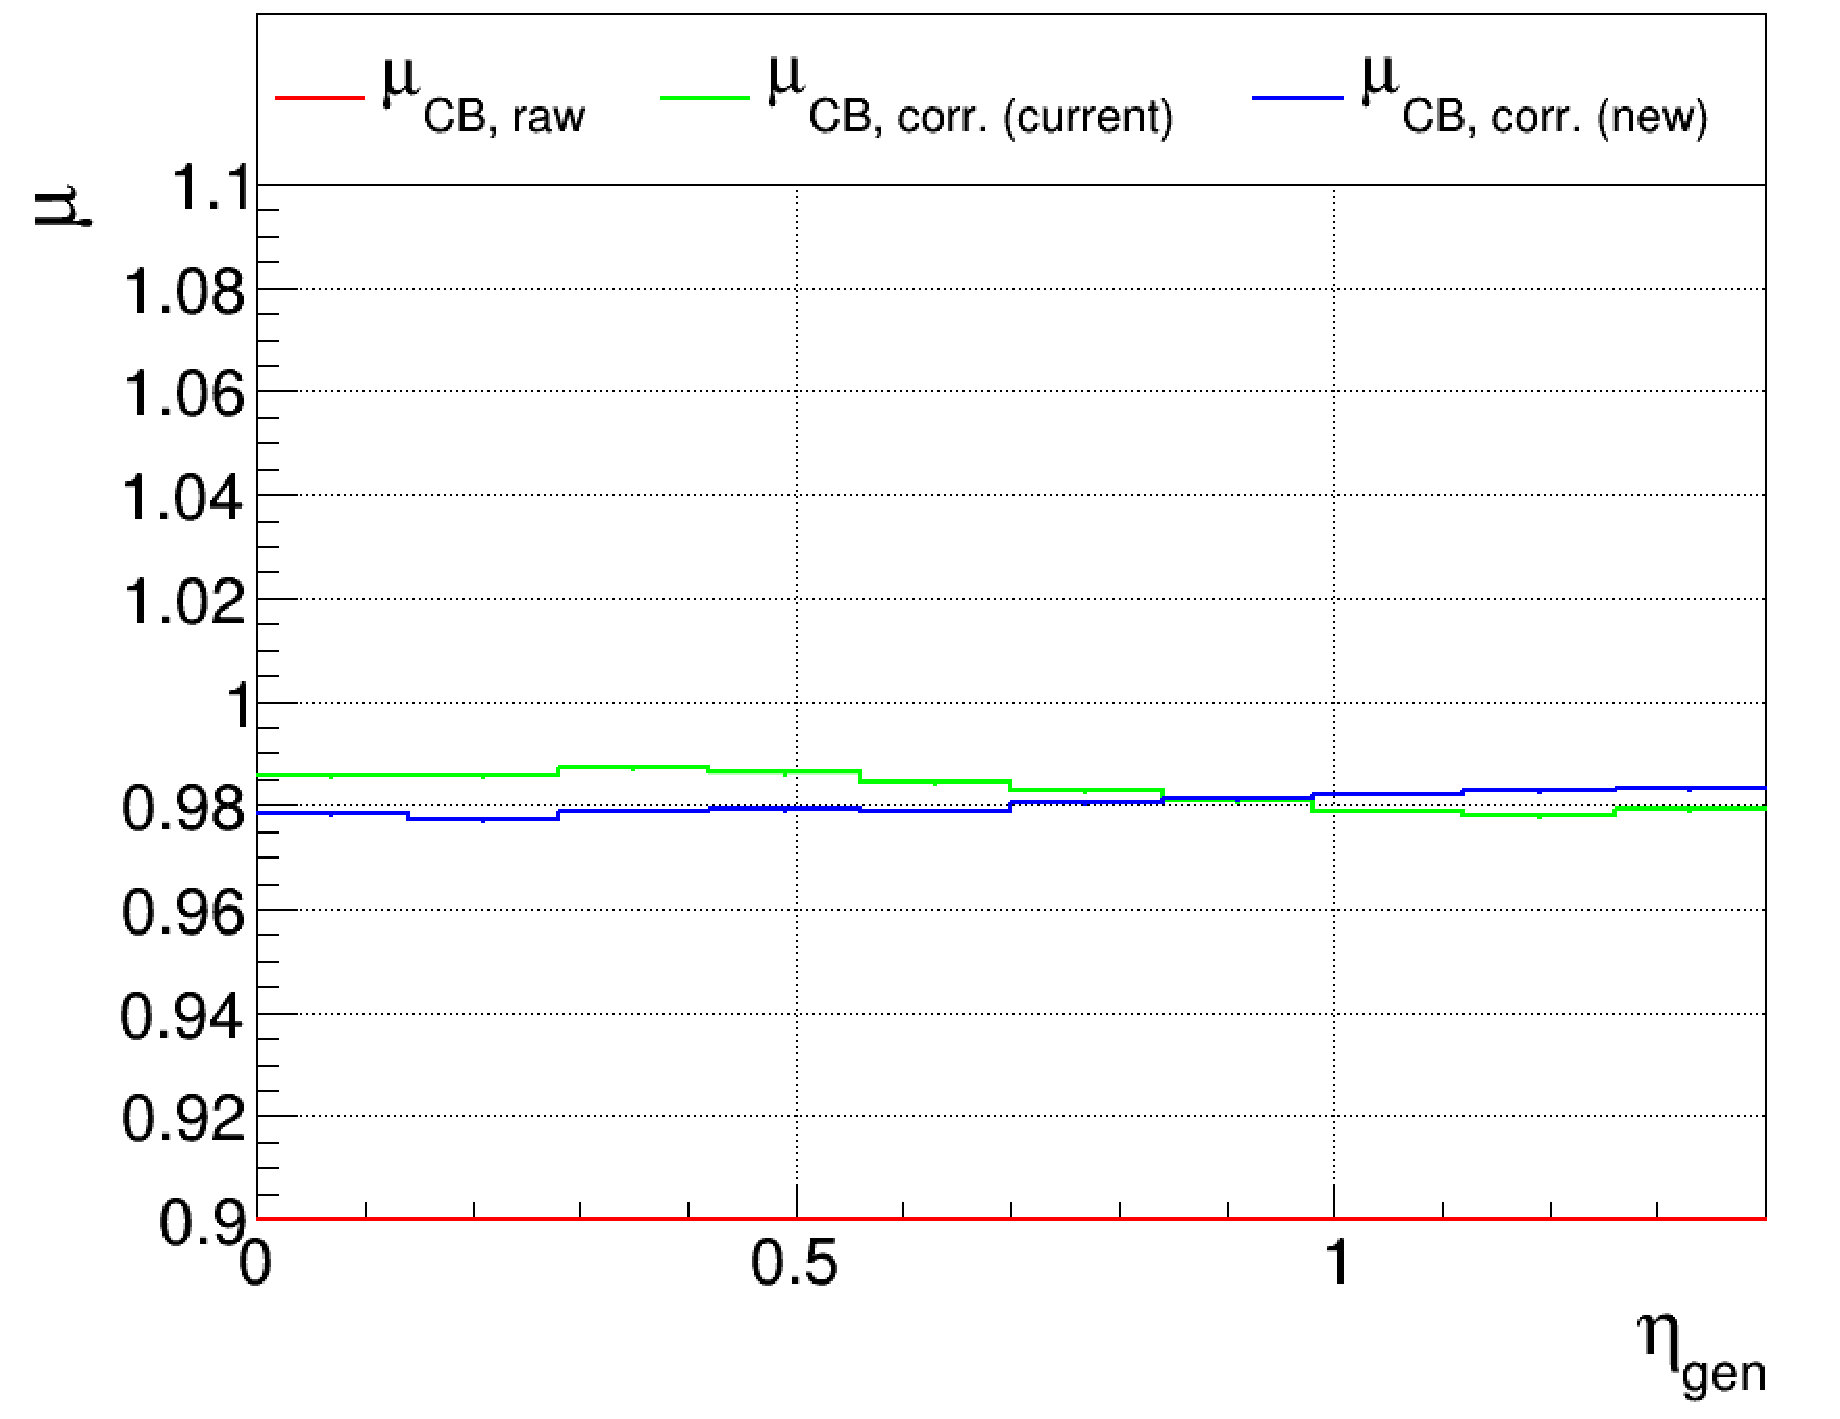
\includegraphics[width=0.495\textwidth]{./plots_pdf/ECAL_plots/plotsPU/EB/FULL/pdf/GENETA/EBFULL_GENETA_0005_0020_MuOverBins.pdf}
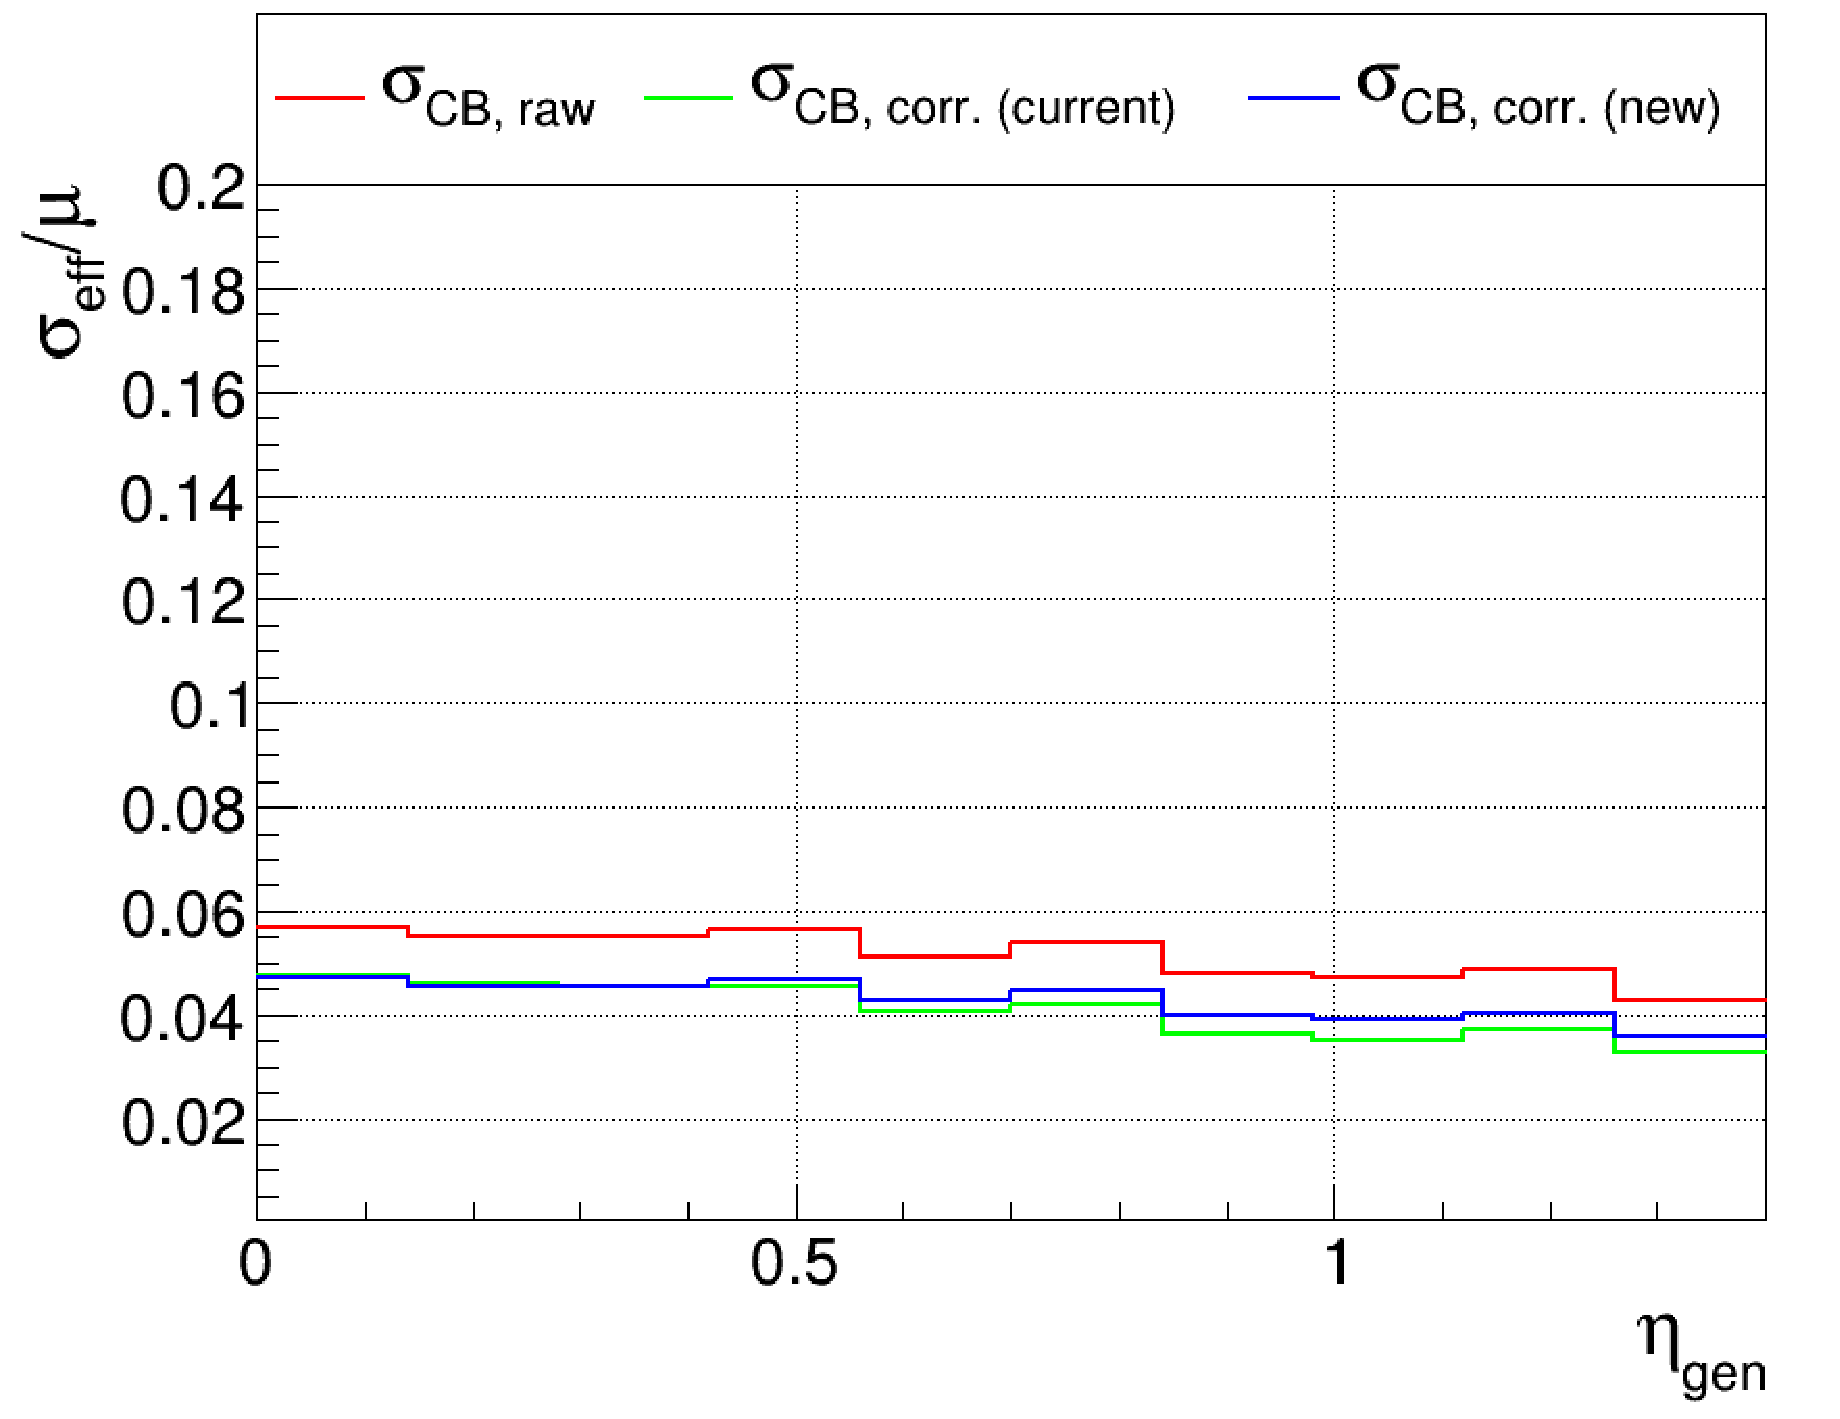
\includegraphics[width=0.495\textwidth]{./plots_pdf/ECAL_plots/plotsPU/EB/FULL/pdf/GENETA/EBFULL_GENETA_0005_0020_EffSigmaOverBins.pdf}
\caption{EB - Full Readout \pt 5--20\GeV.}
\end{figure}


\begin{figure}
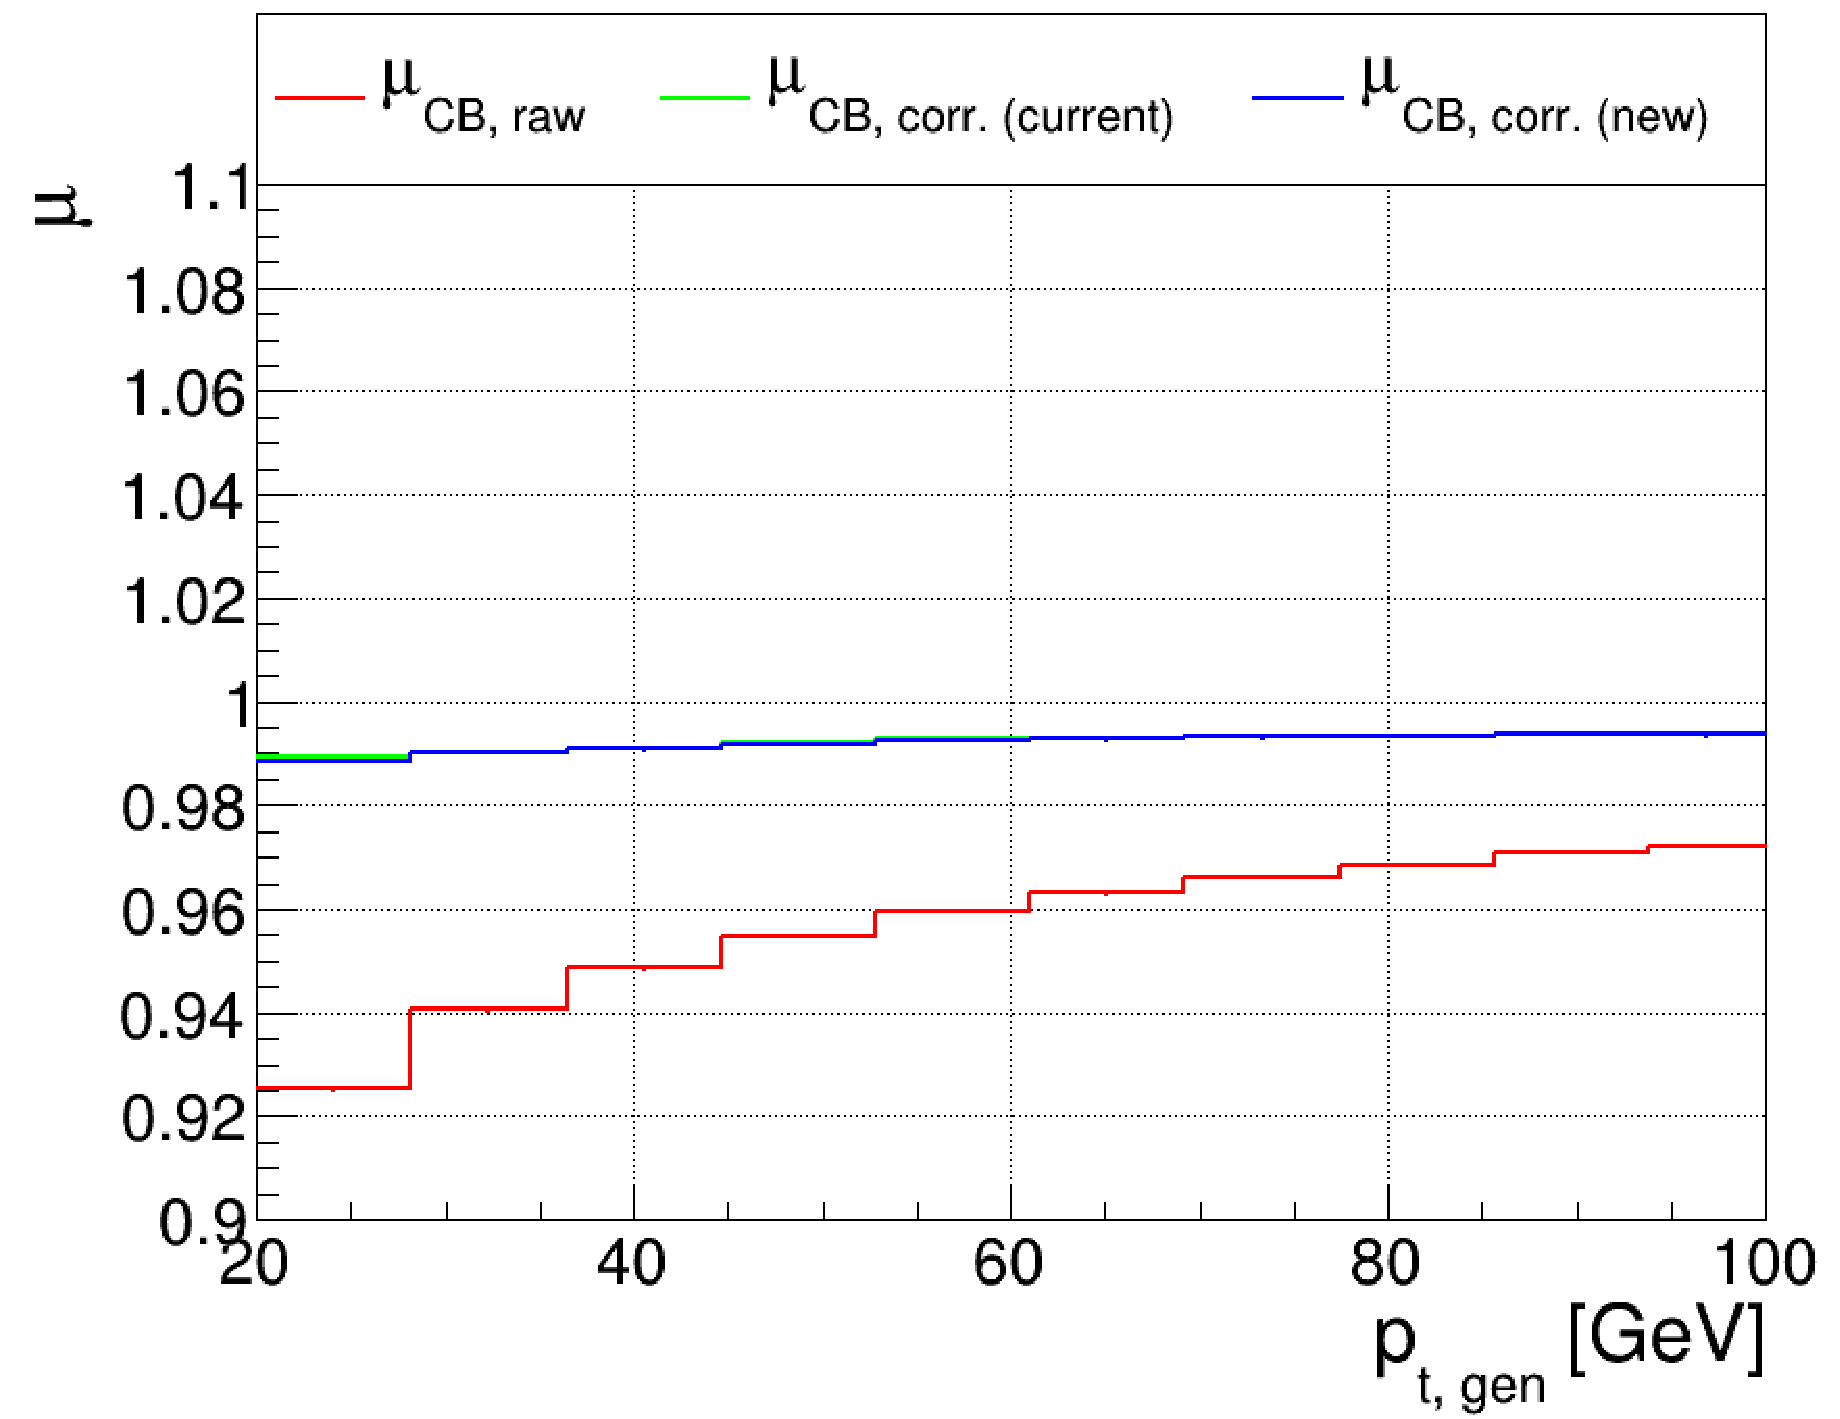
\includegraphics[width=0.495\textwidth]{./plots_pdf/ECAL_plots/plotsPU/EB/FULL/pdf/GENPT/EBFULL_GENPT_0020_0100_MuOverBins.pdf}
\includegraphics[width=0.495\textwidth]{./plots_pdf/ECAL_plots/plotsPU/EB/FULL/pdf/GENPT/EBFULL_GENPT_0020_0100_EffSigmaOverBins.pdf}
%\caption{EB - Full Readout pt 20-100}
%\end{figure}
%\begin{figure}
\includegraphics[width=0.495\textwidth]{./plots_pdf/ECAL_plots/plotsPU/EB/FULL/pdf/GENETA/EBFULL_GENETA_0020_0100_MuOverBins.pdf}
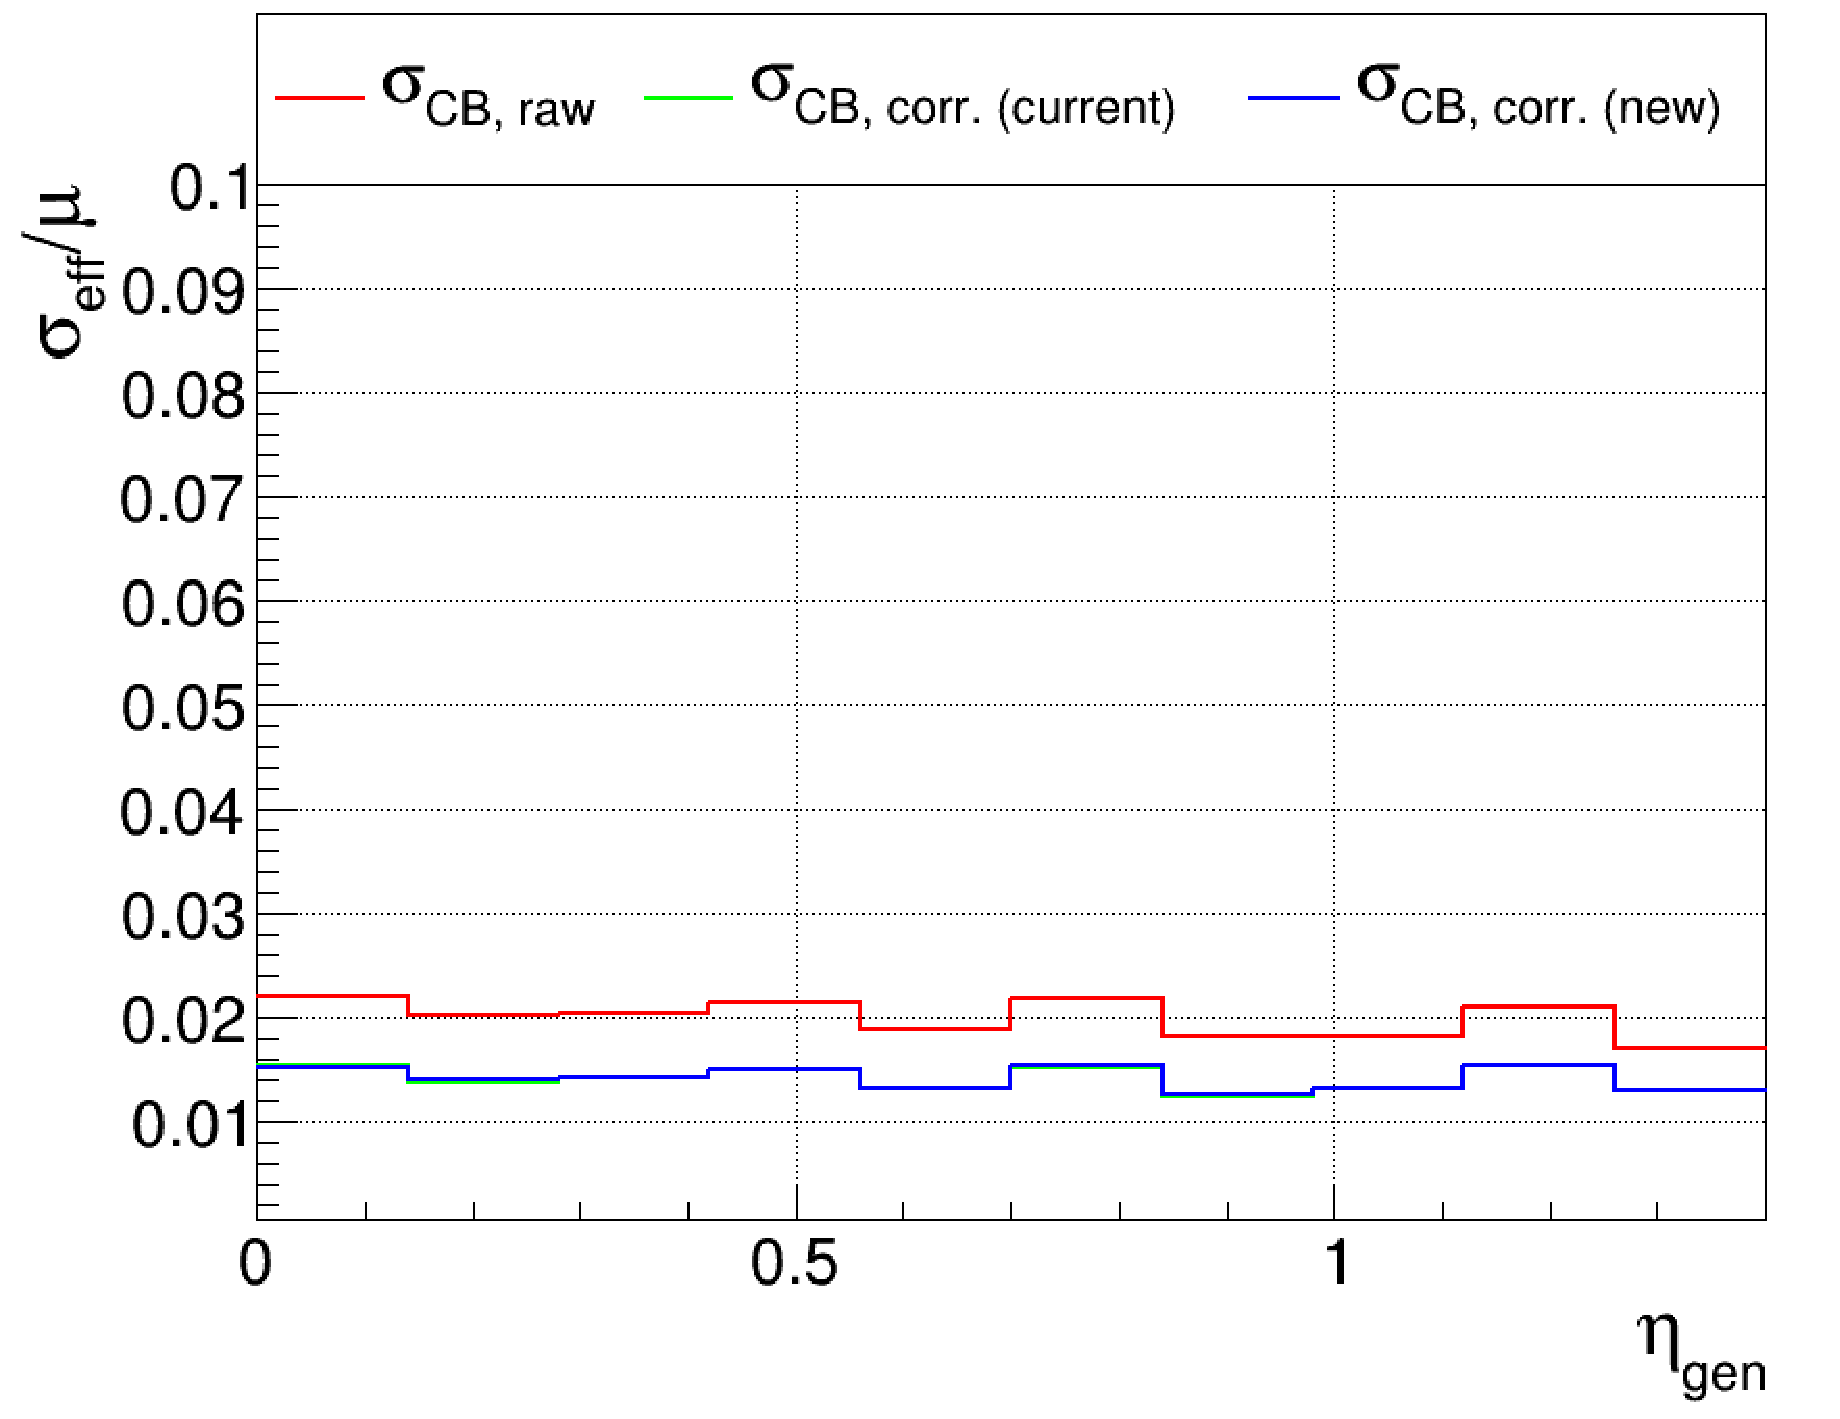
\includegraphics[width=0.495\textwidth]{./plots_pdf/ECAL_plots/plotsPU/EB/FULL/pdf/GENETA/EBFULL_GENETA_0020_0100_EffSigmaOverBins.pdf}
\caption{EB - Full Readout \pt 20--100\GeV.}
\end{figure}

\begin{figure}
\includegraphics[width=0.495\textwidth]{./plots_pdf/ECAL_plots/plotsPU/EB/FULL/pdf/GENPT/EBFULL_GENPT_0100_0300_MuOverBins.pdf}
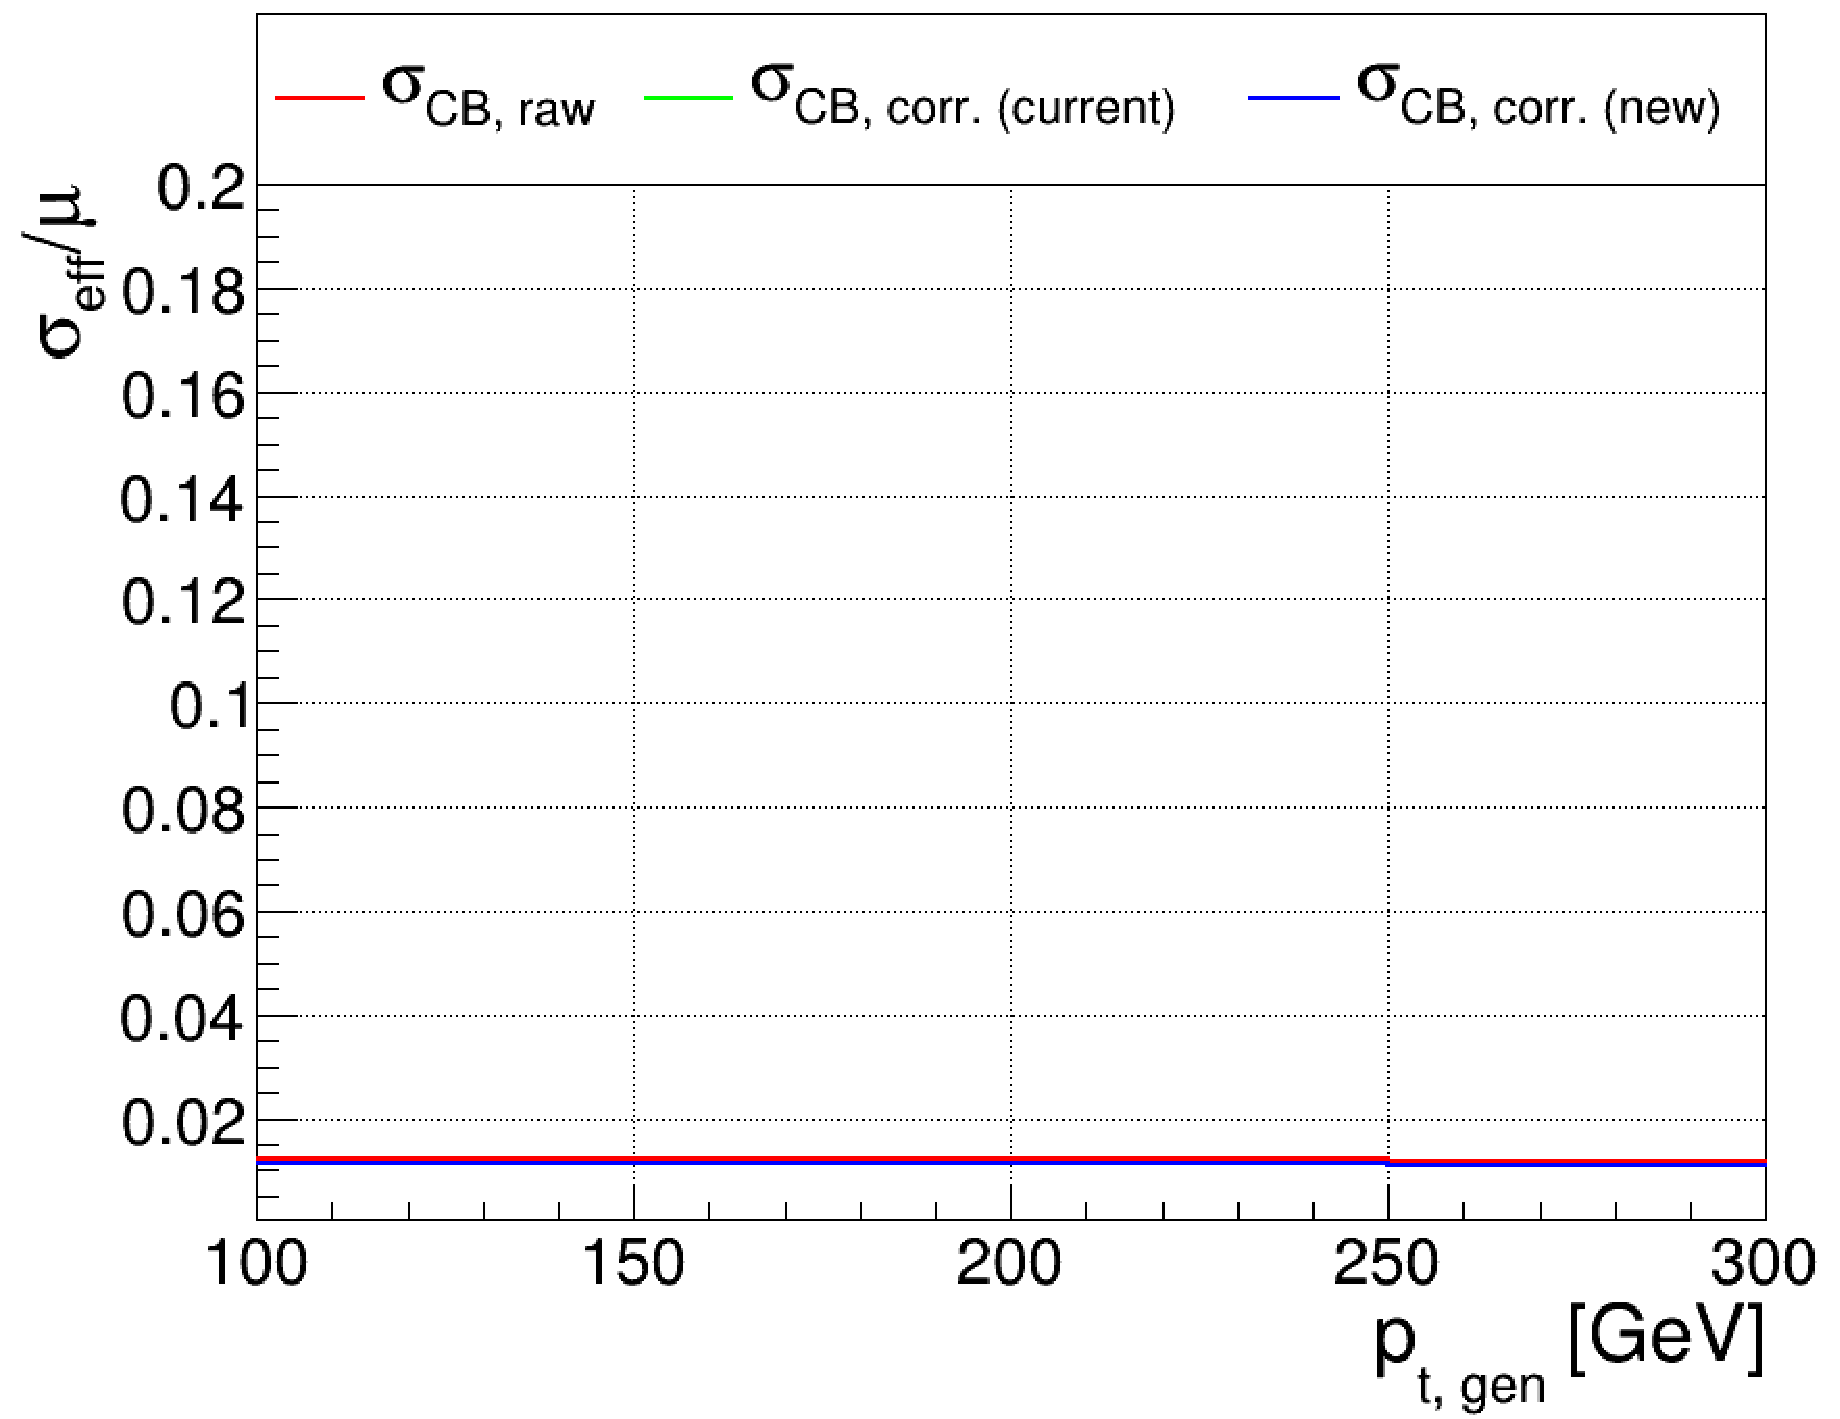
\includegraphics[width=0.495\textwidth]{./plots_pdf/ECAL_plots/plotsPU/EB/FULL/pdf/GENPT/EBFULL_GENPT_0100_0300_EffSigmaOverBins.pdf}
%\caption{EB - Full Readout pt 100-300}
%\end{figure}
%\begin{figure}
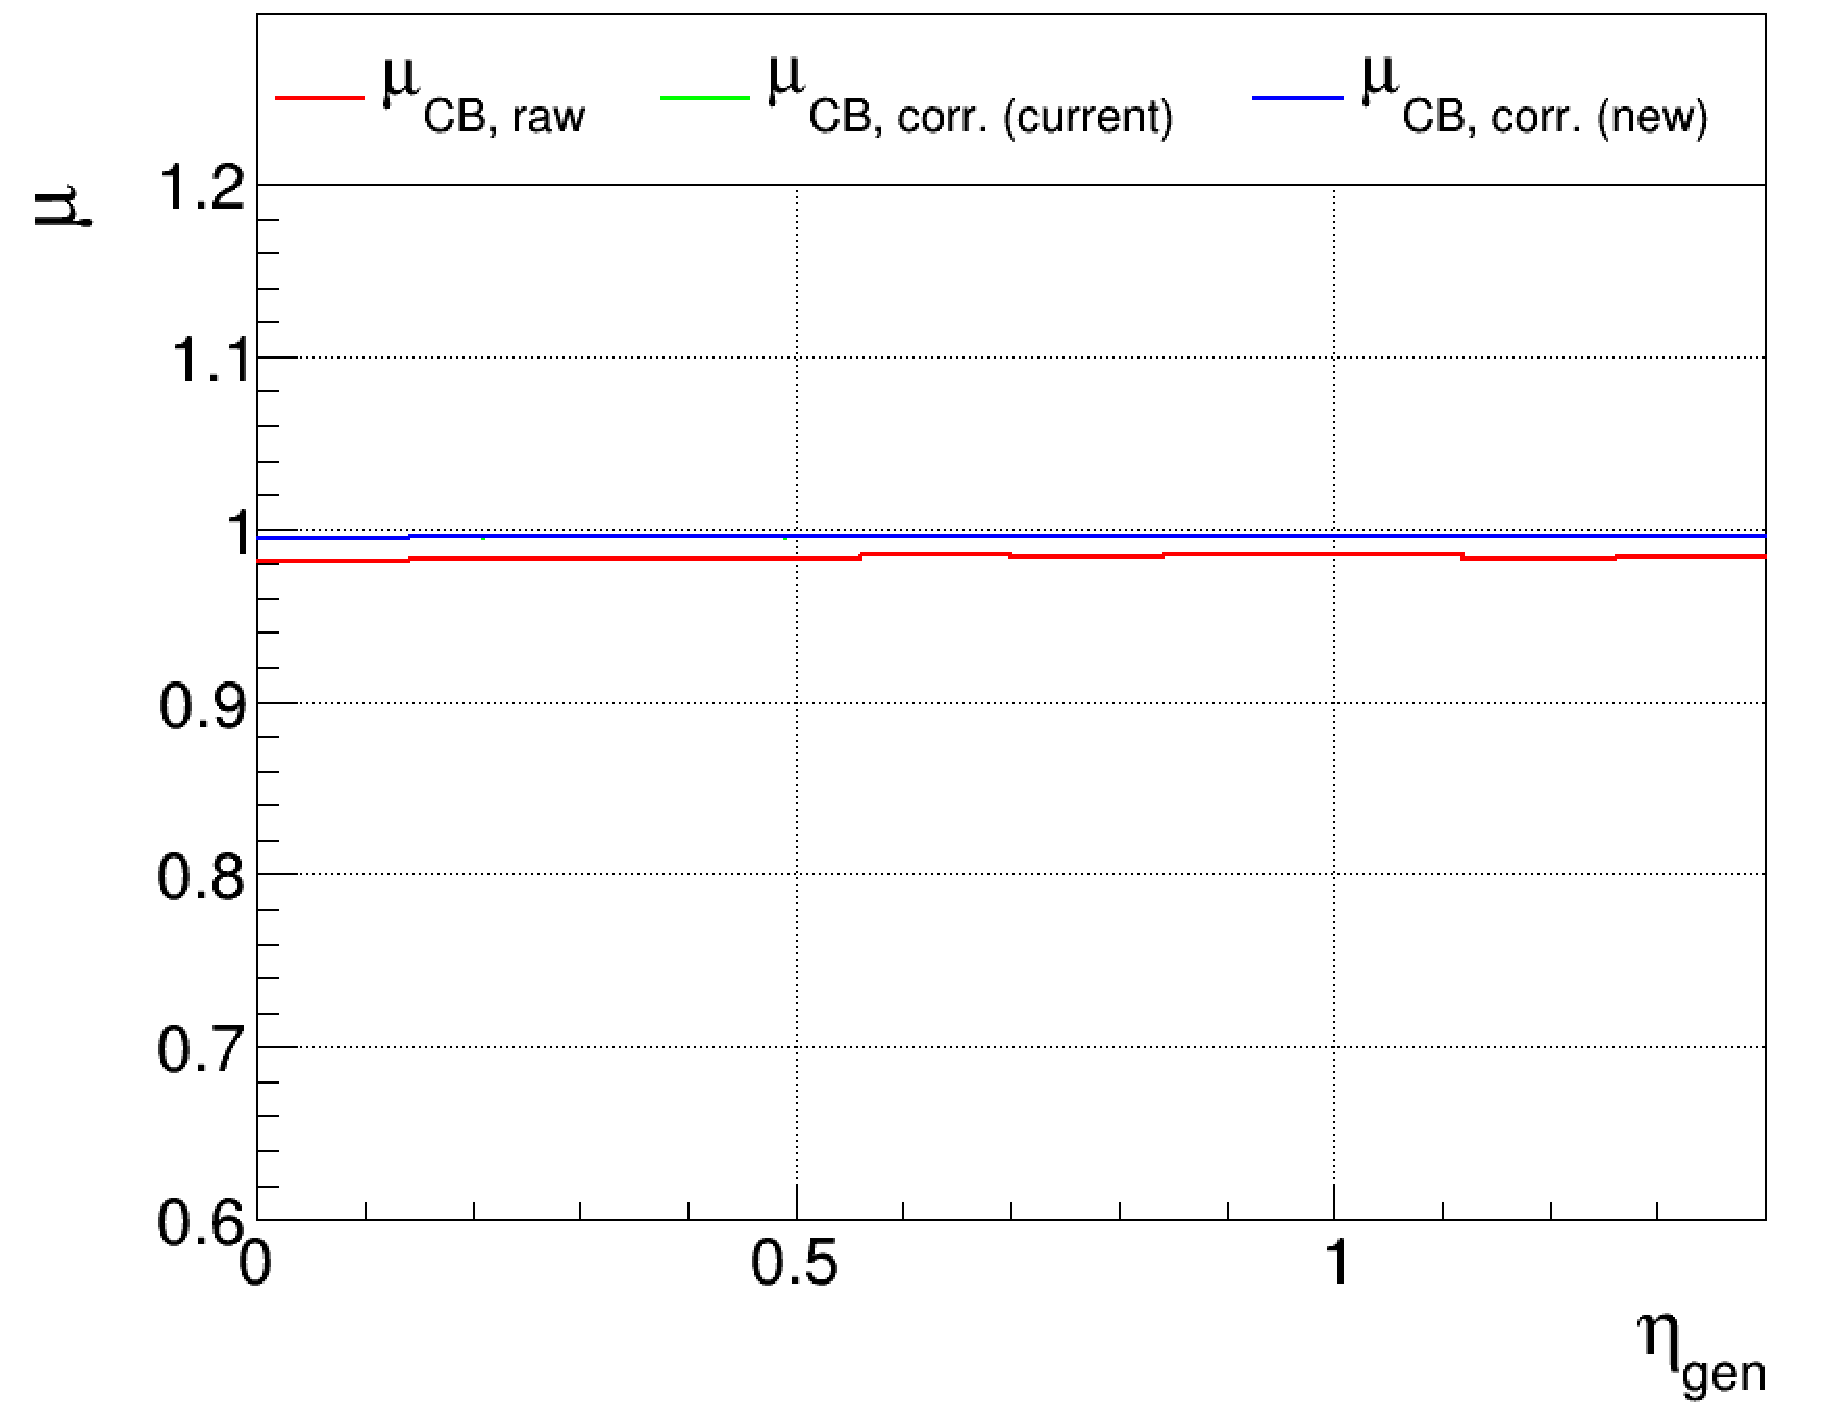
\includegraphics[width=0.495\textwidth]{./plots_pdf/ECAL_plots/plotsPU/EB/FULL/pdf/GENETA/EBFULL_GENETA_0100_0300_MuOverBins.pdf}
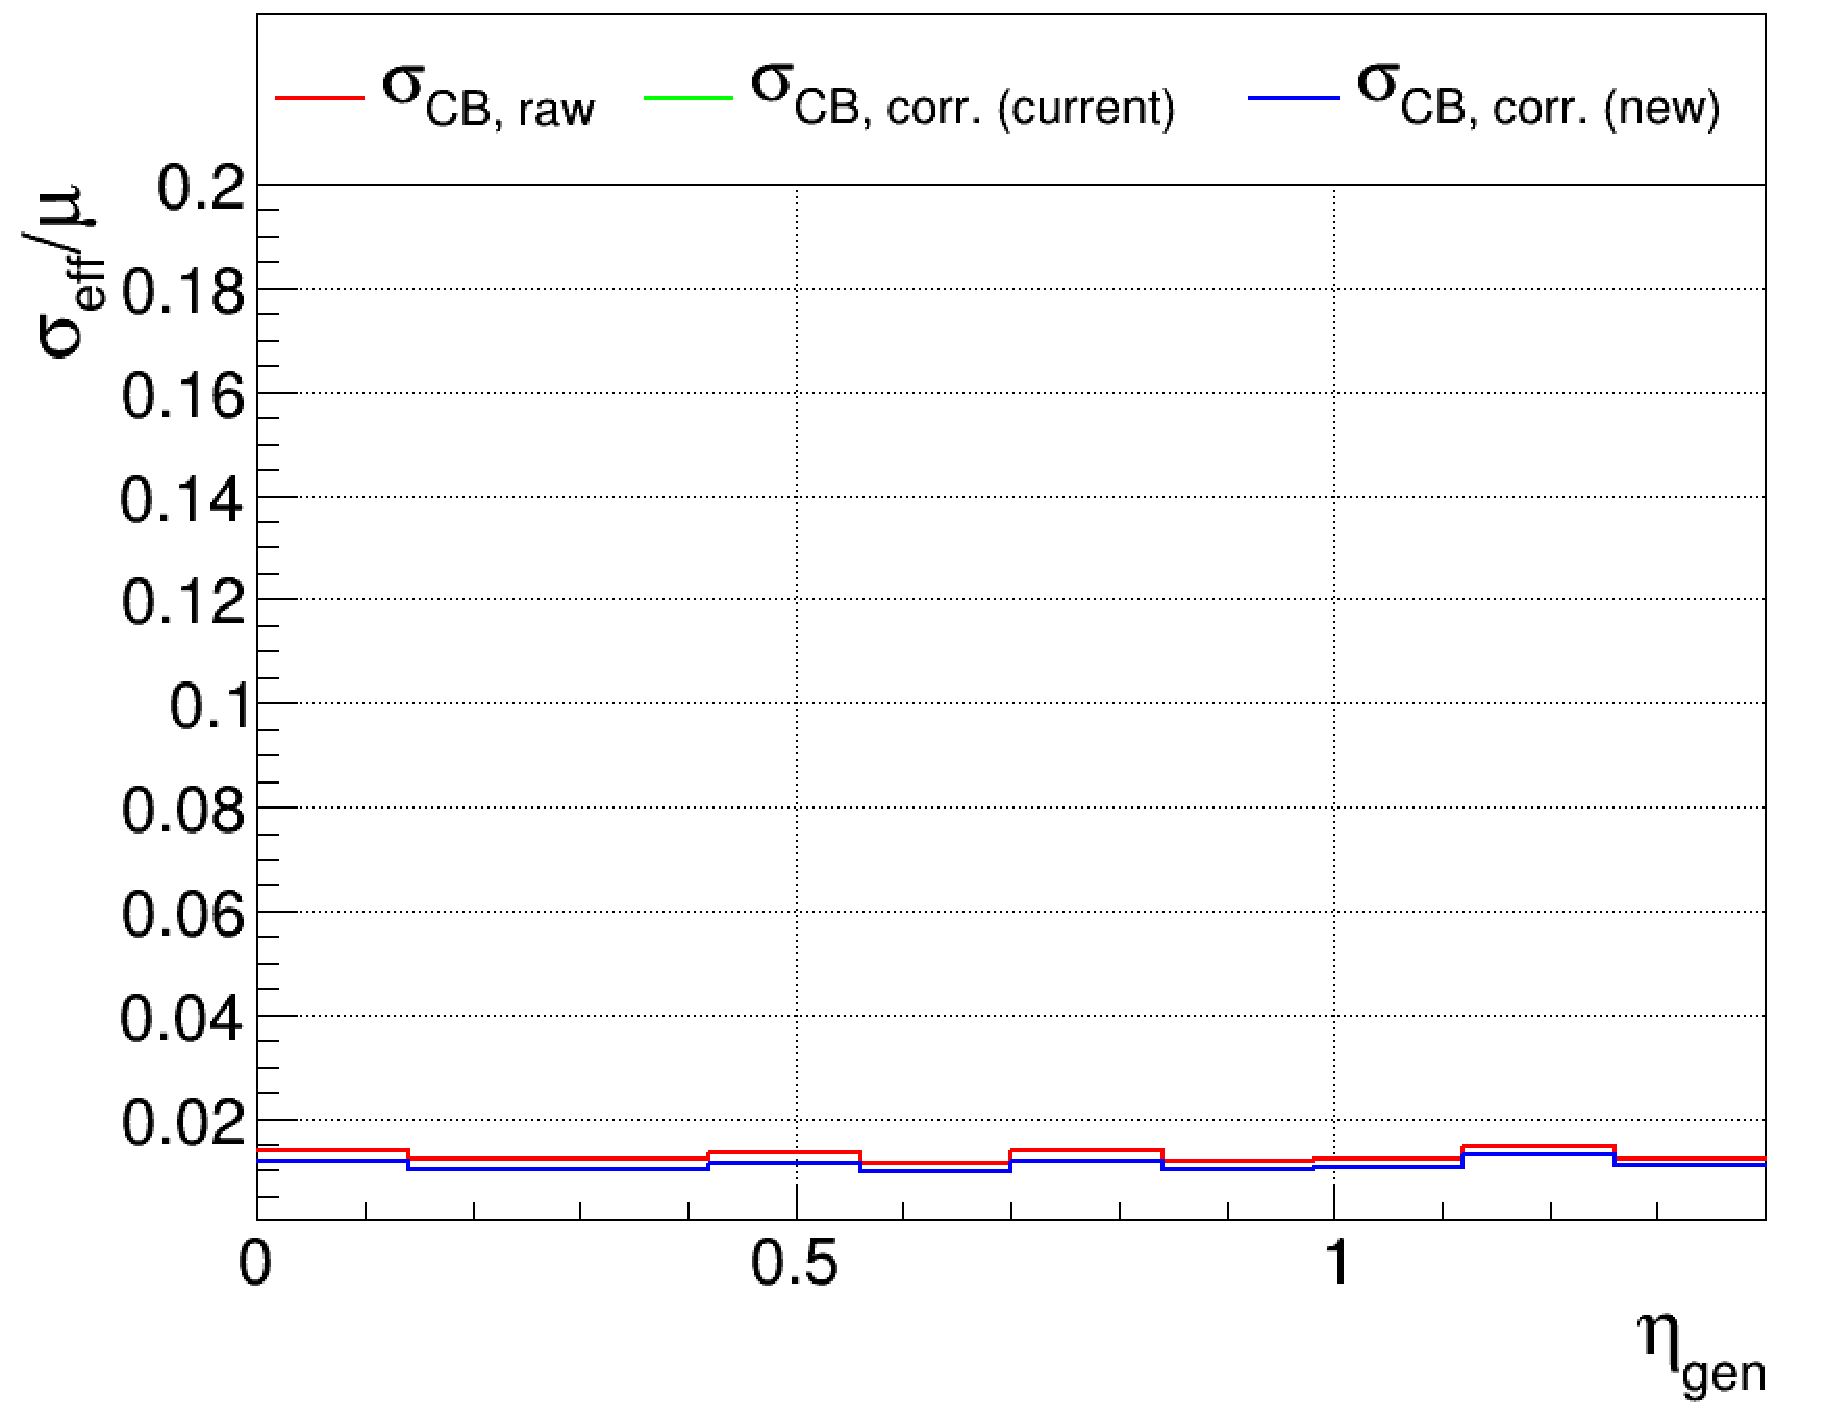
\includegraphics[width=0.495\textwidth]{./plots_pdf/ECAL_plots/plotsPU/EB/FULL/pdf/GENETA/EBFULL_GENETA_0100_0300_EffSigmaOverBins.pdf}
\caption{EB - Full Readout \pt 100-300\GeV}
\end{figure}





\begin{figure}
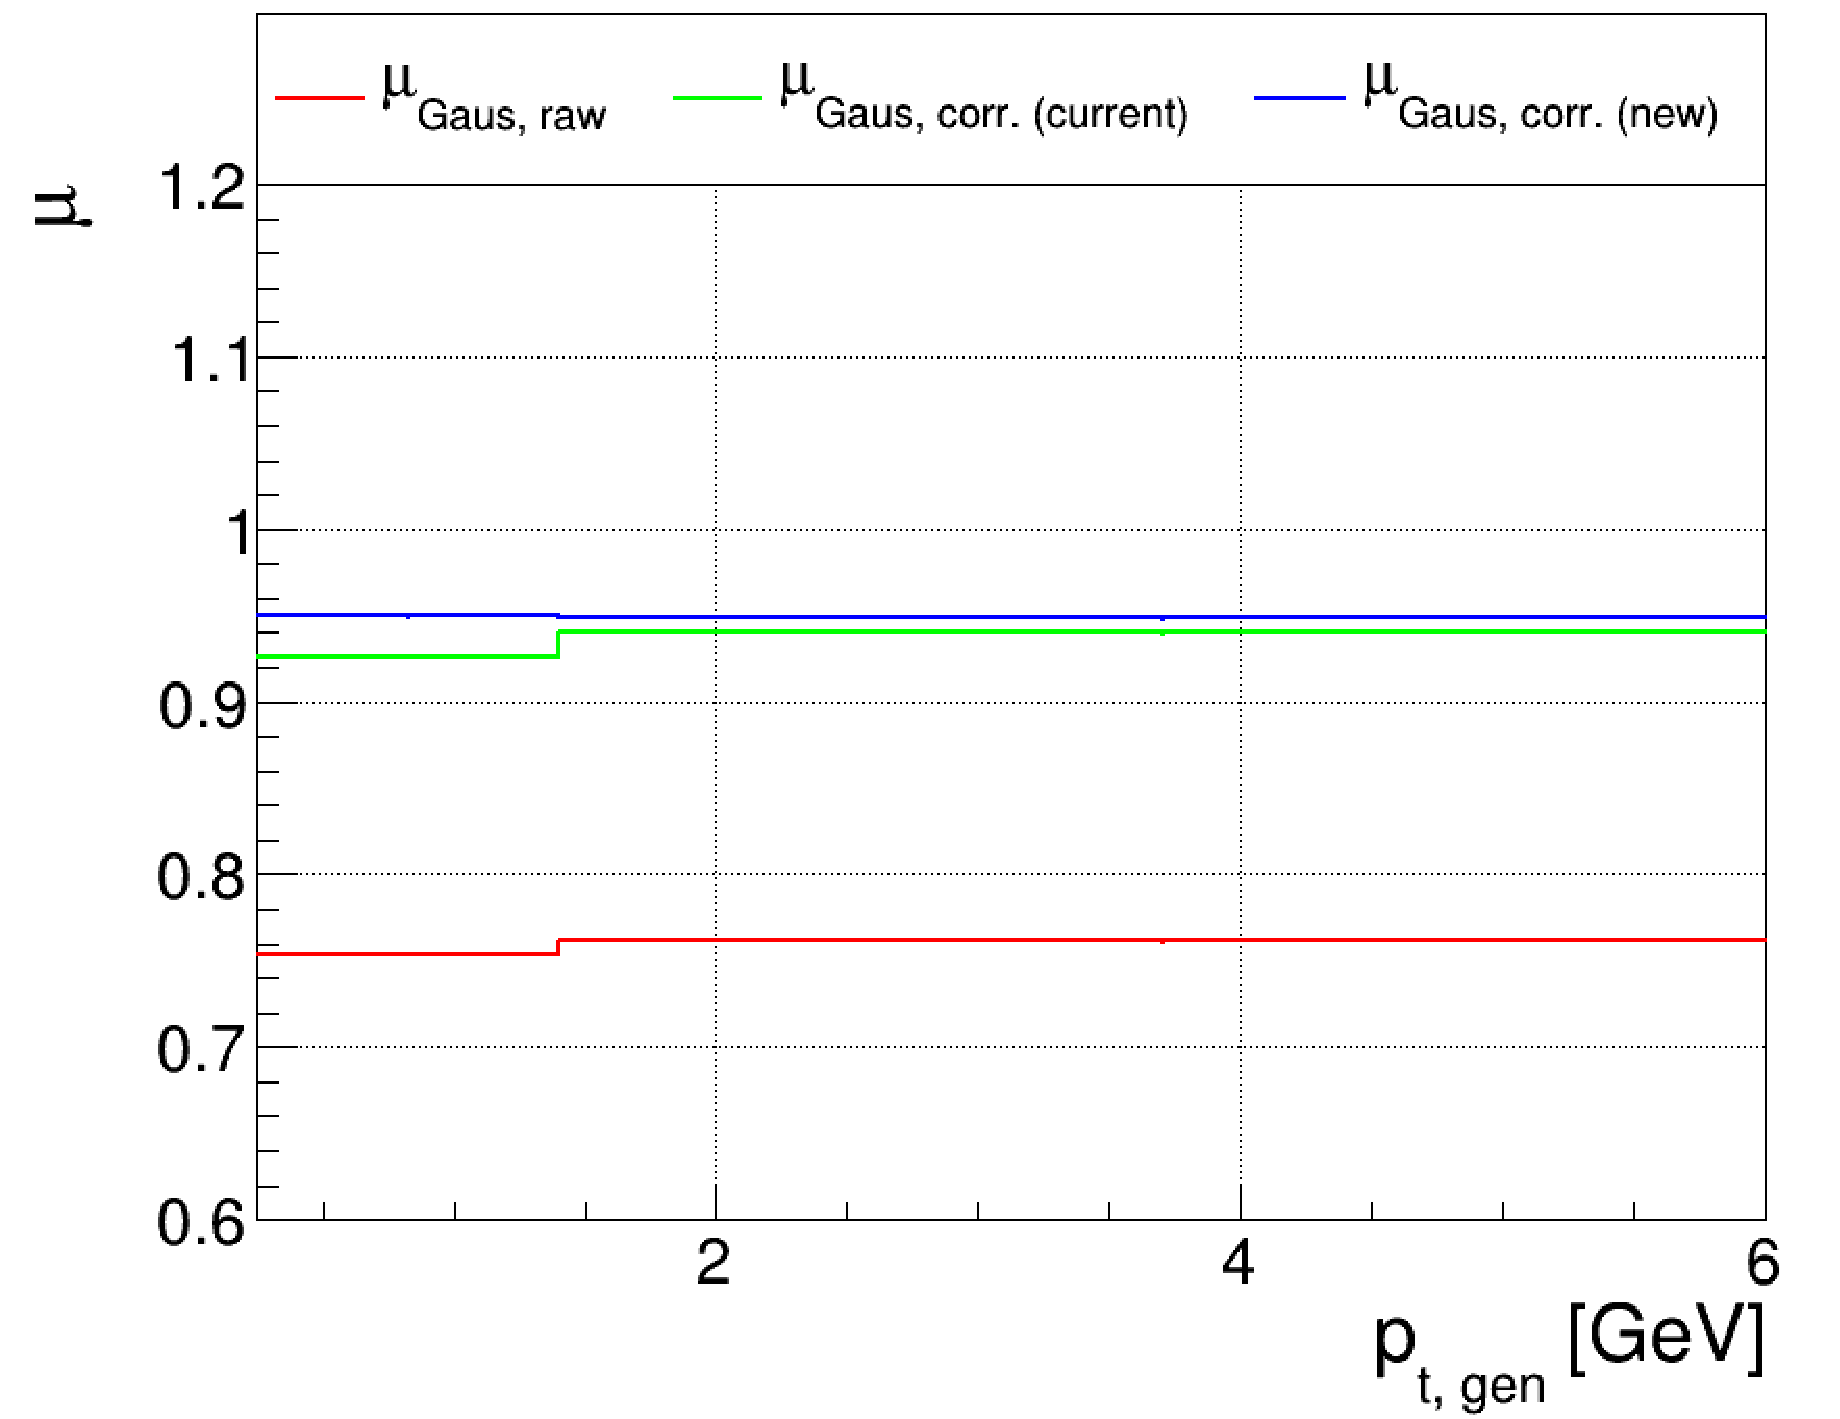
\includegraphics[width=0.495\textwidth]{./plots_pdf/ECAL_plots/plotsPU/EB/ZS/pdf/GENPT/EBZS_GENPT_0000_0006_MuOverBins.pdf}
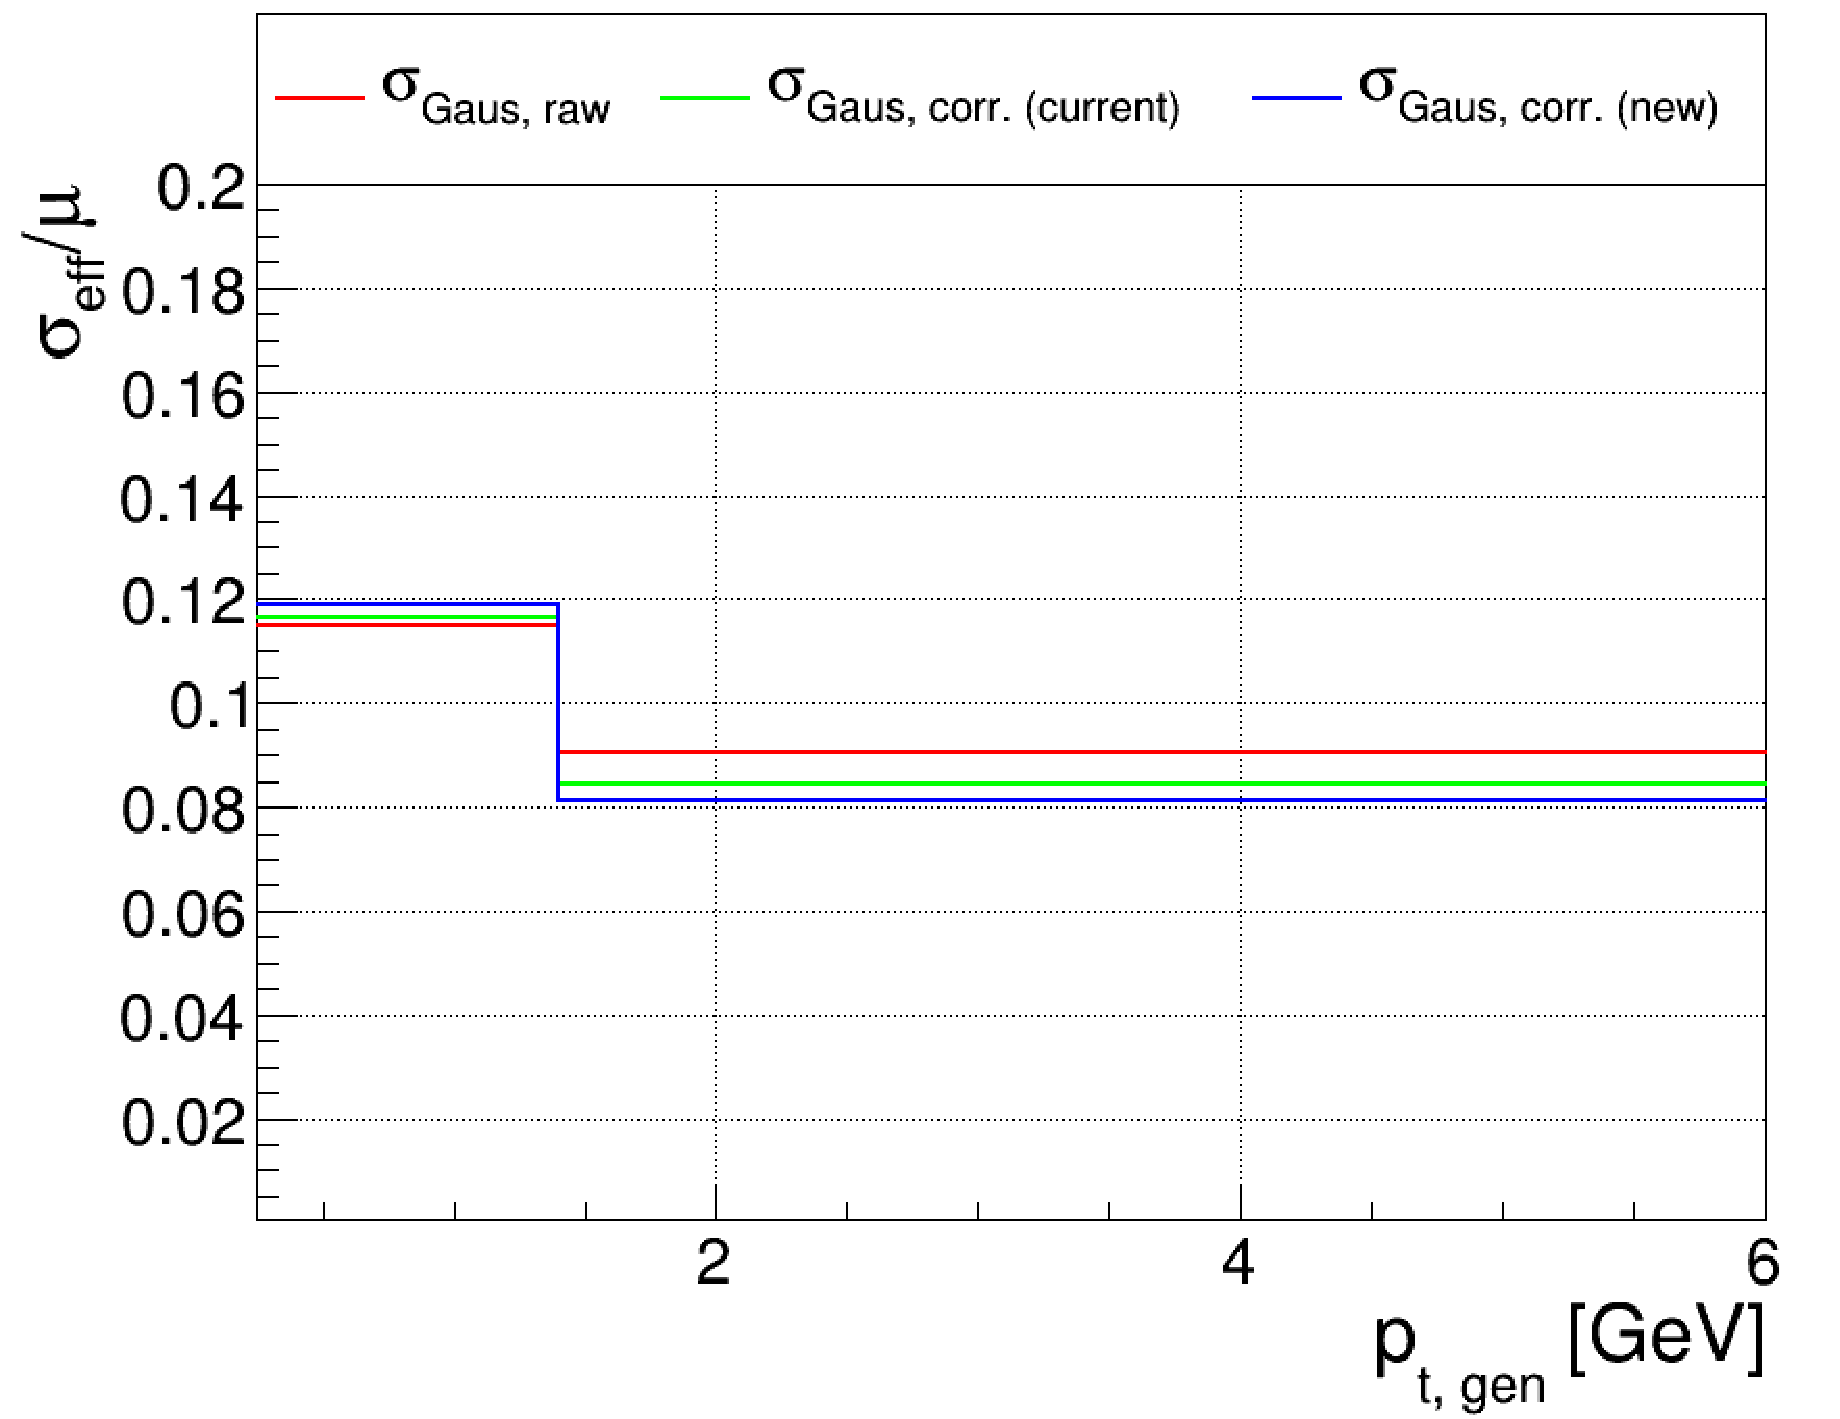
\includegraphics[width=0.495\textwidth]{./plots_pdf/ECAL_plots/plotsPU/EB/ZS/pdf/GENPT/EBZS_GENPT_0000_0006_EffSigmaOverBins.pdf}

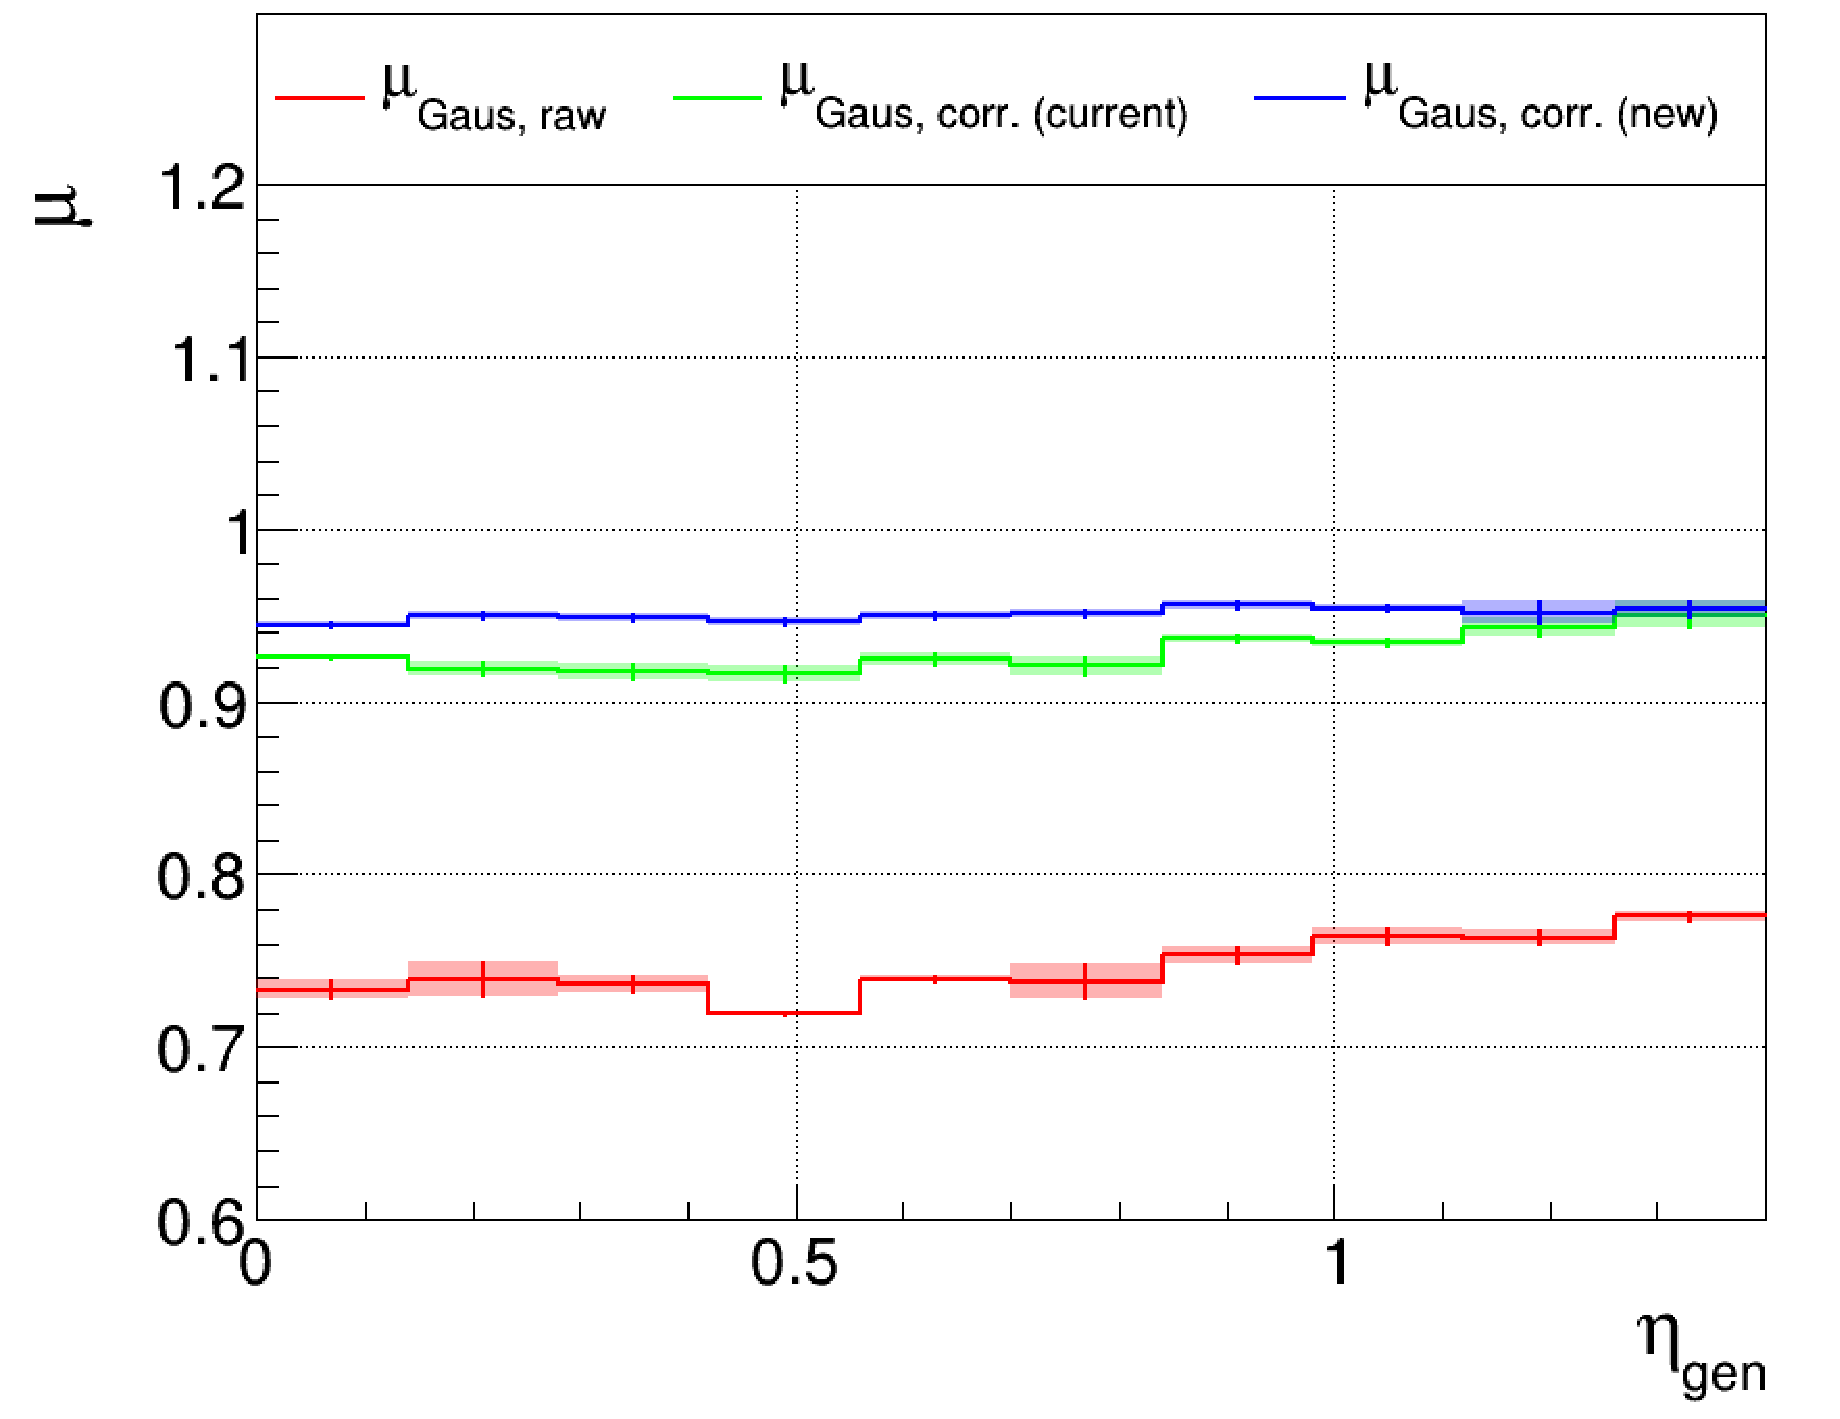
\includegraphics[width=0.495\textwidth]{./plots_pdf/ECAL_plots/plotsPU/EB/ZS/pdf/GENETA/EBZS_GENETA_0000_0006_MuOverBins.pdf}
\includegraphics[width=0.495\textwidth]{./plots_pdf/ECAL_plots/plotsPU/EB/ZS/pdf/GENETA/EBZS_GENETA_0000_0006_EffSigmaOverBins.pdf}
\caption[$\mu$ ($\sigma_\mathrm{eff}$) vs \pt of PF ECAL cluster - EB ZS readout PU  senario]{Mean response (resolution) defined by Raw PF ECAL clusters (red), the calibration derived earlier in Ru\
n3 based on 126X (green), and the new correction from 2024 simulation sample based on 133X (blue). \pt 0--6\GeV PU EB ZS readout PU senario.}
\label{fig:PU_EBZS}
\end{figure}

%% %\begin{figure}
%% \includegraphics[width=0.495\textwidth]{./plots_pdf/ECAL_plots/plotsPU/EB/ZS/pdf/GENPT/EBZS_GENPT_0006_0025_MuOverBins.pdf}
%% 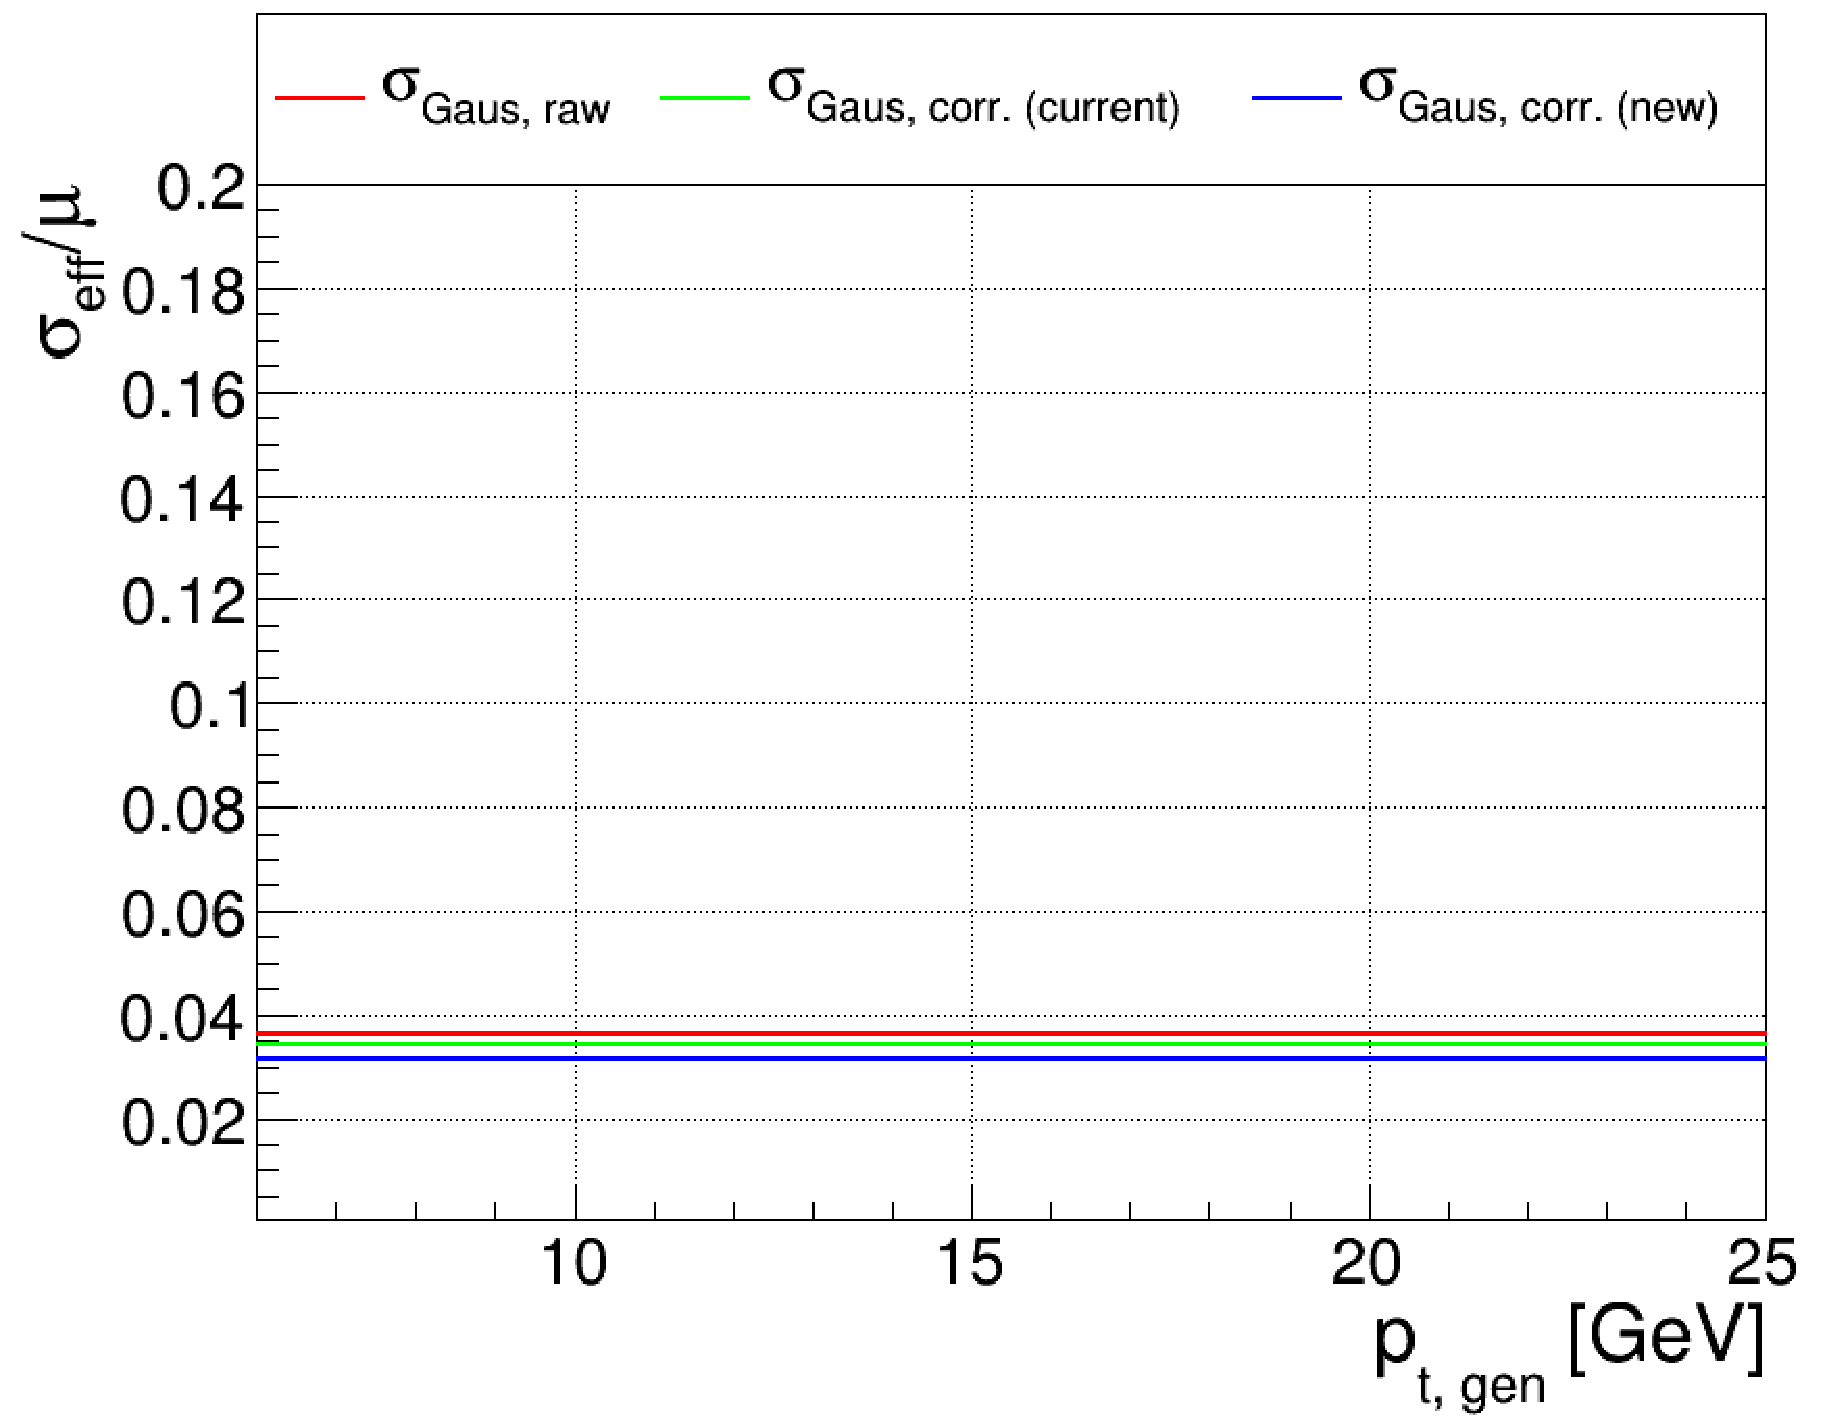
\includegraphics[width=0.495\textwidth]{./plots_pdf/ECAL_plots/plotsPU/EB/ZS/pdf/GENPT/EBZS_GENPT_0006_0025_EffSigmaOverBins.pdf}
%% %\caption{EB - ZS Readout pt 6-25}
%% %\end{figure}
%% %\begin{figure}
%% 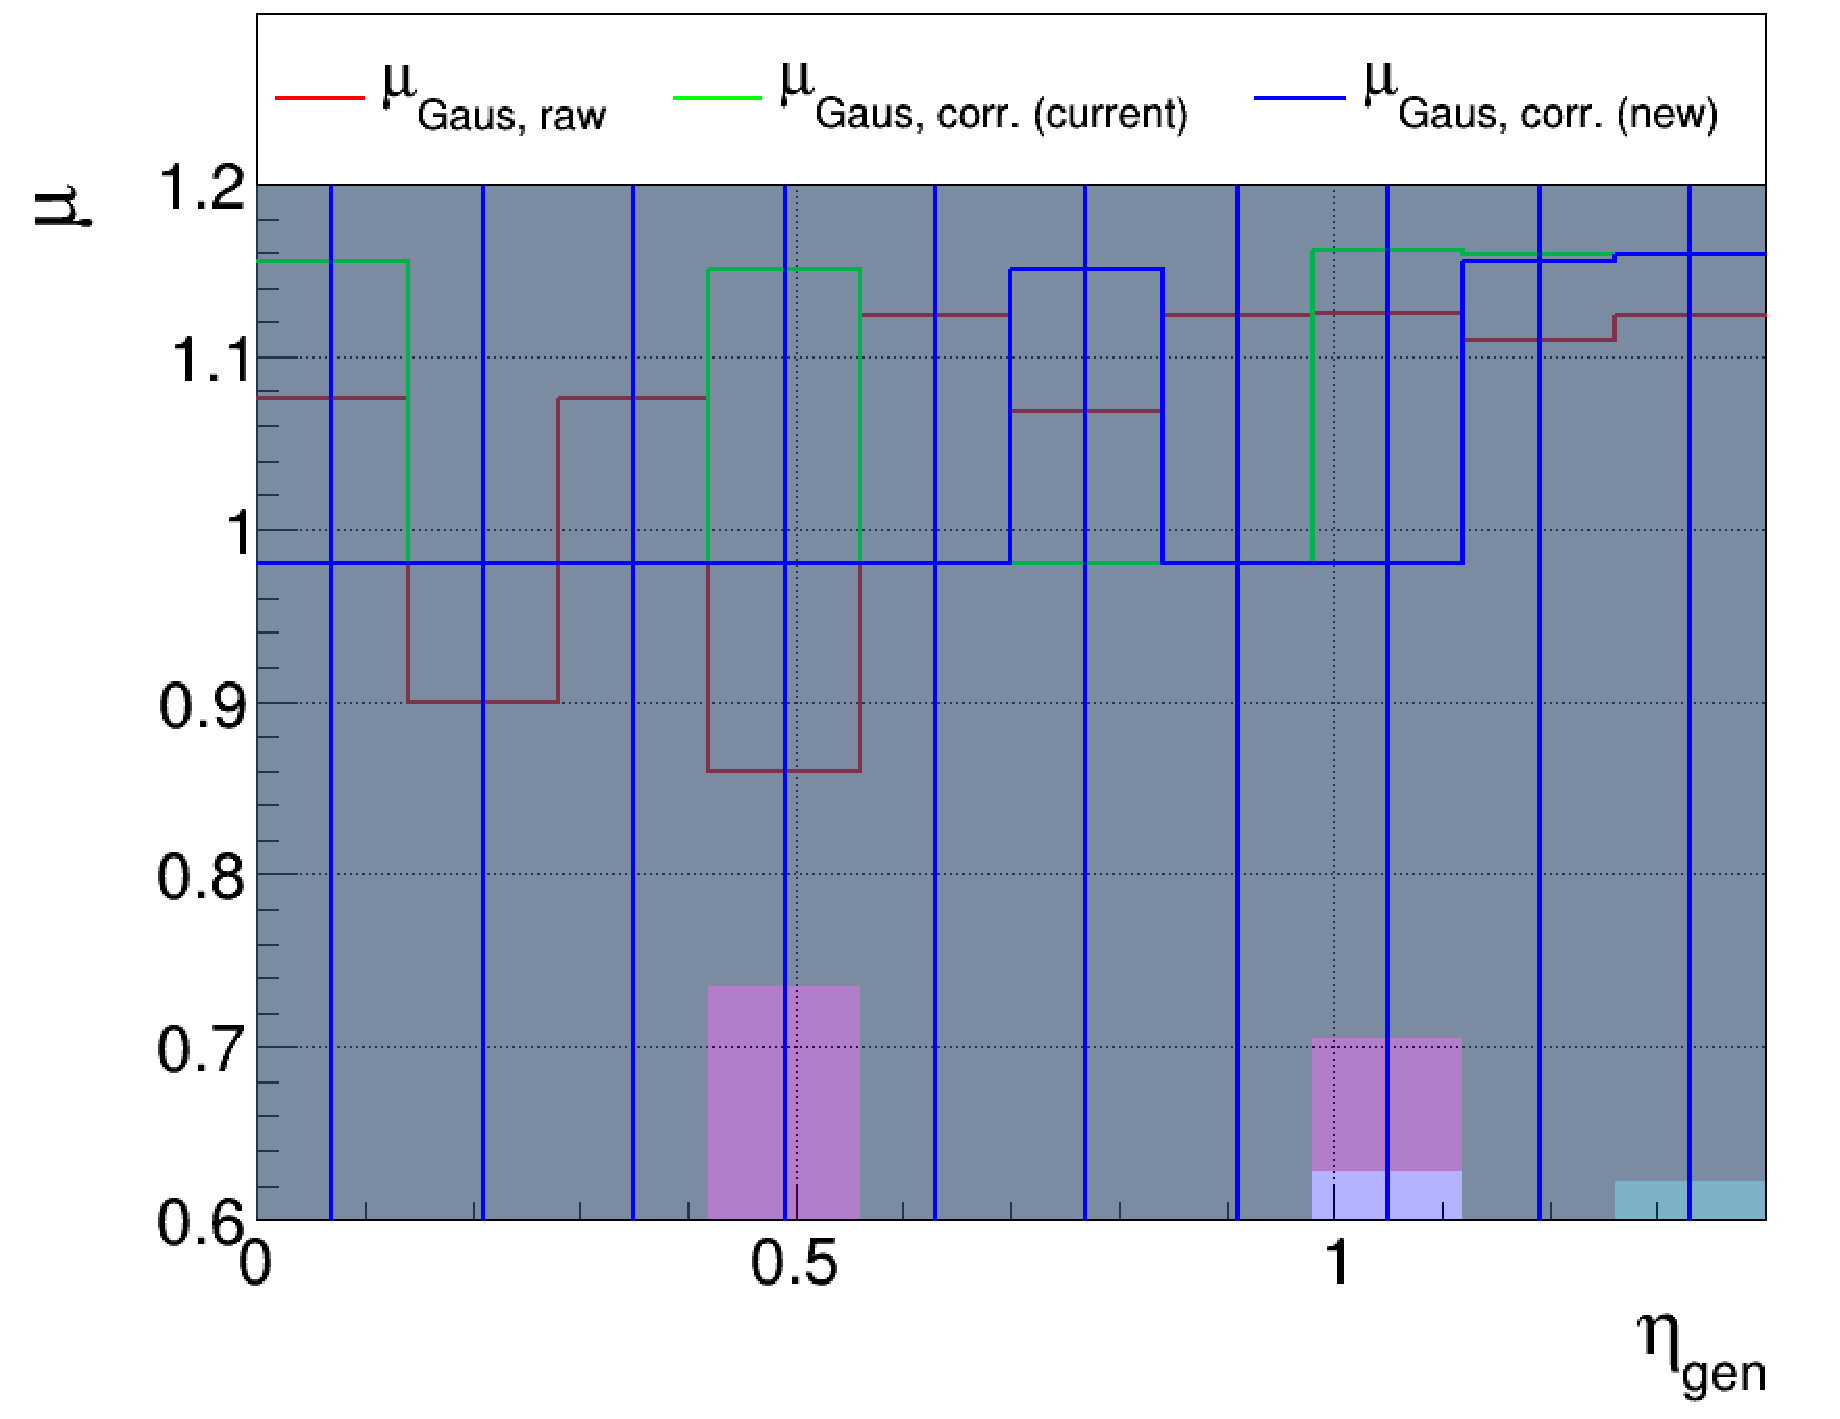
\includegraphics[width=0.495\textwidth]{./plots_pdf/ECAL_plots/plotsPU/EB/ZS/pdf/GENETA/EBZS_GENETA_0006_0025_MuOverBins.pdf}
%% 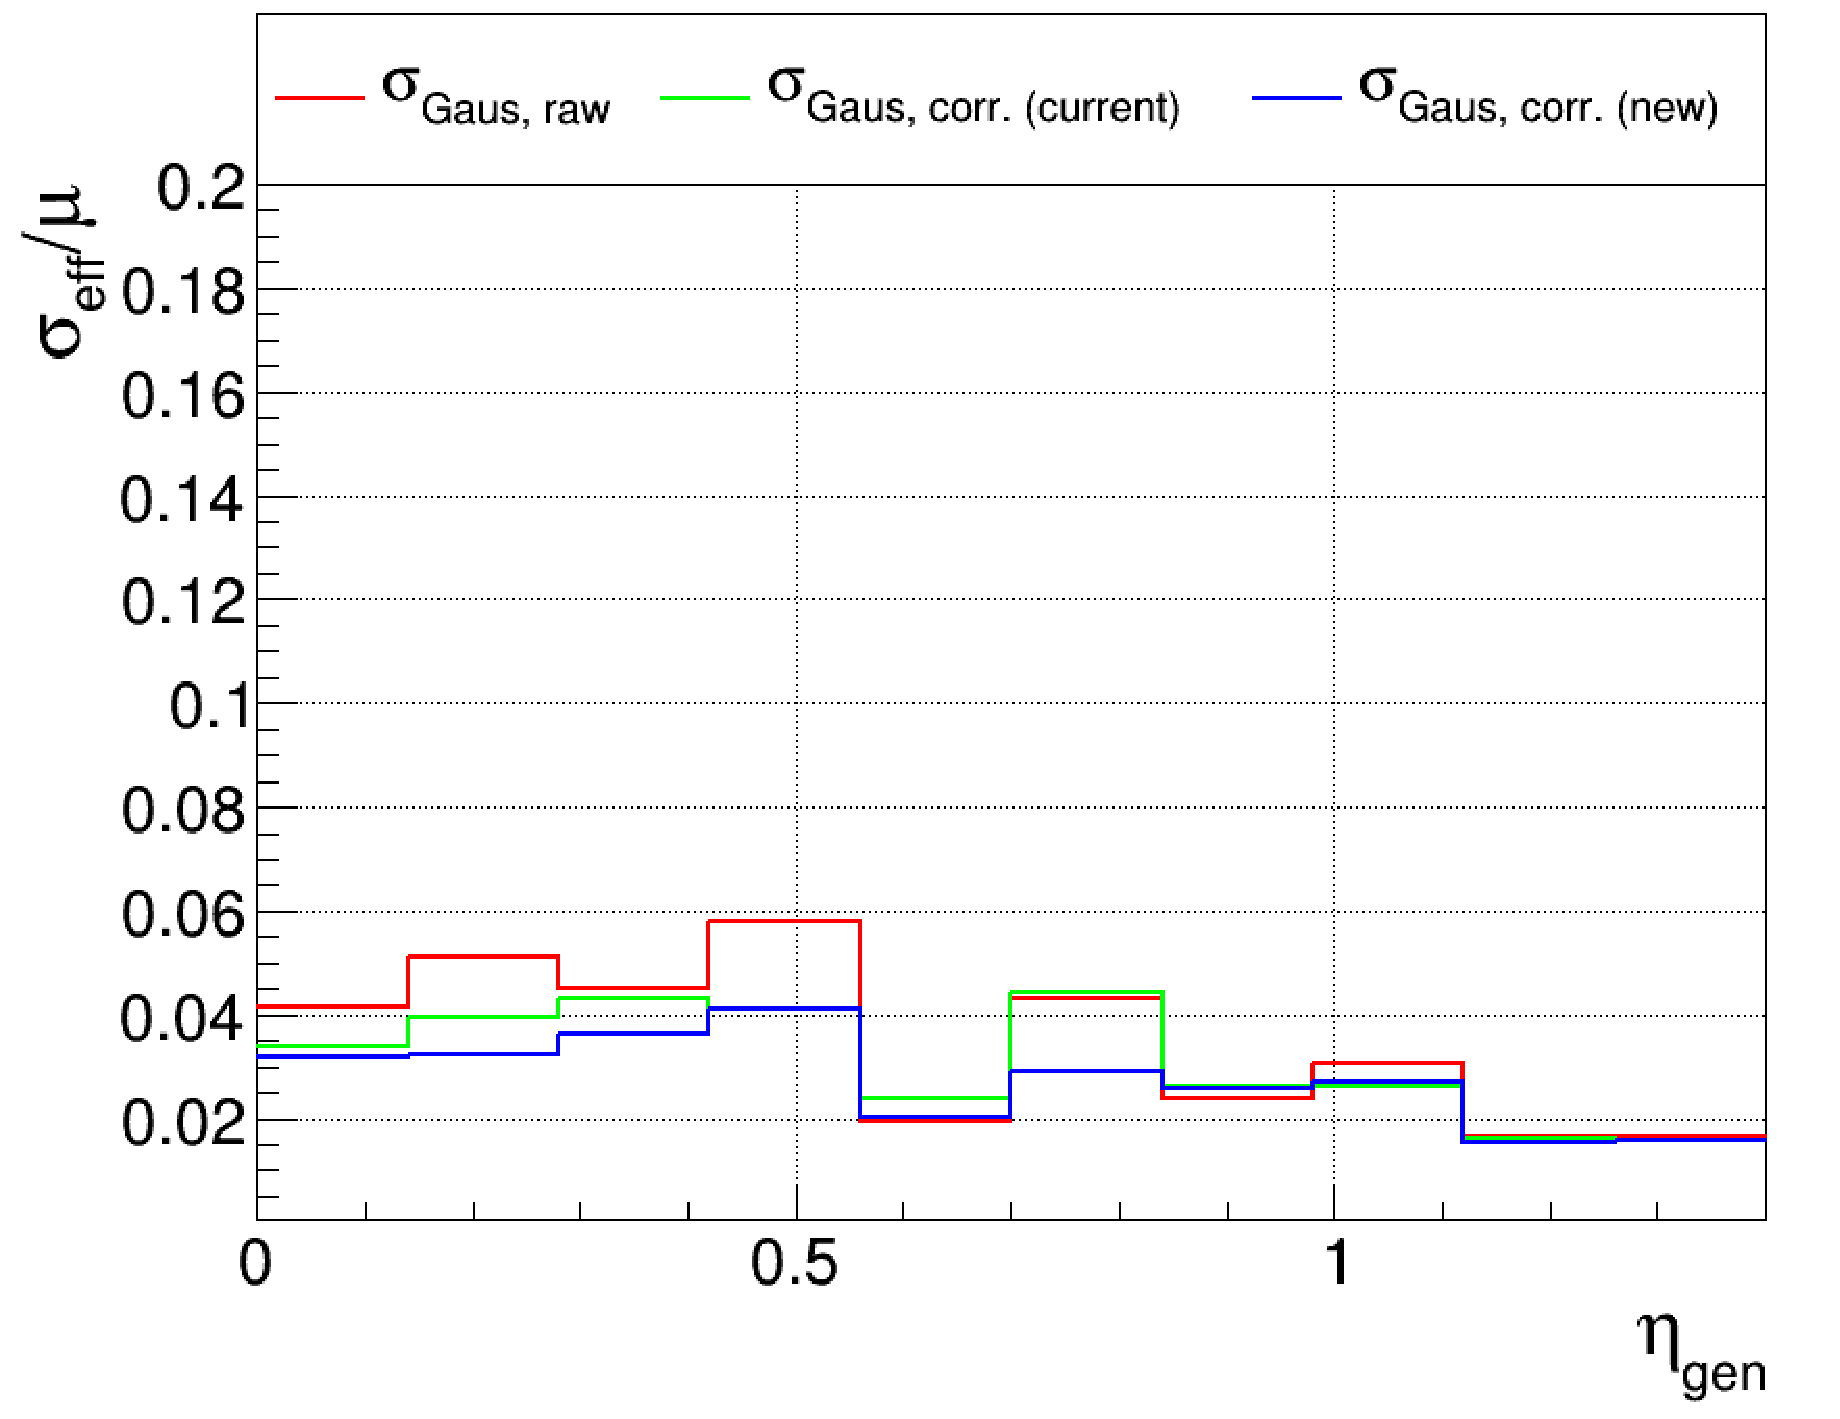
\includegraphics[width=0.495\textwidth]{./plots_pdf/ECAL_plots/plotsPU/EB/ZS/pdf/GENETA/EBZS_GENETA_0006_0025_EffSigmaOverBins.pdf}
%% \caption{EB - ZS Readout \pt 6-25}
%% \end{figure}







\begin{figure}
  %5-20 pt 
\includegraphics[width=0.335\textwidth]{./plots_pdf/ECAL_plots/plotsNOPU/EB/FULL/pdf/GENPT/EBFULL_GENPT_0005_0020_MuOverBins.pdf}
\includegraphics[width=0.3355\textwidth]{./plots_pdf/ECAL_plots/plotsNOPU/EB/FULL/pdf/GENPT/EBFULL_GENPT_0005_0020_EffSigmaOverBins.pdf}

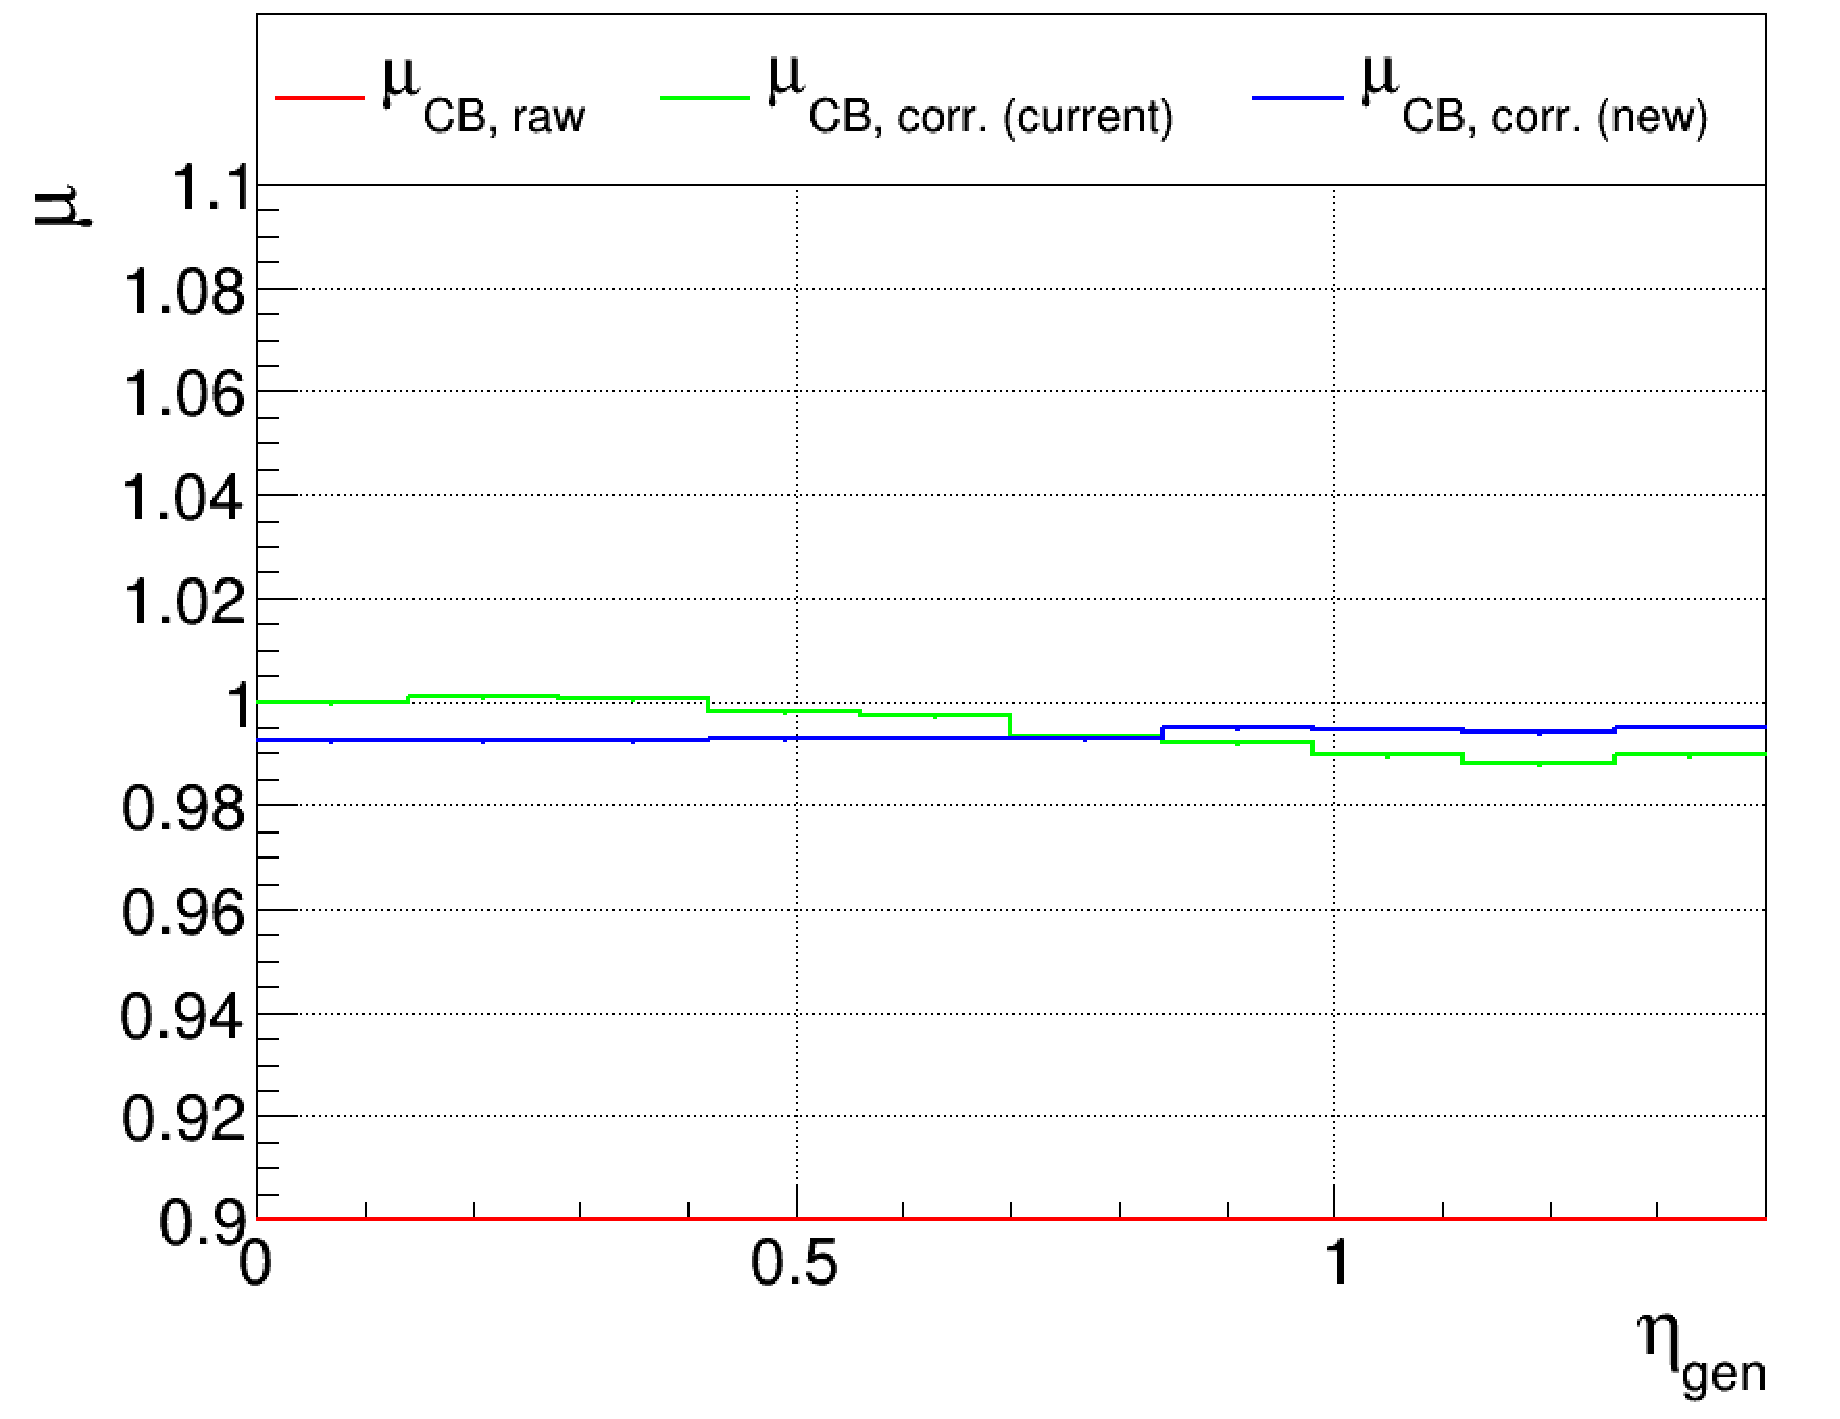
\includegraphics[width=0.495\textwidth]{./plots_pdf/ECAL_plots/plotsNOPU/EB/FULL/pdf/GENETA/EBFULL_GENETA_0005_0020_MuOverBins.pdf}
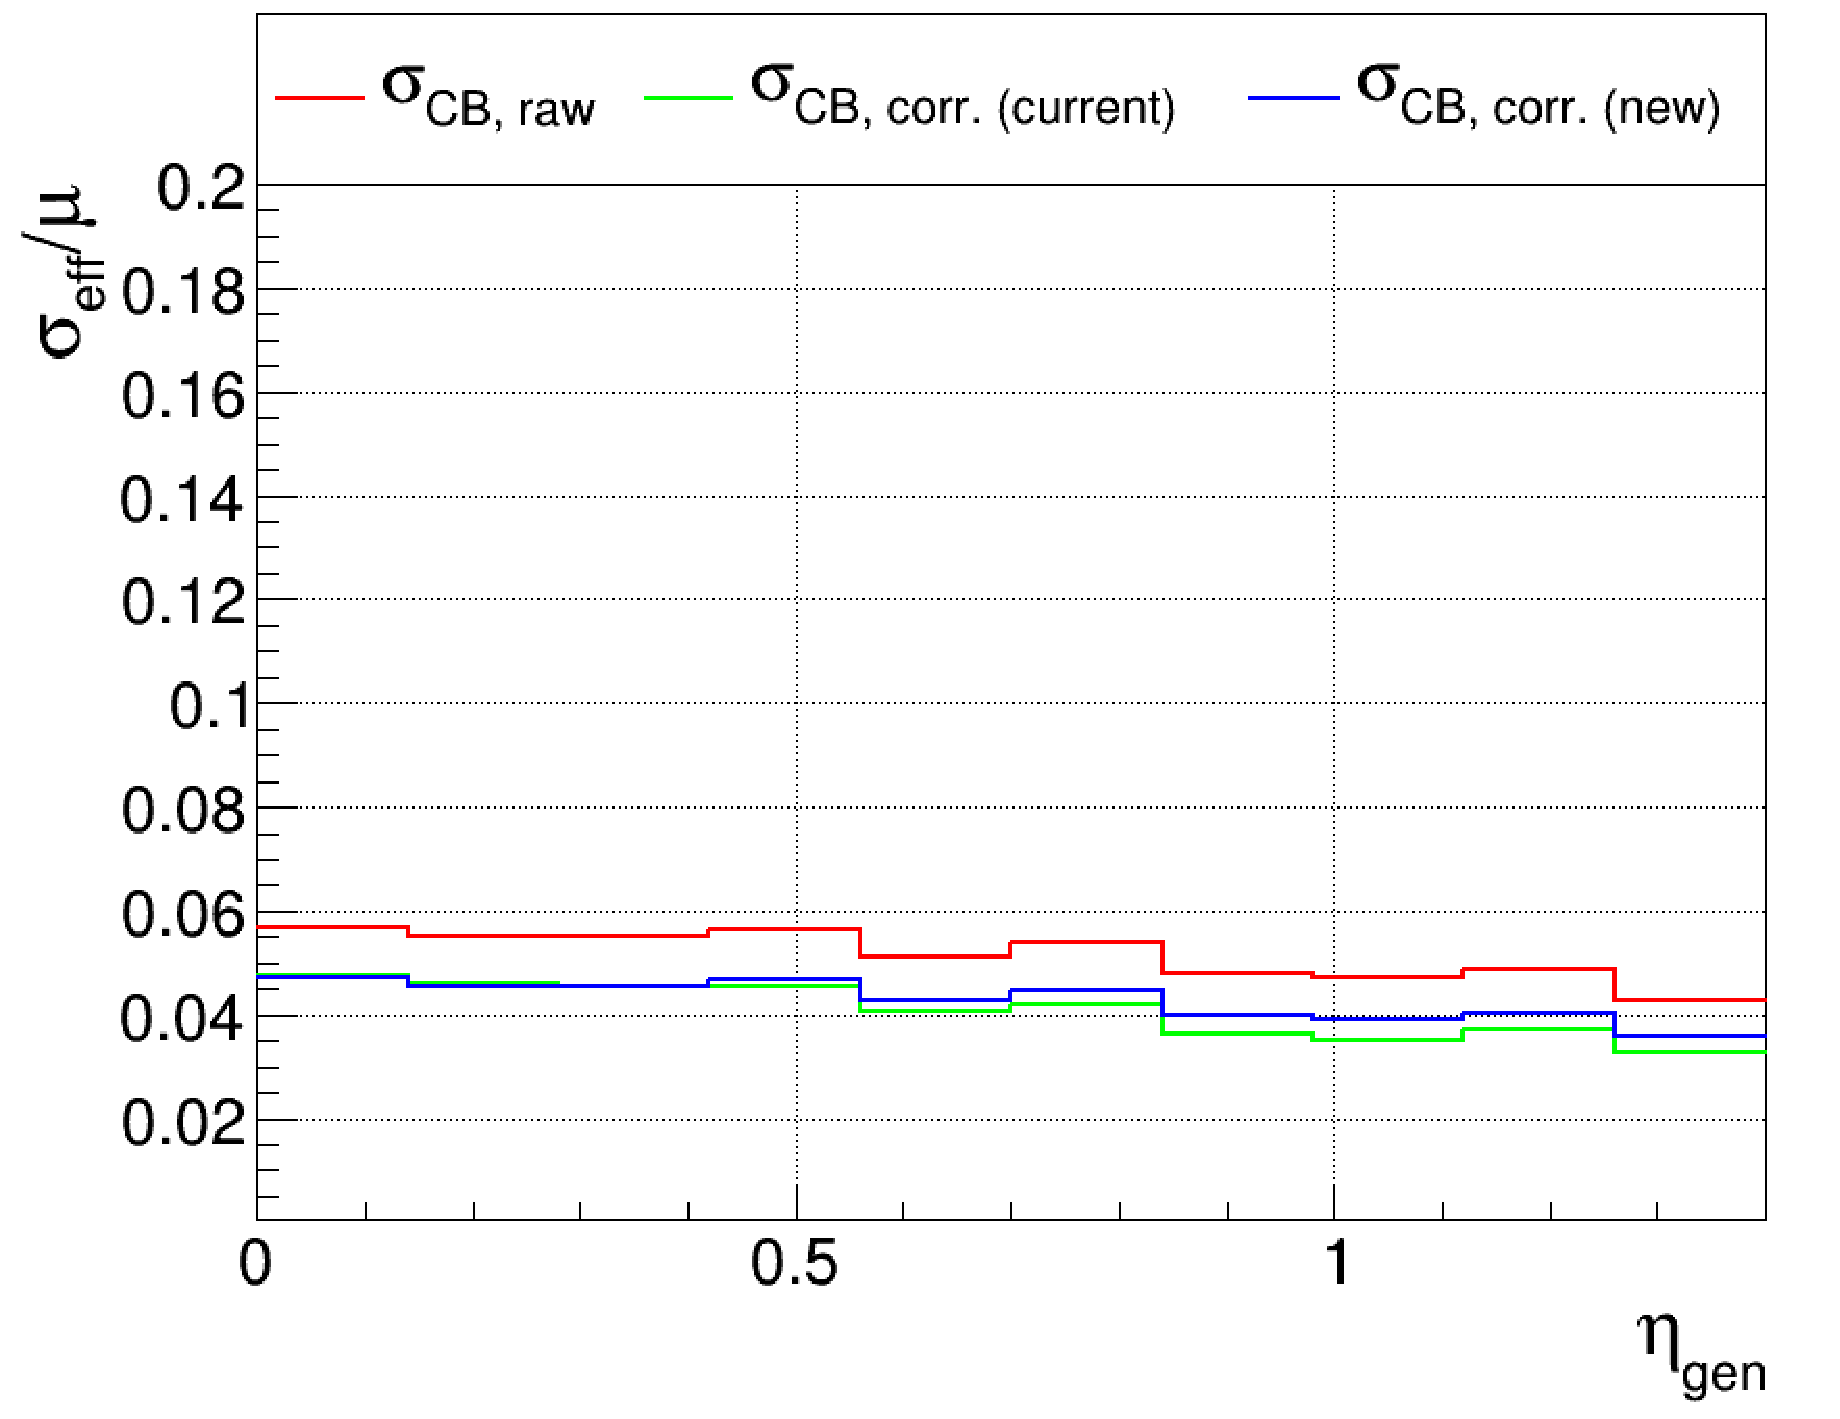
\includegraphics[width=0.495\textwidth]{./plots_pdf/ECAL_plots/plotsPU/EB/FULL/pdf/GENETA/EBFULL_GENETA_0005_0020_EffSigmaOverBins.pdf}
\caption{EB - Full Readout \pt 5-20}

%\begin{figure}
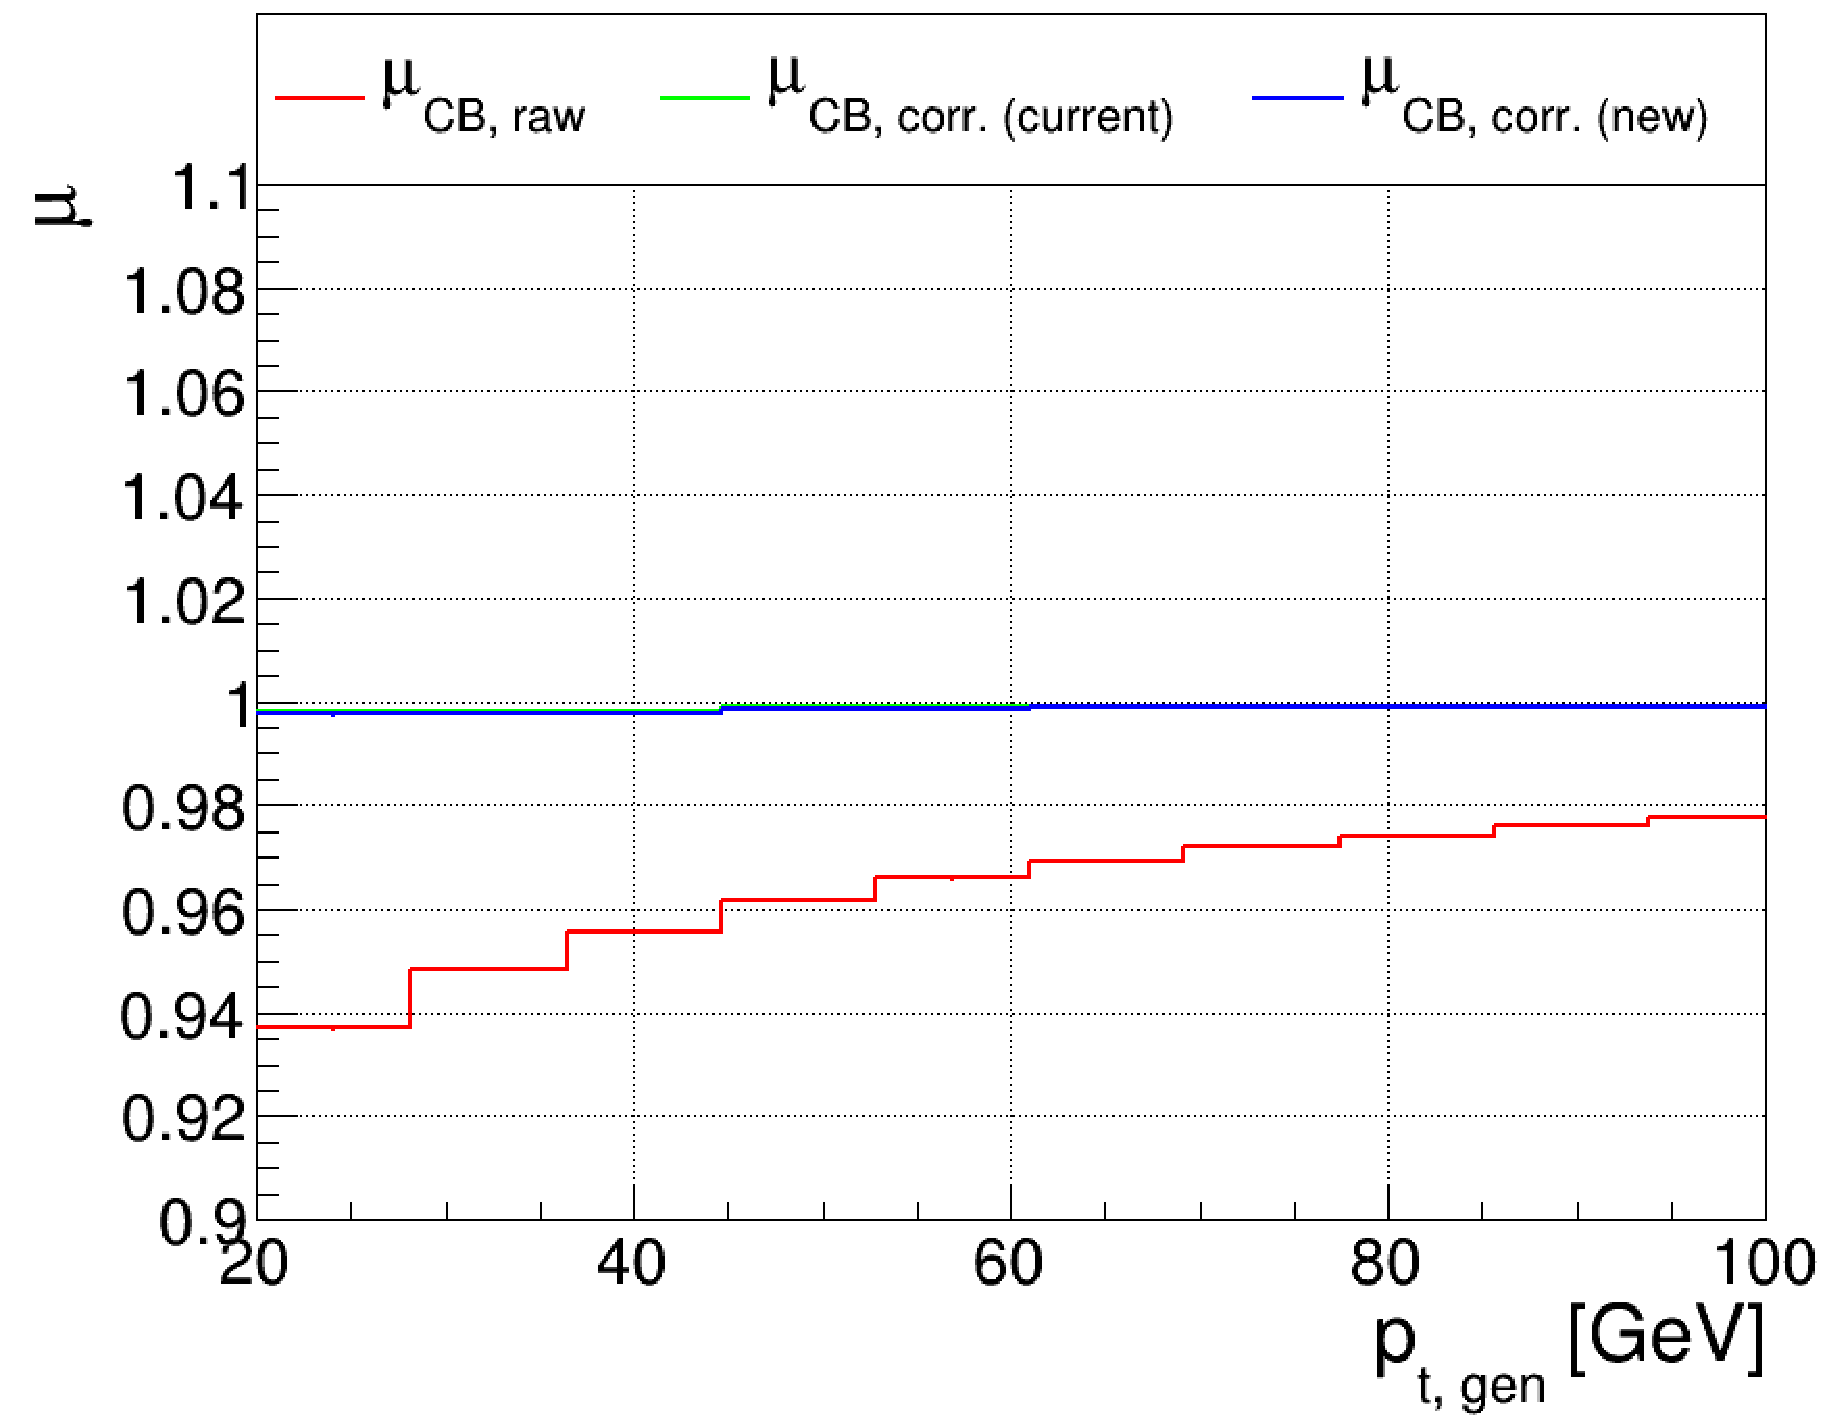
\includegraphics[width=0.495\textwidth]{./plots_pdf/ECAL_plots/plotsNOPU/EB/FULL/pdf/GENPT/EBFULL_GENPT_0020_0100_MuOverBins.pdf}
\includegraphics[width=0.495\textwidth]{./plots_pdf/ECAL_plots/plotsNOPU/EB/FULL/pdf/GENPT/EBFULL_GENPT_0020_0100_EffSigmaOverBins.pdf}

\includegraphics[width=0.495\textwidth]{./plots_pdf/ECAL_plots/plotsNOPU/EB/FULL/pdf/GENETA/EBFULL_GENETA_0020_0100_MuOverBins.pdf}
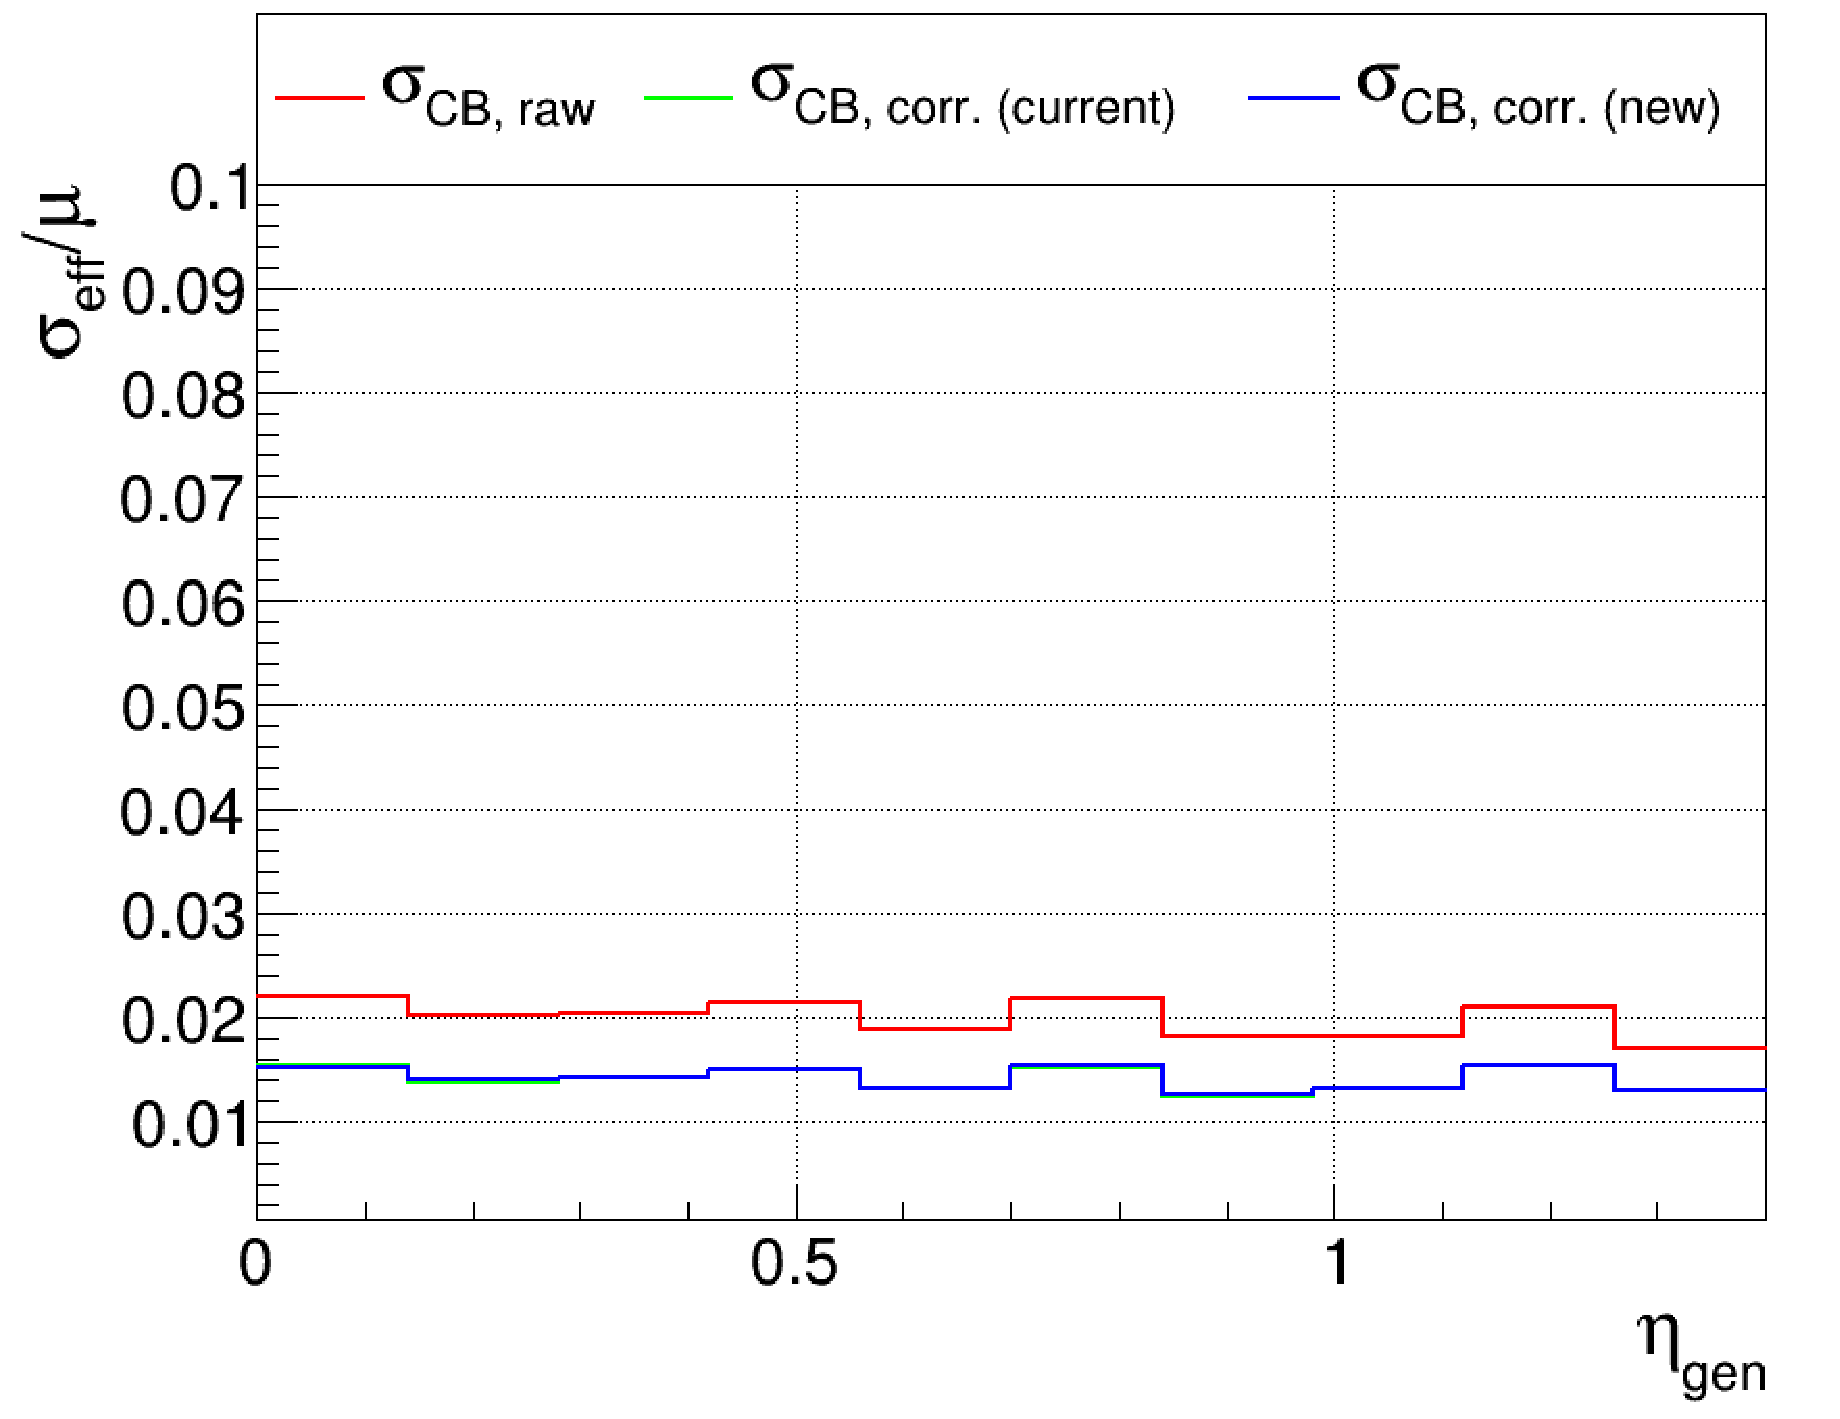
\includegraphics[width=0.495\textwidth]{./plots_pdf/ECAL_plots/plotsPU/EB/FULL/pdf/GENETA/EBFULL_GENETA_0020_0100_EffSigmaOverBins.pdf}
\caption{EB - Full Readout \pt 20-100}
\end{figure}


\begin{figure}
\includegraphics[width=0.495\textwidth]{./plots_pdf/ECAL_plots/plotsNOPU/EB/FULL/pdf/GENPT/EBFULL_GENPT_0100_0300_MuOverBins.pdf}
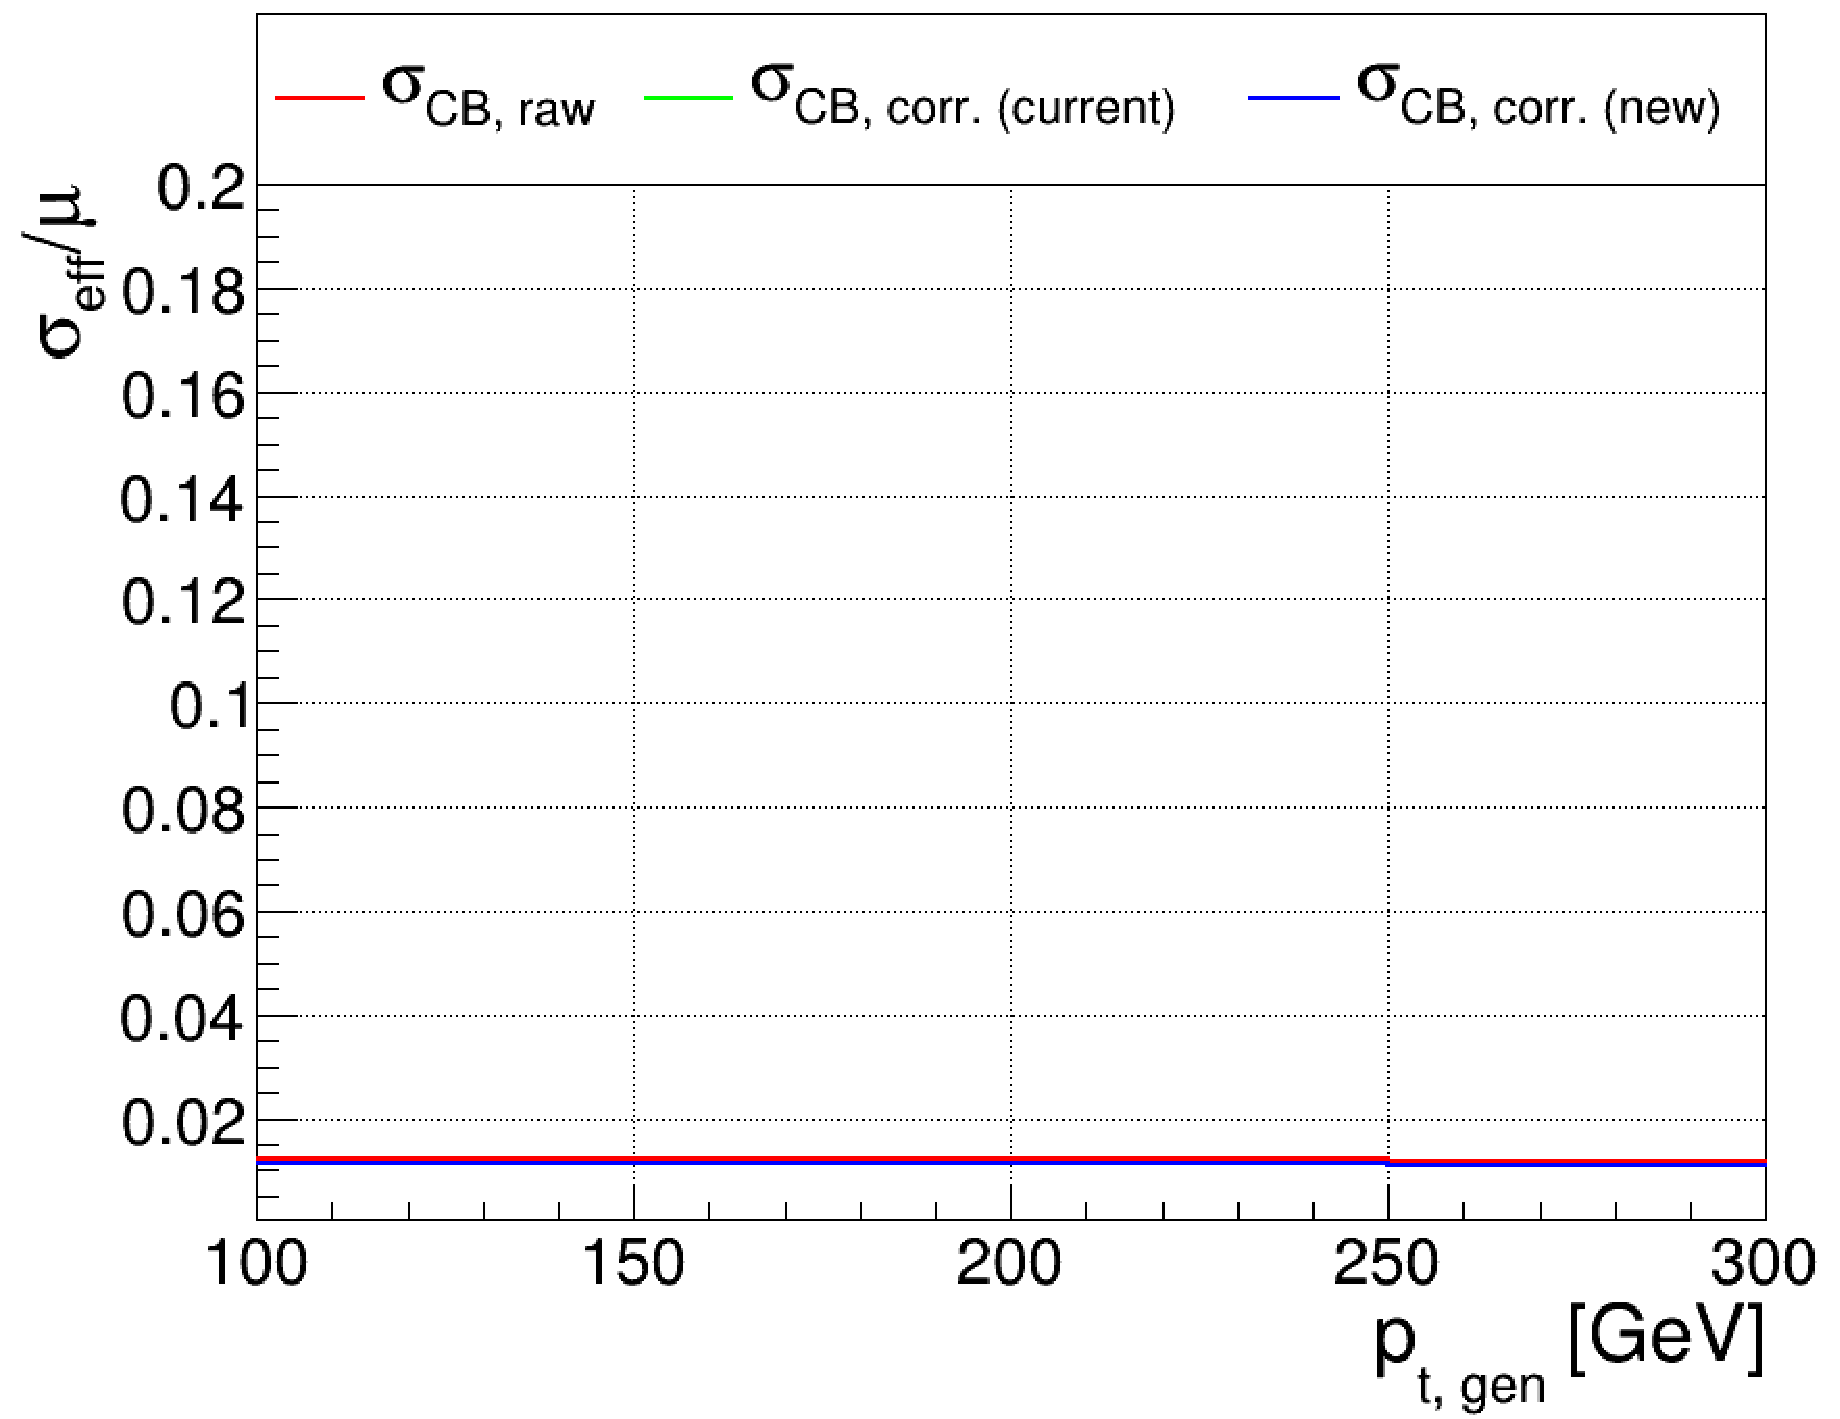
\includegraphics[width=0.495\textwidth]{./plots_pdf/ECAL_plots/plotsPU/EB/FULL/pdf/GENPT/EBFULL_GENPT_0100_0300_EffSigmaOverBins.pdf}


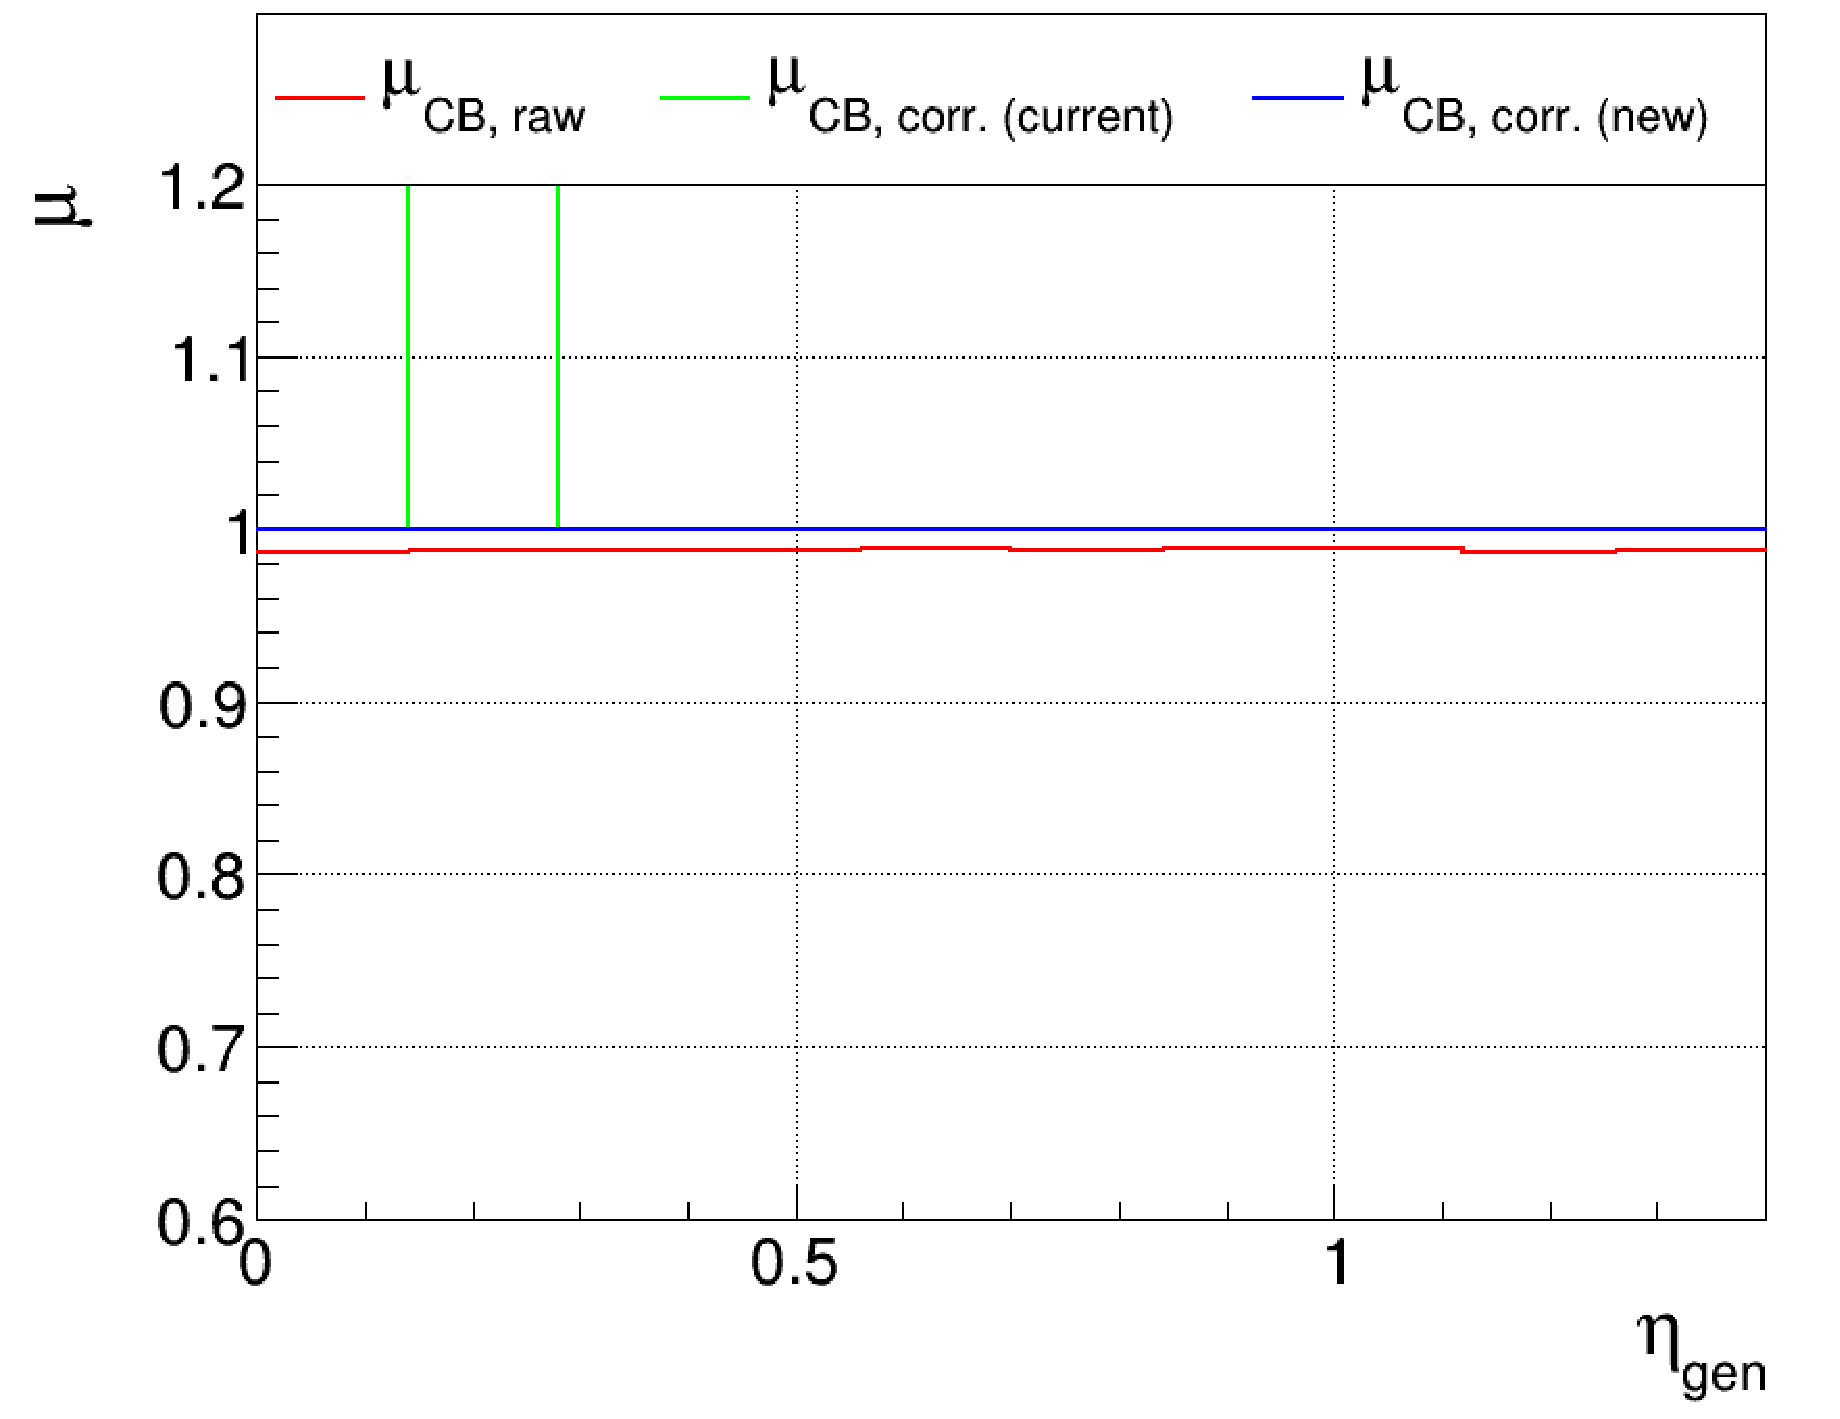
\includegraphics[width=0.495\textwidth]{./plots_pdf/ECAL_plots/plotsNOPU/EB/FULL/pdf/GENETA/EBFULL_GENETA_0100_0300_MuOverBins.pdf}
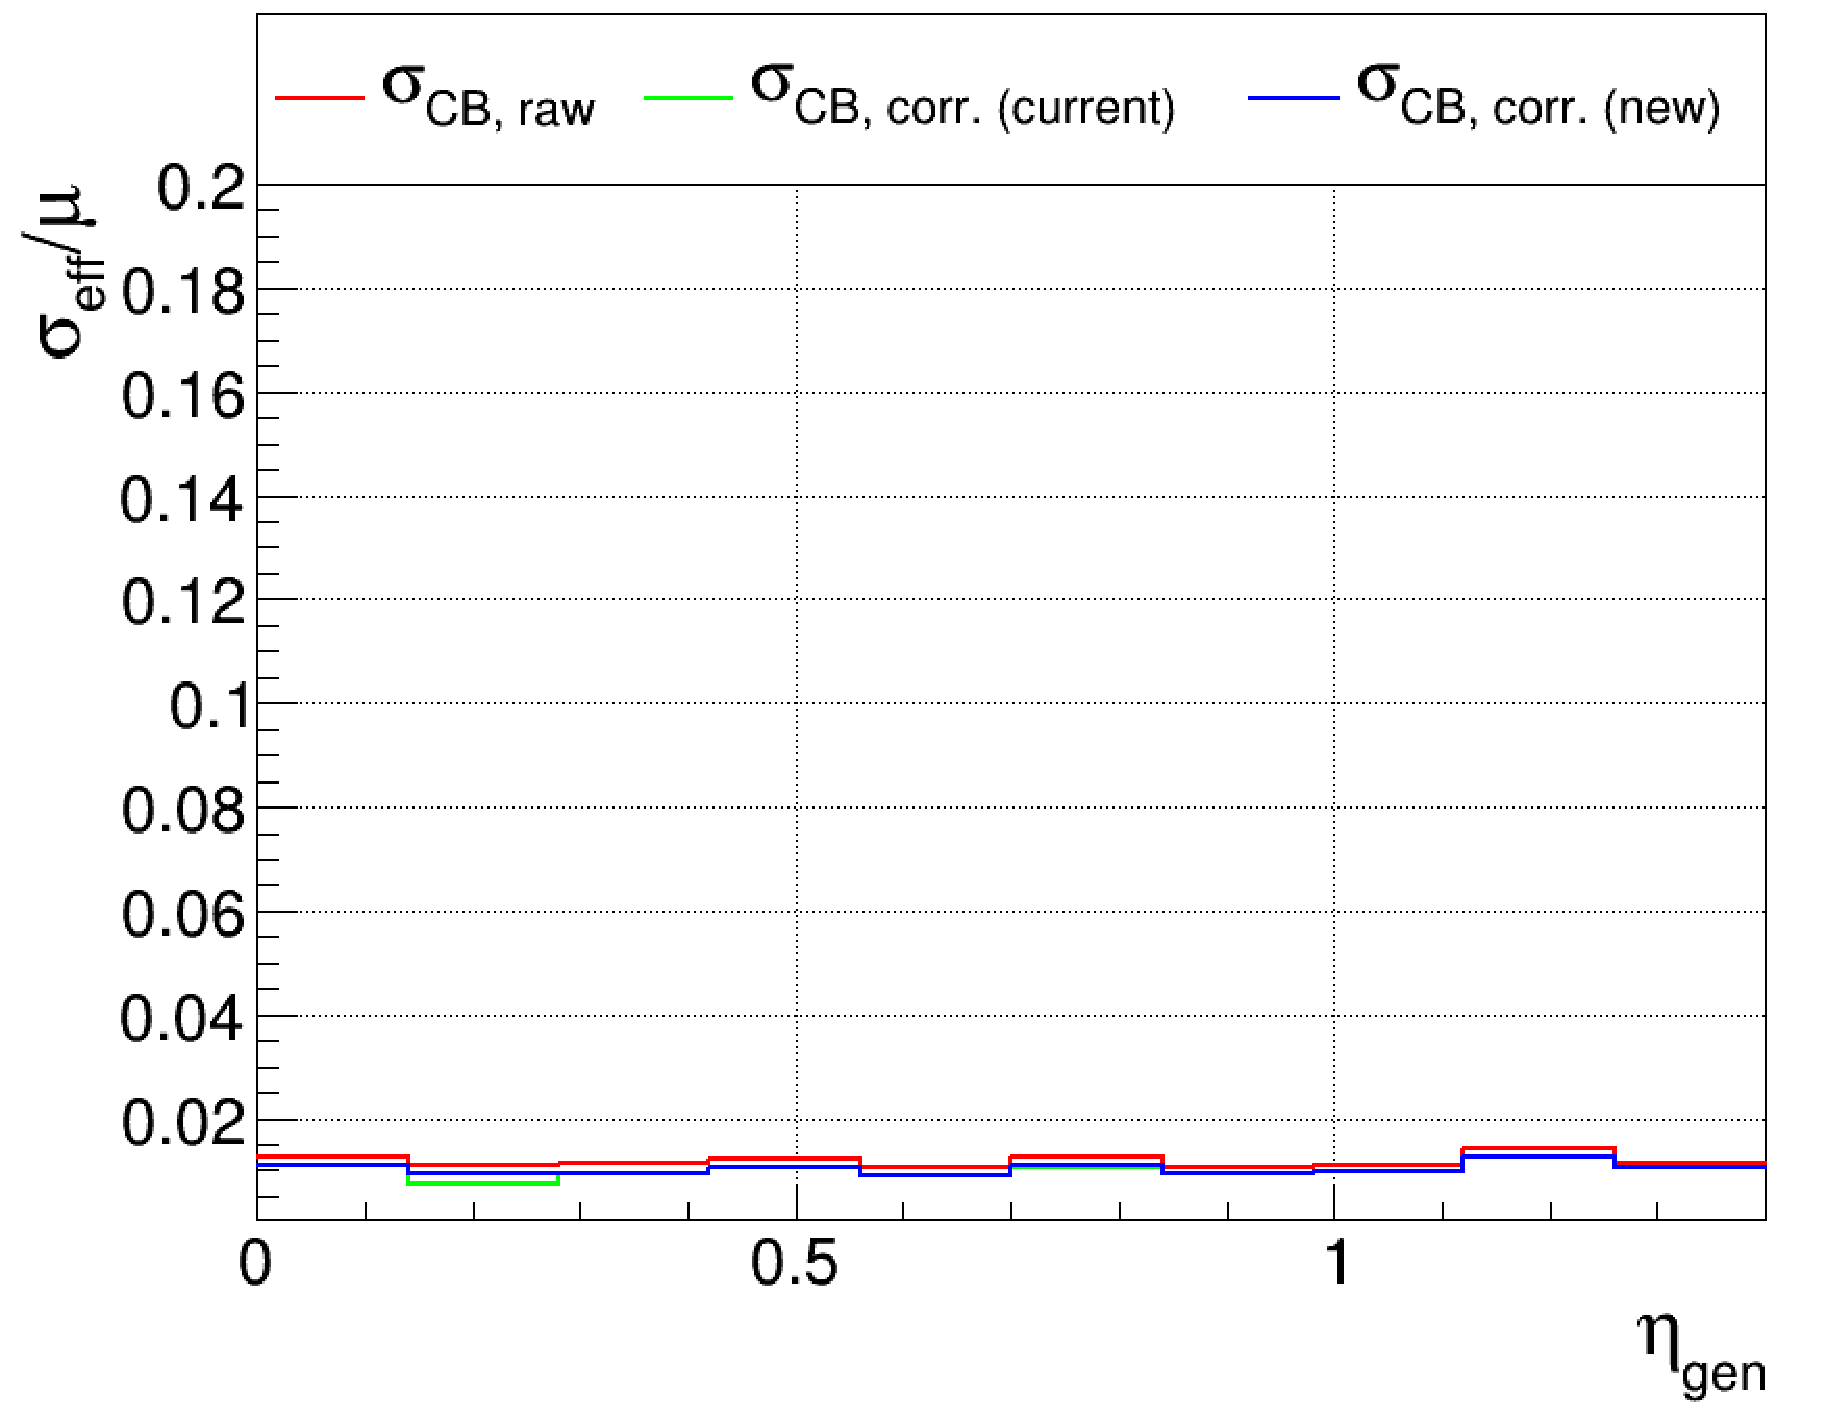
\includegraphics[width=0.495\textwidth]{./plots_pdf/ECAL_plots/plotsNOPU/EB/FULL/pdf/GENETA/EBFULL_GENETA_0100_0300_EffSigmaOverBins.pdf}
\caption{EB - Full Readout \pt 100-300}
\end{figure}




\begin{figure}
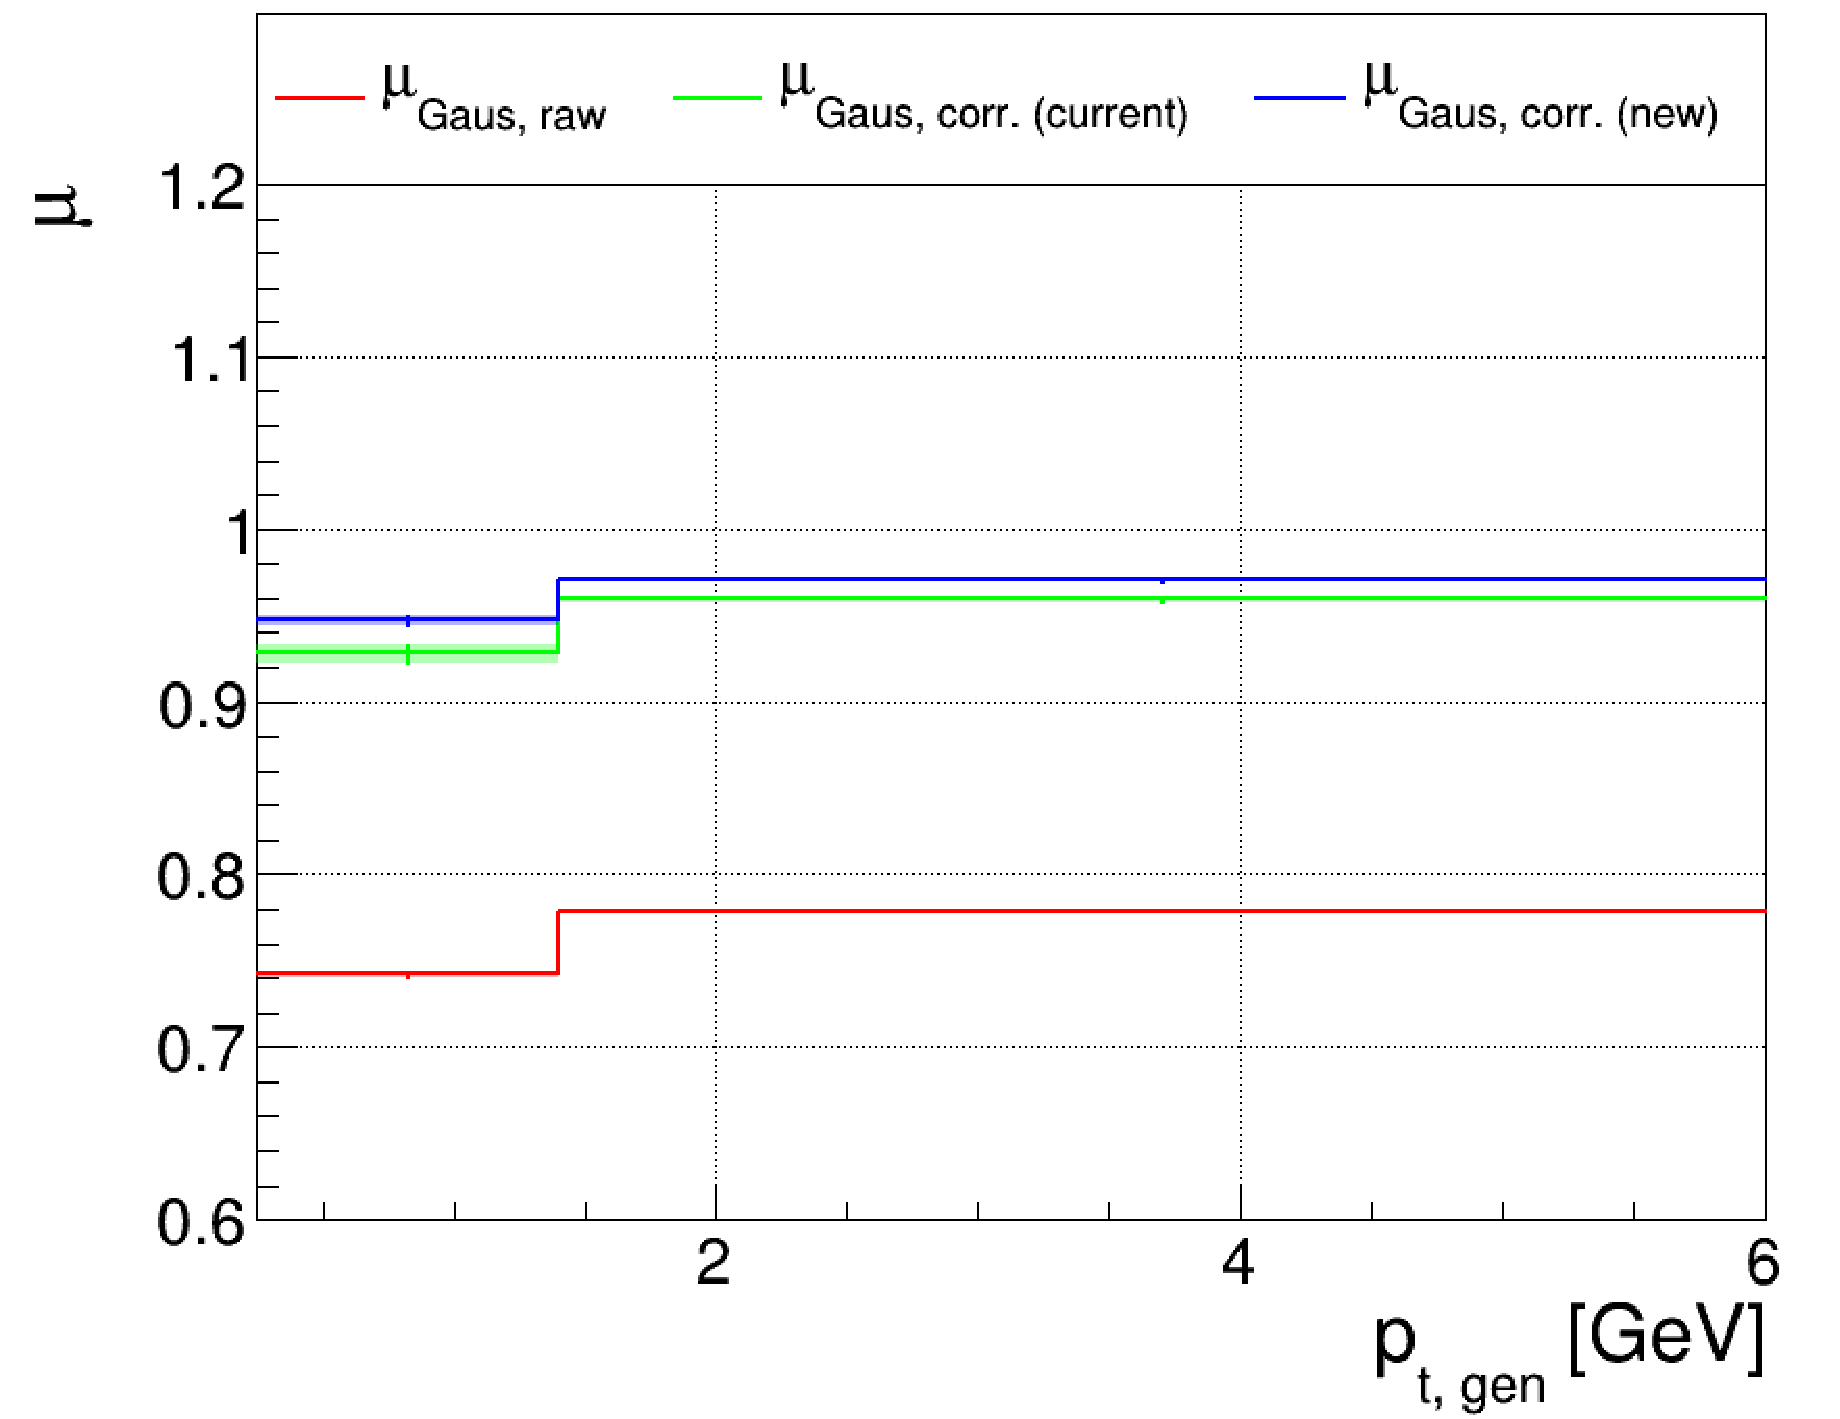
\includegraphics[width=0.495\textwidth]{./plots_pdf/ECAL_plots/plotsNOPU/EB/ZS/pdf/GENPT/EBZS_GENPT_0000_0006_MuOverBins.pdf}
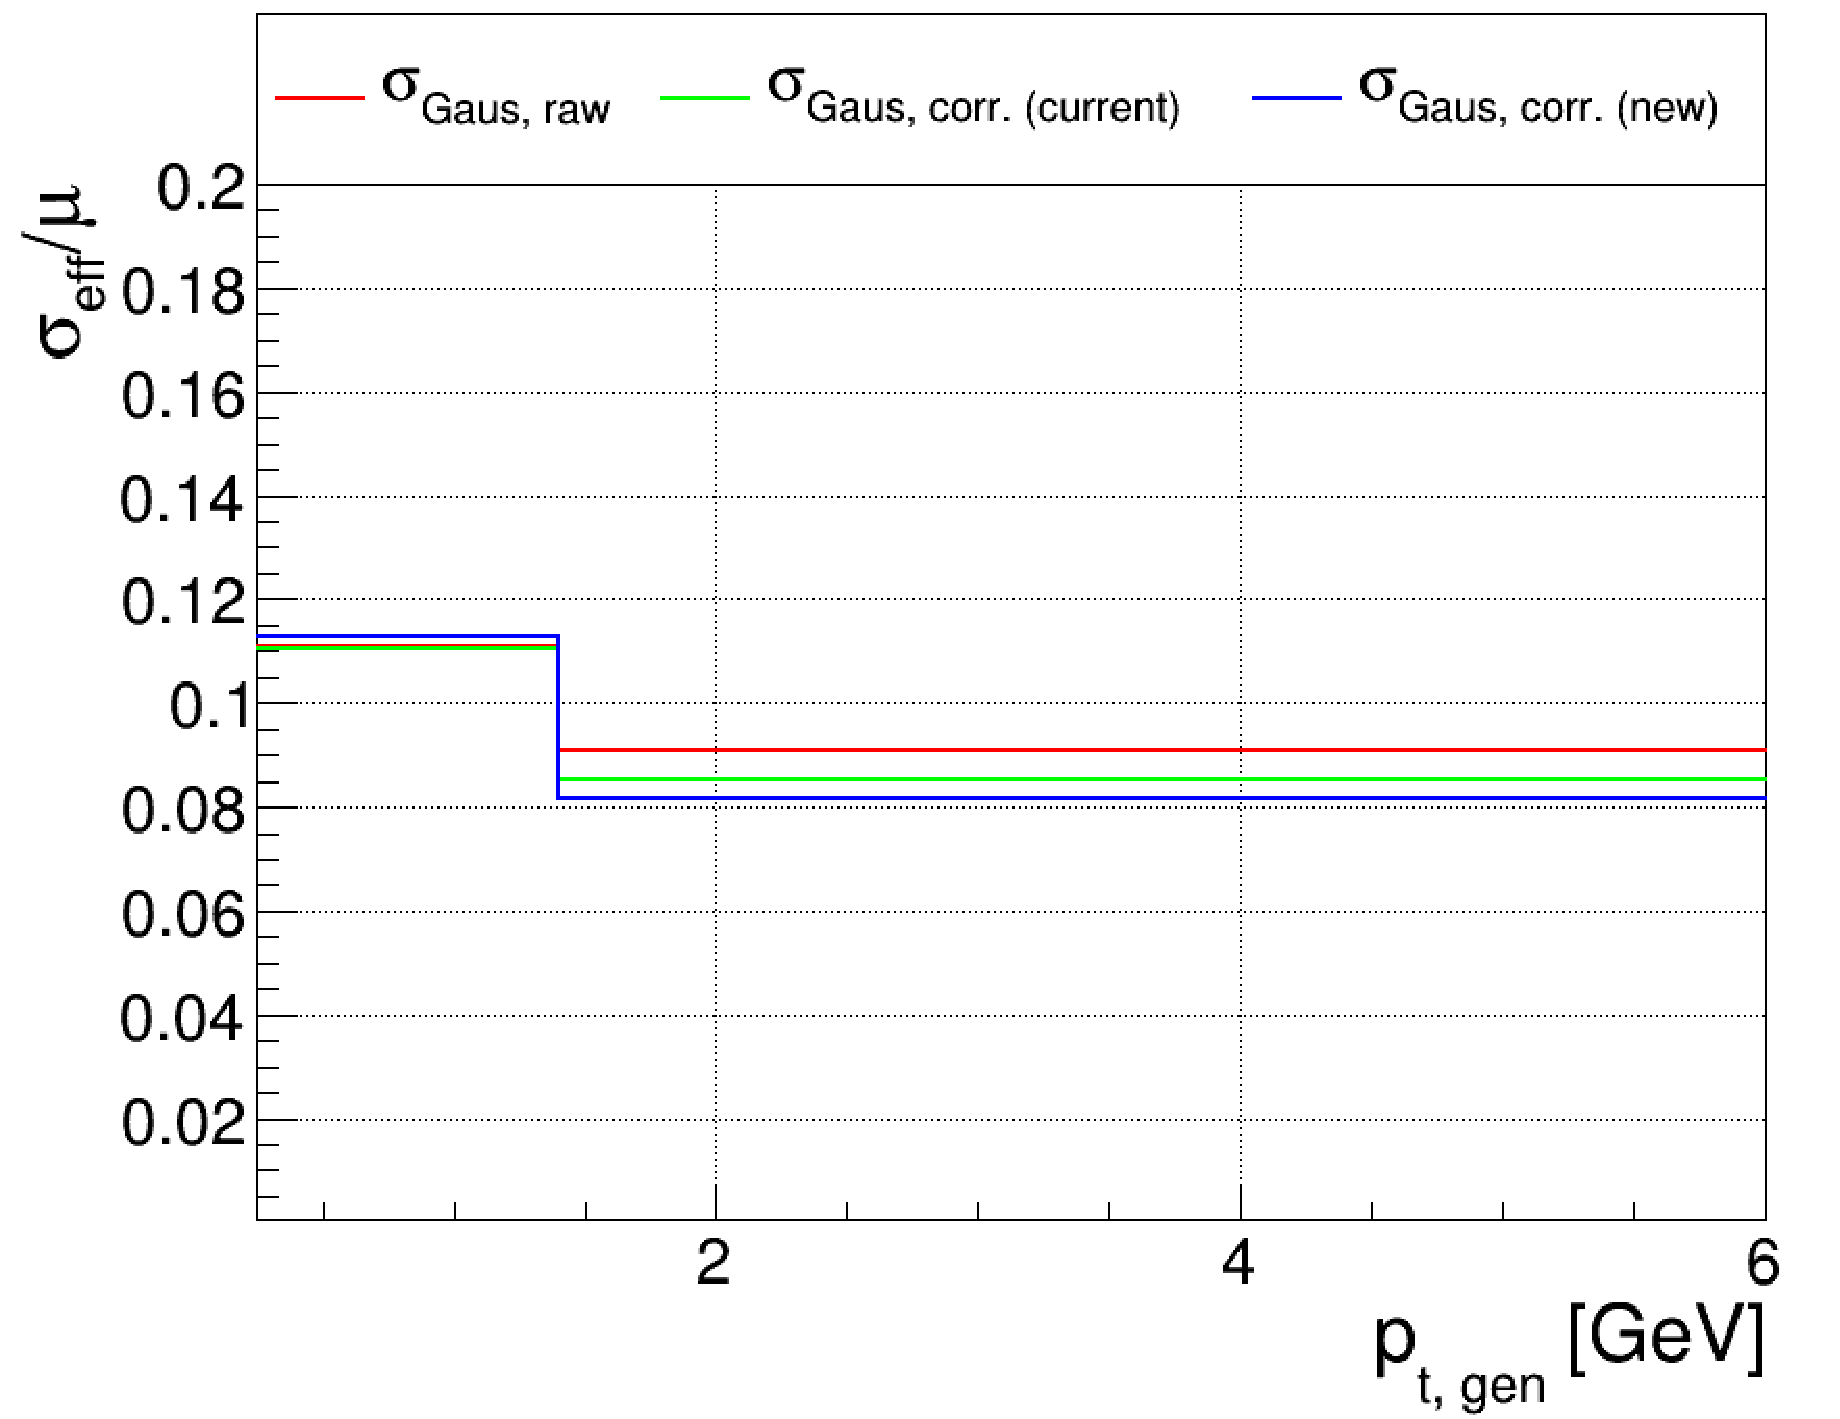
\includegraphics[width=0.495\textwidth]{./plots_pdf/ECAL_plots/plotsNOPU/EB/ZS/pdf/GENPT/EBZS_GENPT_0000_0006_EffSigmaOverBins.pdf}

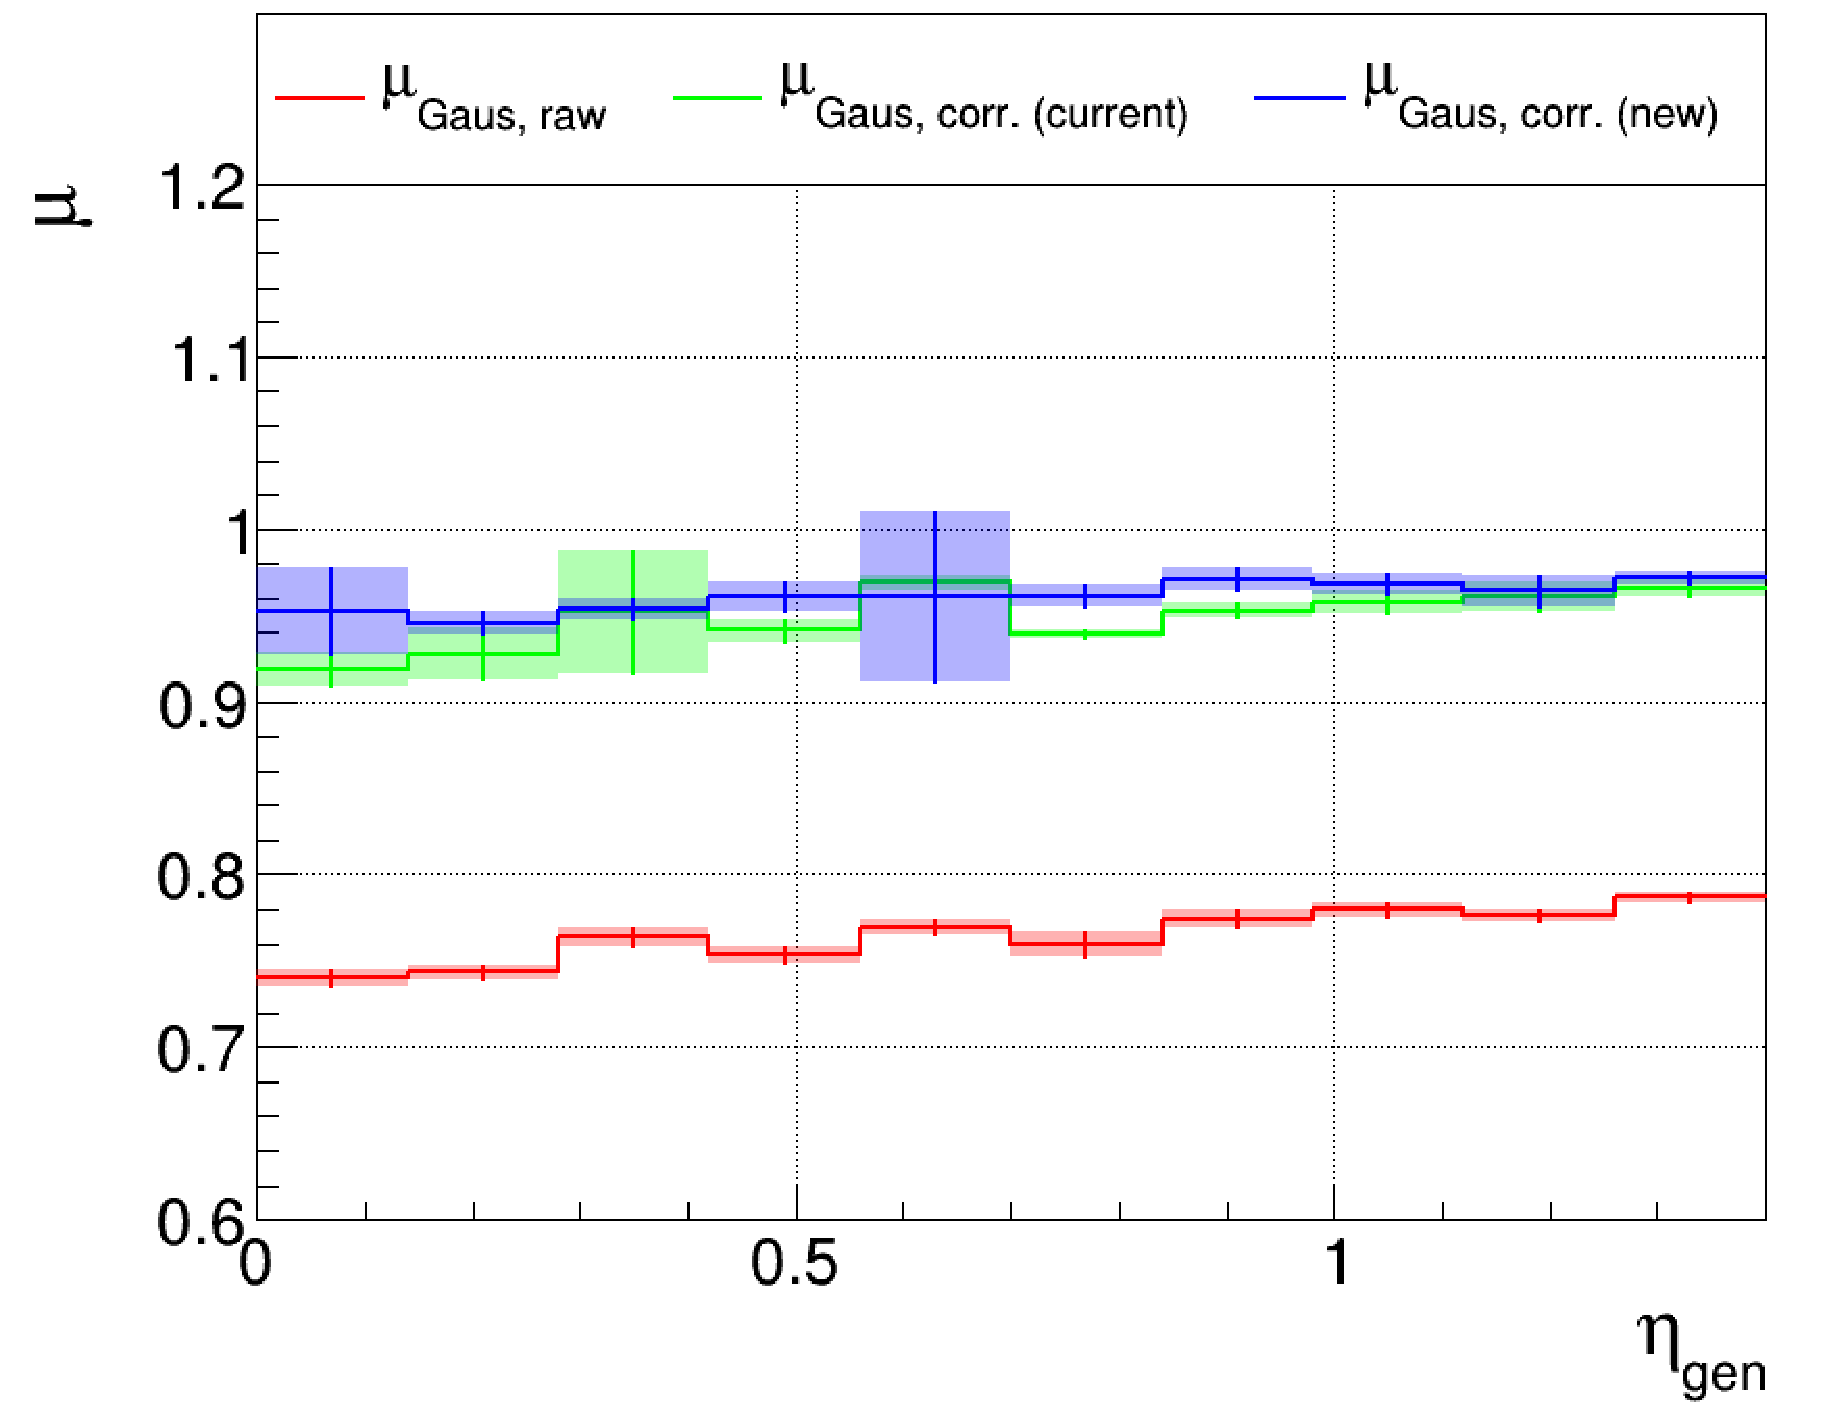
\includegraphics[width=0.495\textwidth]{./plots_pdf/ECAL_plots/plotsNOPU/EB/ZS/pdf/GENETA/EBZS_GENETA_0000_0006_MuOverBins.pdf}
\includegraphics[width=0.495\textwidth]{./plots_pdf/ECAL_plots/plotsNOPU/EB/ZS/pdf/GENETA/EBZS_GENETA_0000_0006_EffSigmaOverBins.pdf}
\caption[]{EB - ZS Readout \pt 0--6\GeV.}
\end{figure}

%% \begin{figure}
%% \includegraphics[width=0.495\textwidth]{./plots_pdf/ECAL_plots/plotsNOPU/EB/ZS/pdf/GENPT/EBZS_GENPT_0006_0025_MuOverBins.pdf}
%% 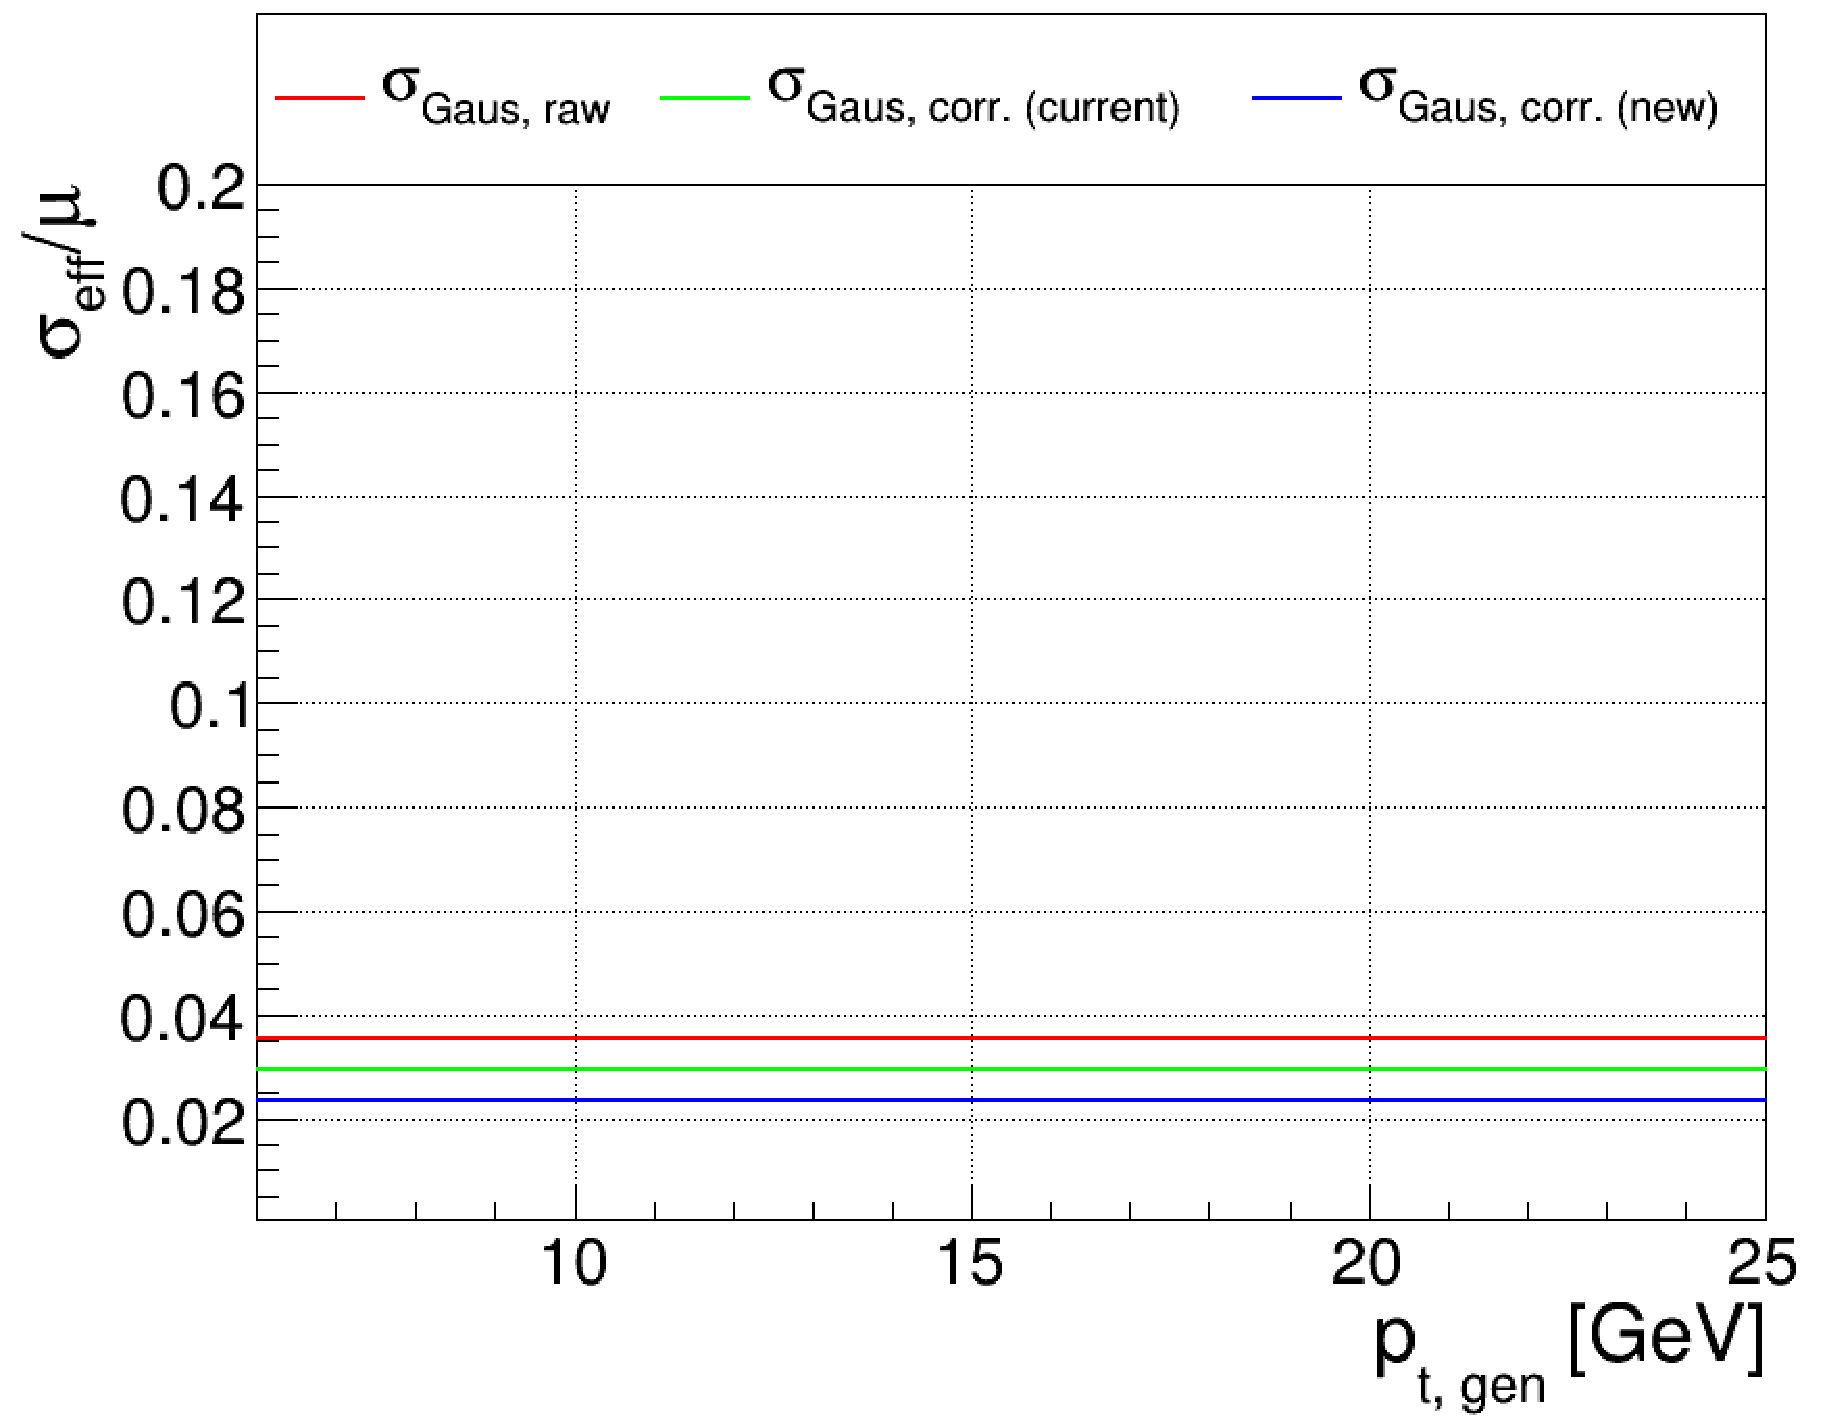
\includegraphics[width=0.495\textwidth]{./plots_pdf/ECAL_plots/plotsNOPU/EB/ZS/pdf/GENPT/EBZS_GENPT_0006_0025_EffSigmaOverBins.pdf}

%% 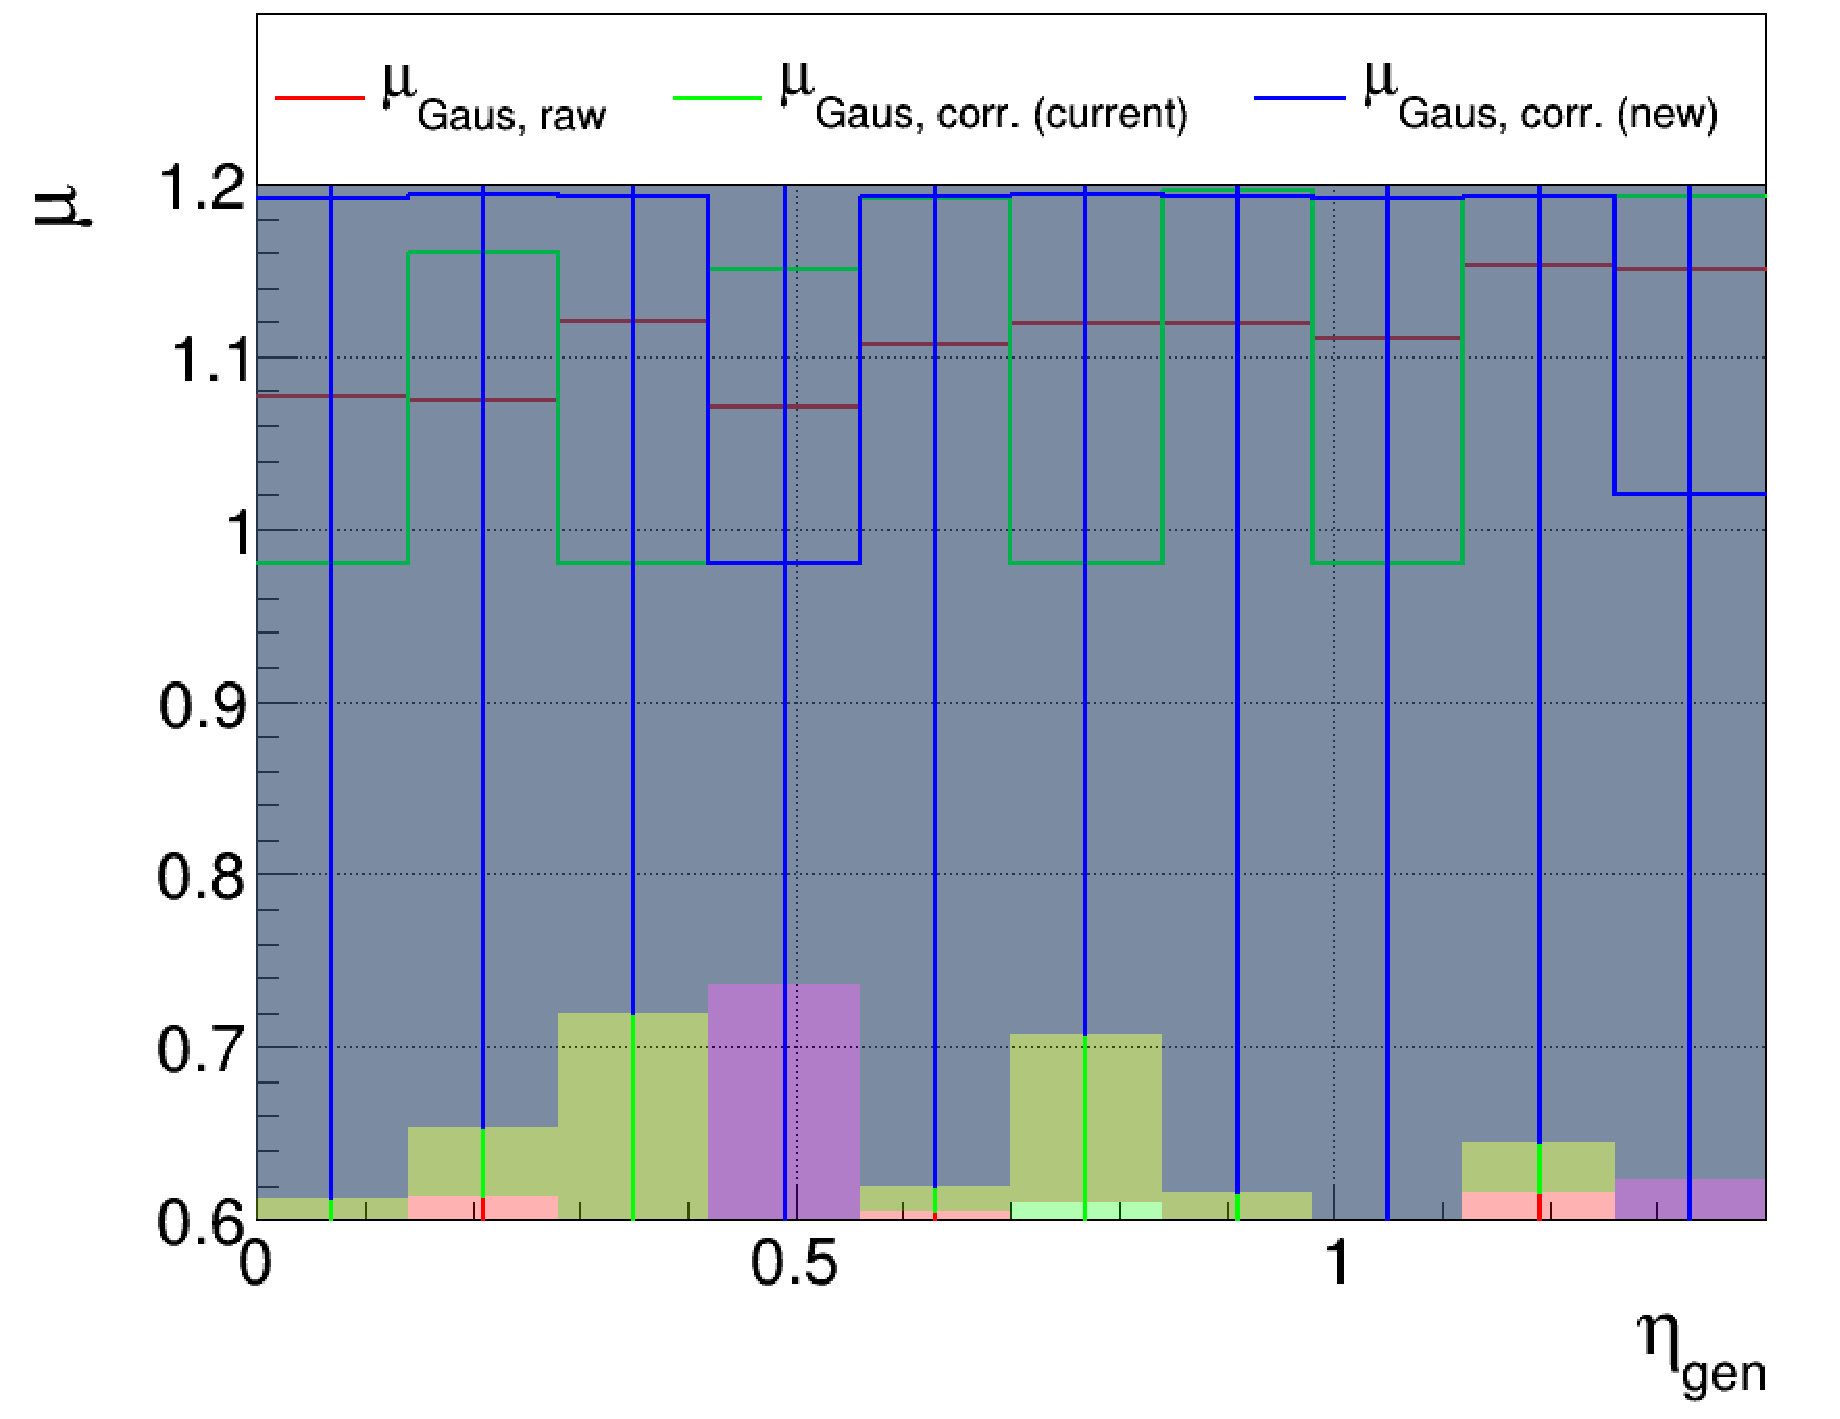
\includegraphics[width=0.495\textwidth]{./plots_pdf/ECAL_plots/plotsNOPU/EB/ZS/pdf/GENETA/EBZS_GENETA_0006_0025_MuOverBins.pdf}
%% 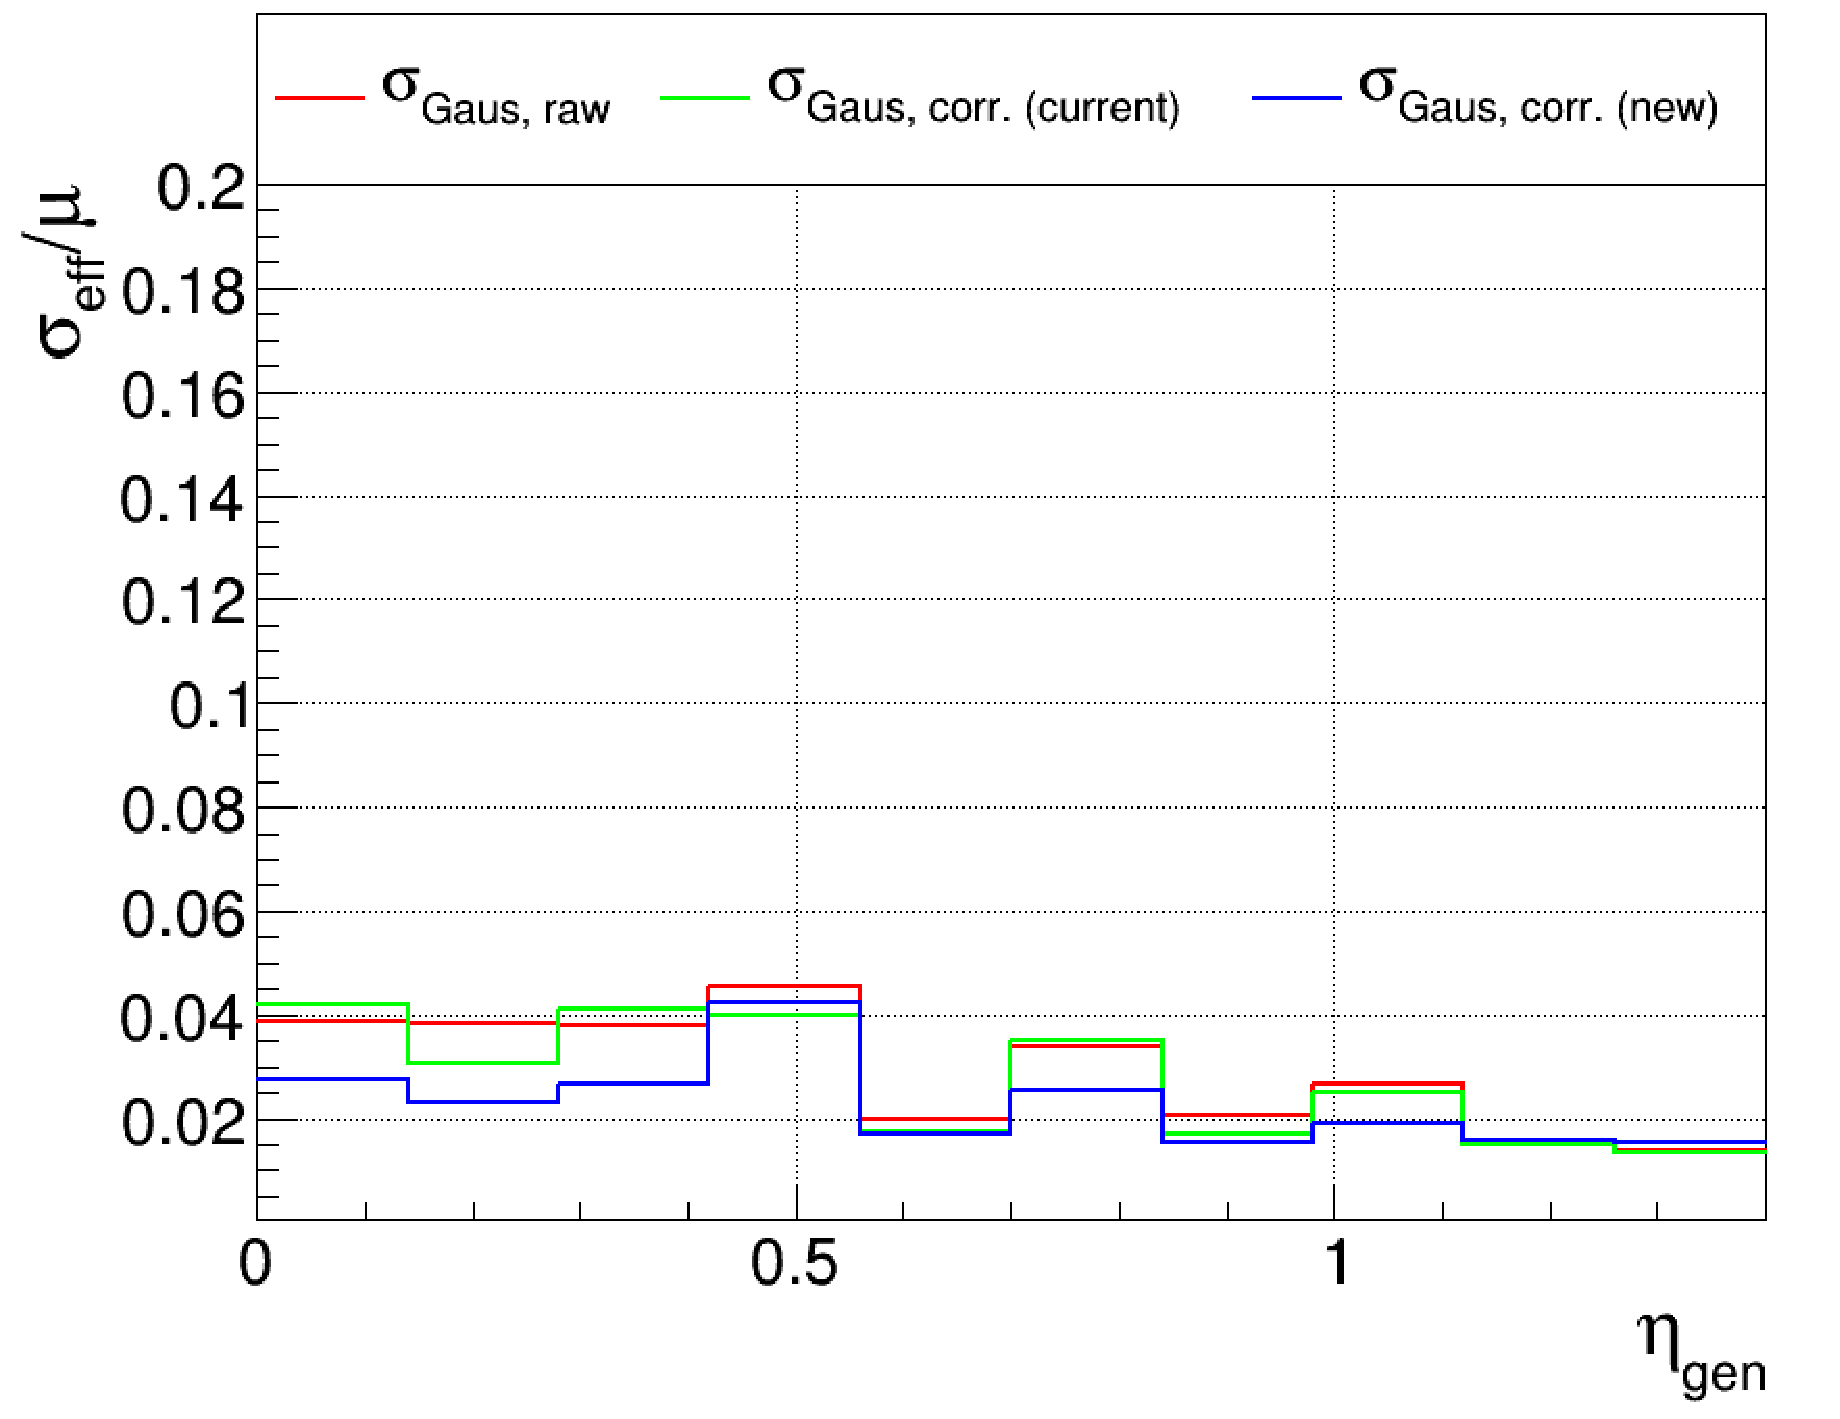
\includegraphics[width=0.495\textwidth]{./plots_pdf/ECAL_plots/plotsNOPU/EB/ZS/pdf/GENETA/EBZS_GENETA_0006_0025_EffSigmaOverBins.pdf}
%% \caption[]{EB - ZS Readout \pt 6-25\GeV}
%% \end{figure}






%\subsubsection{ECAL Endcap}

in EE region:
\begin{figure}
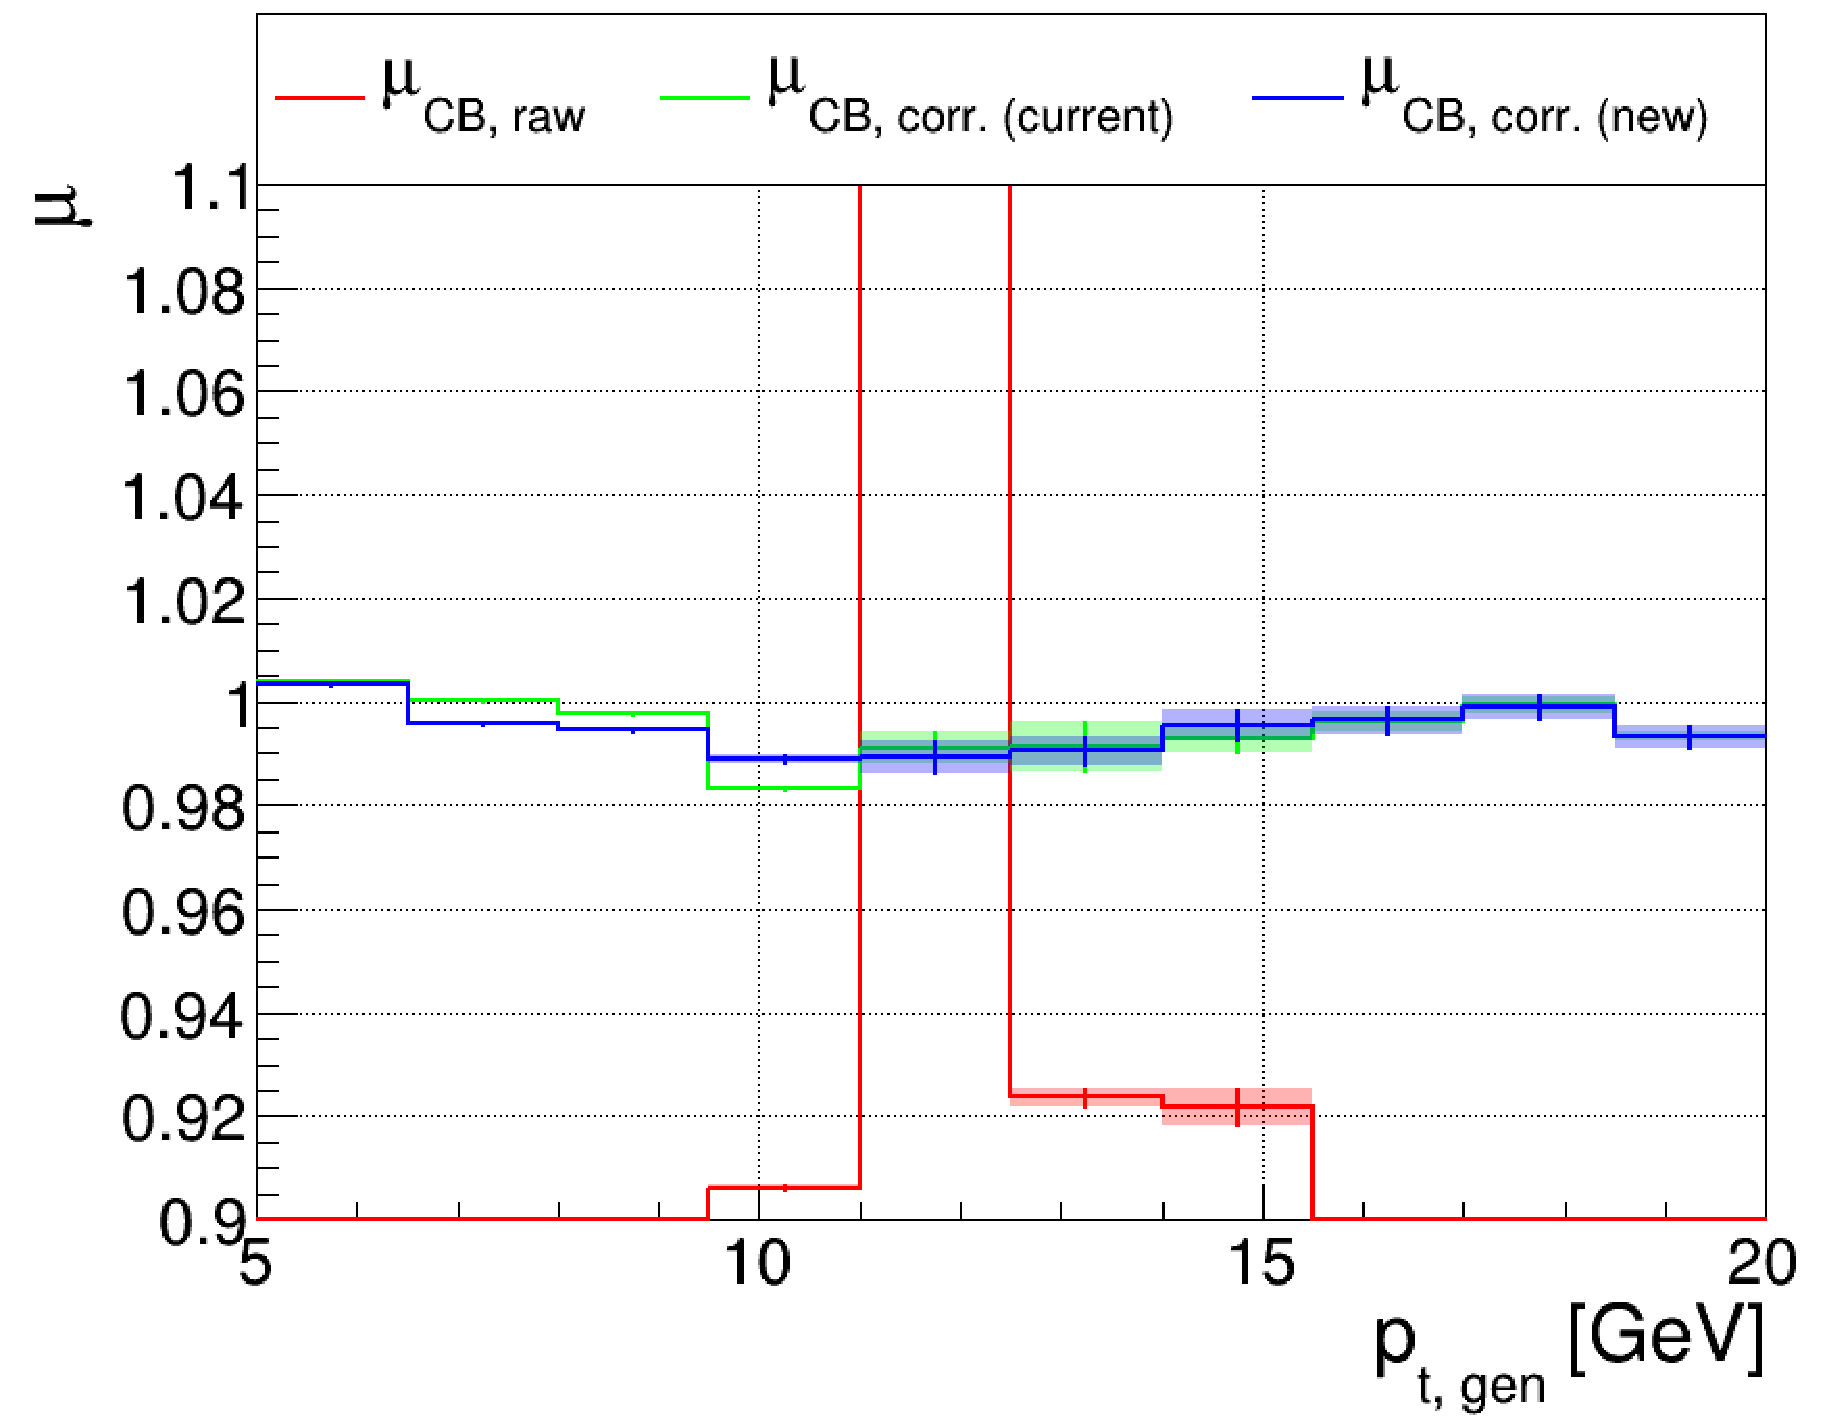
\includegraphics[width=0.495\textwidth]{./plots_pdf/ECAL_plots/plotsNoPU/EE/pdf/FULL/GENPT/EEFULL_GENPT_0005_0020_MuOverBins.pdf}
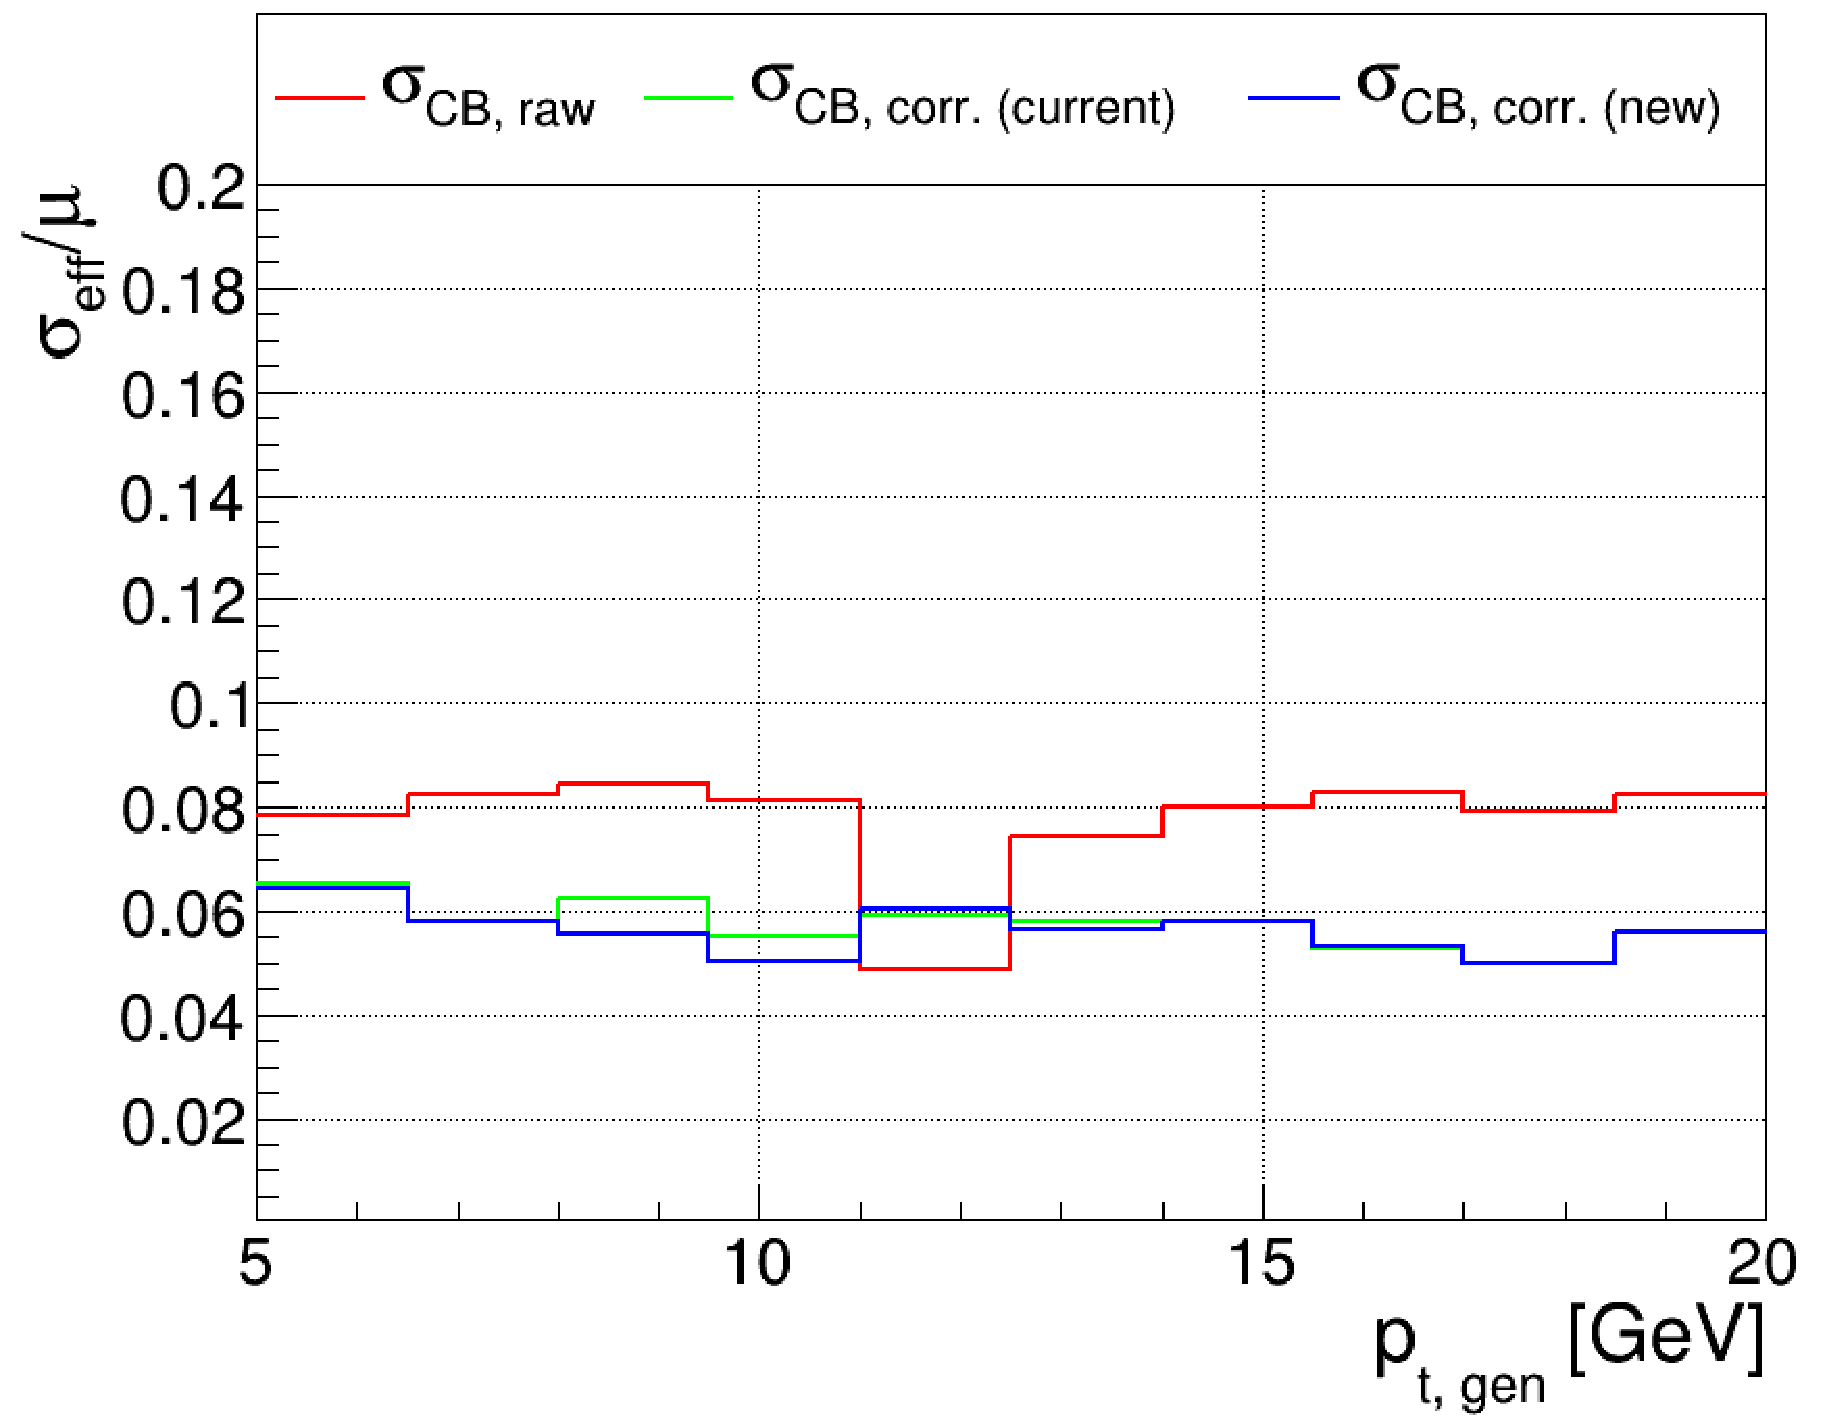
\includegraphics[width=0.495\textwidth]{./plots_pdf/ECAL_plots/plotsNoPU/EE/pdf/FULL/GENPT/EEFULL_GENPT_0005_0020_EffSigmaOverBins.pdf}

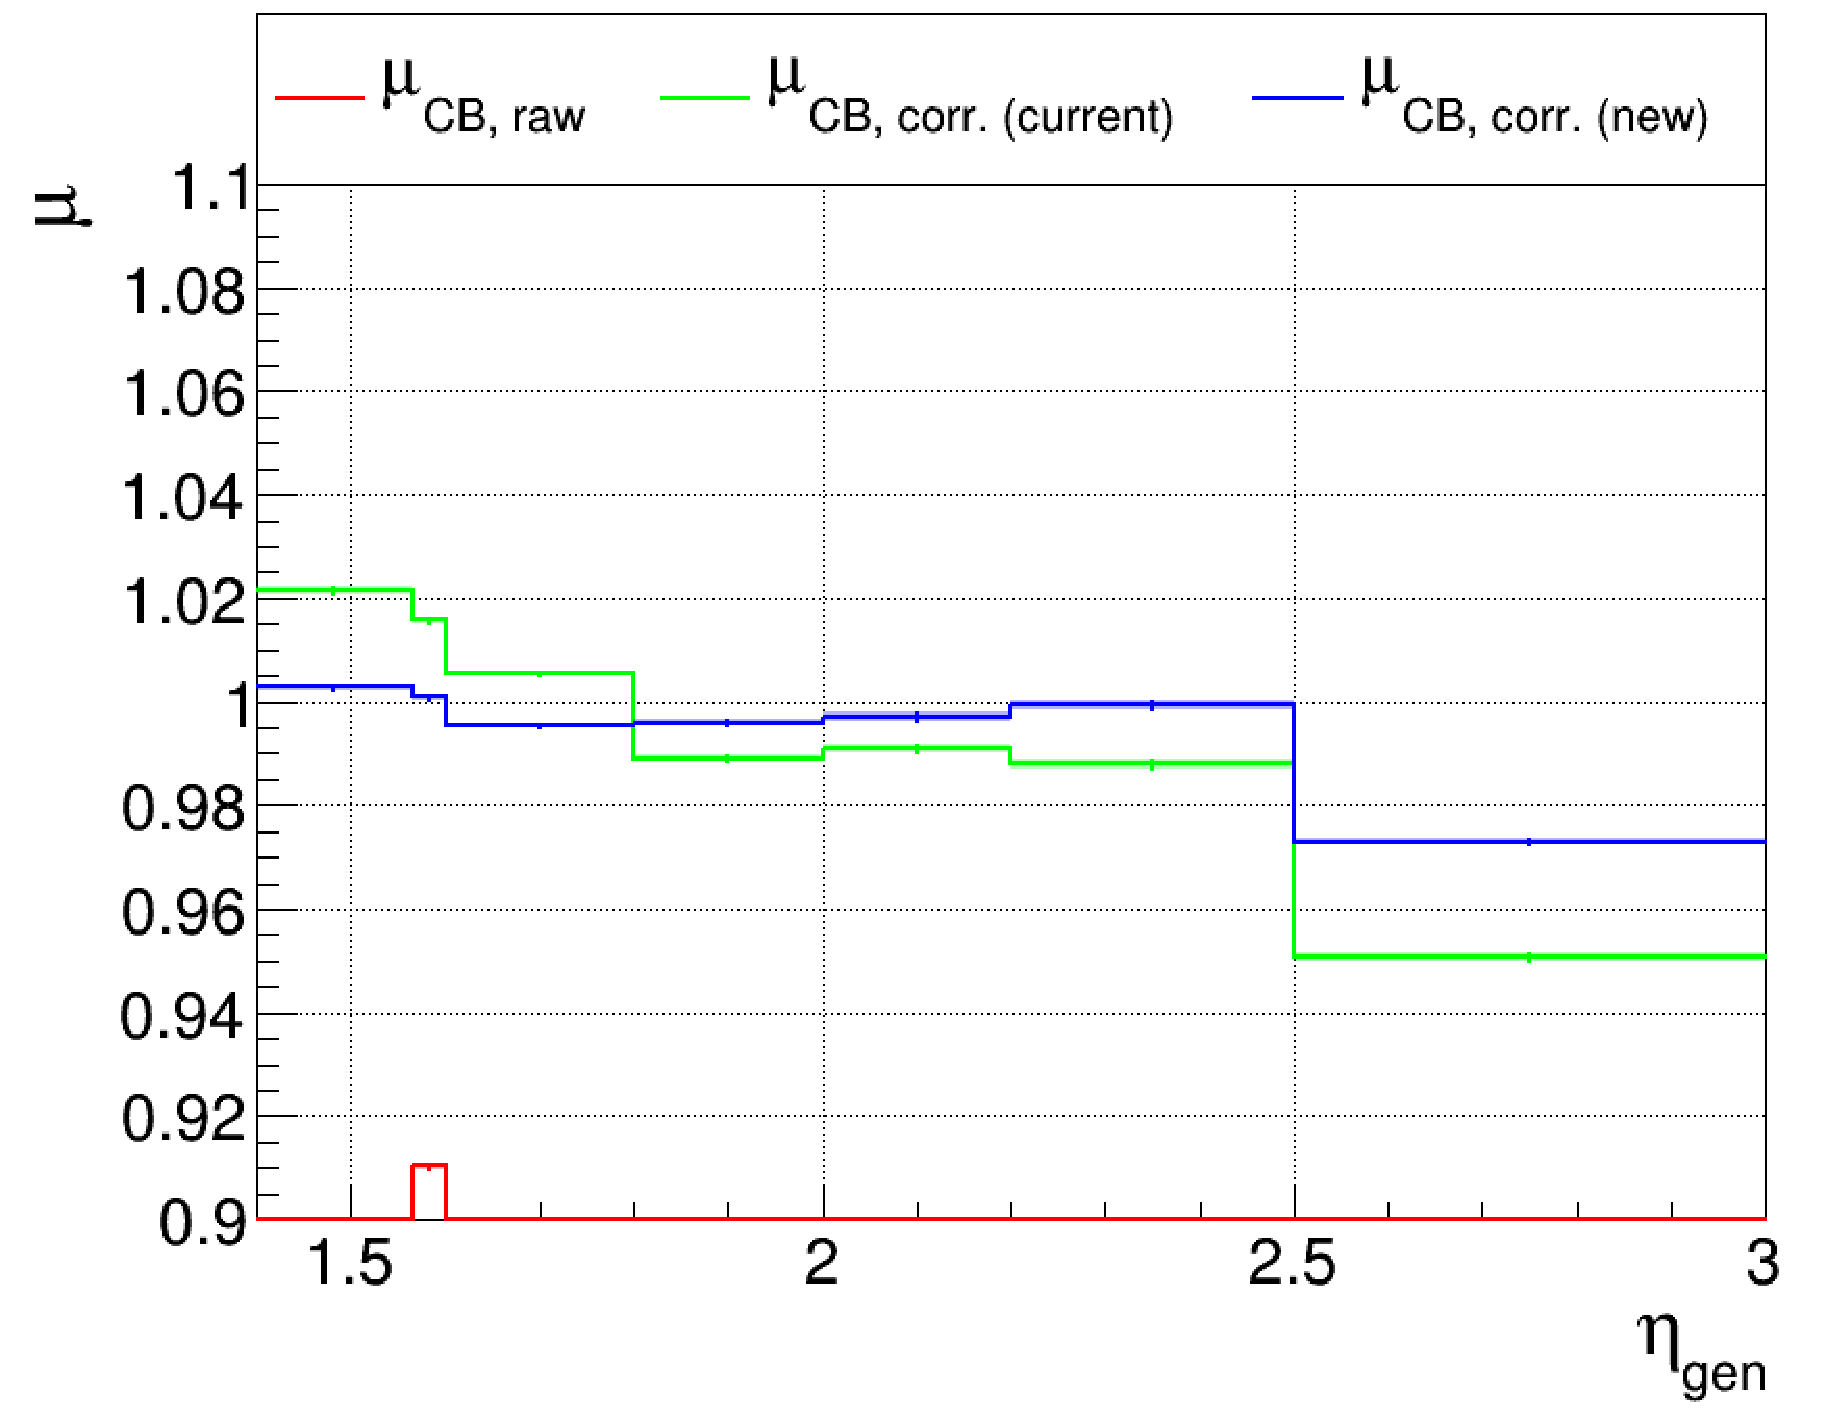
\includegraphics[width=0.495\textwidth]{./plots_pdf/ECAL_plots/plotsNoPU/EE/pdf/FULL/GENETA/EEFULL_GENETA_0005_0020_MuOverBins.pdf}
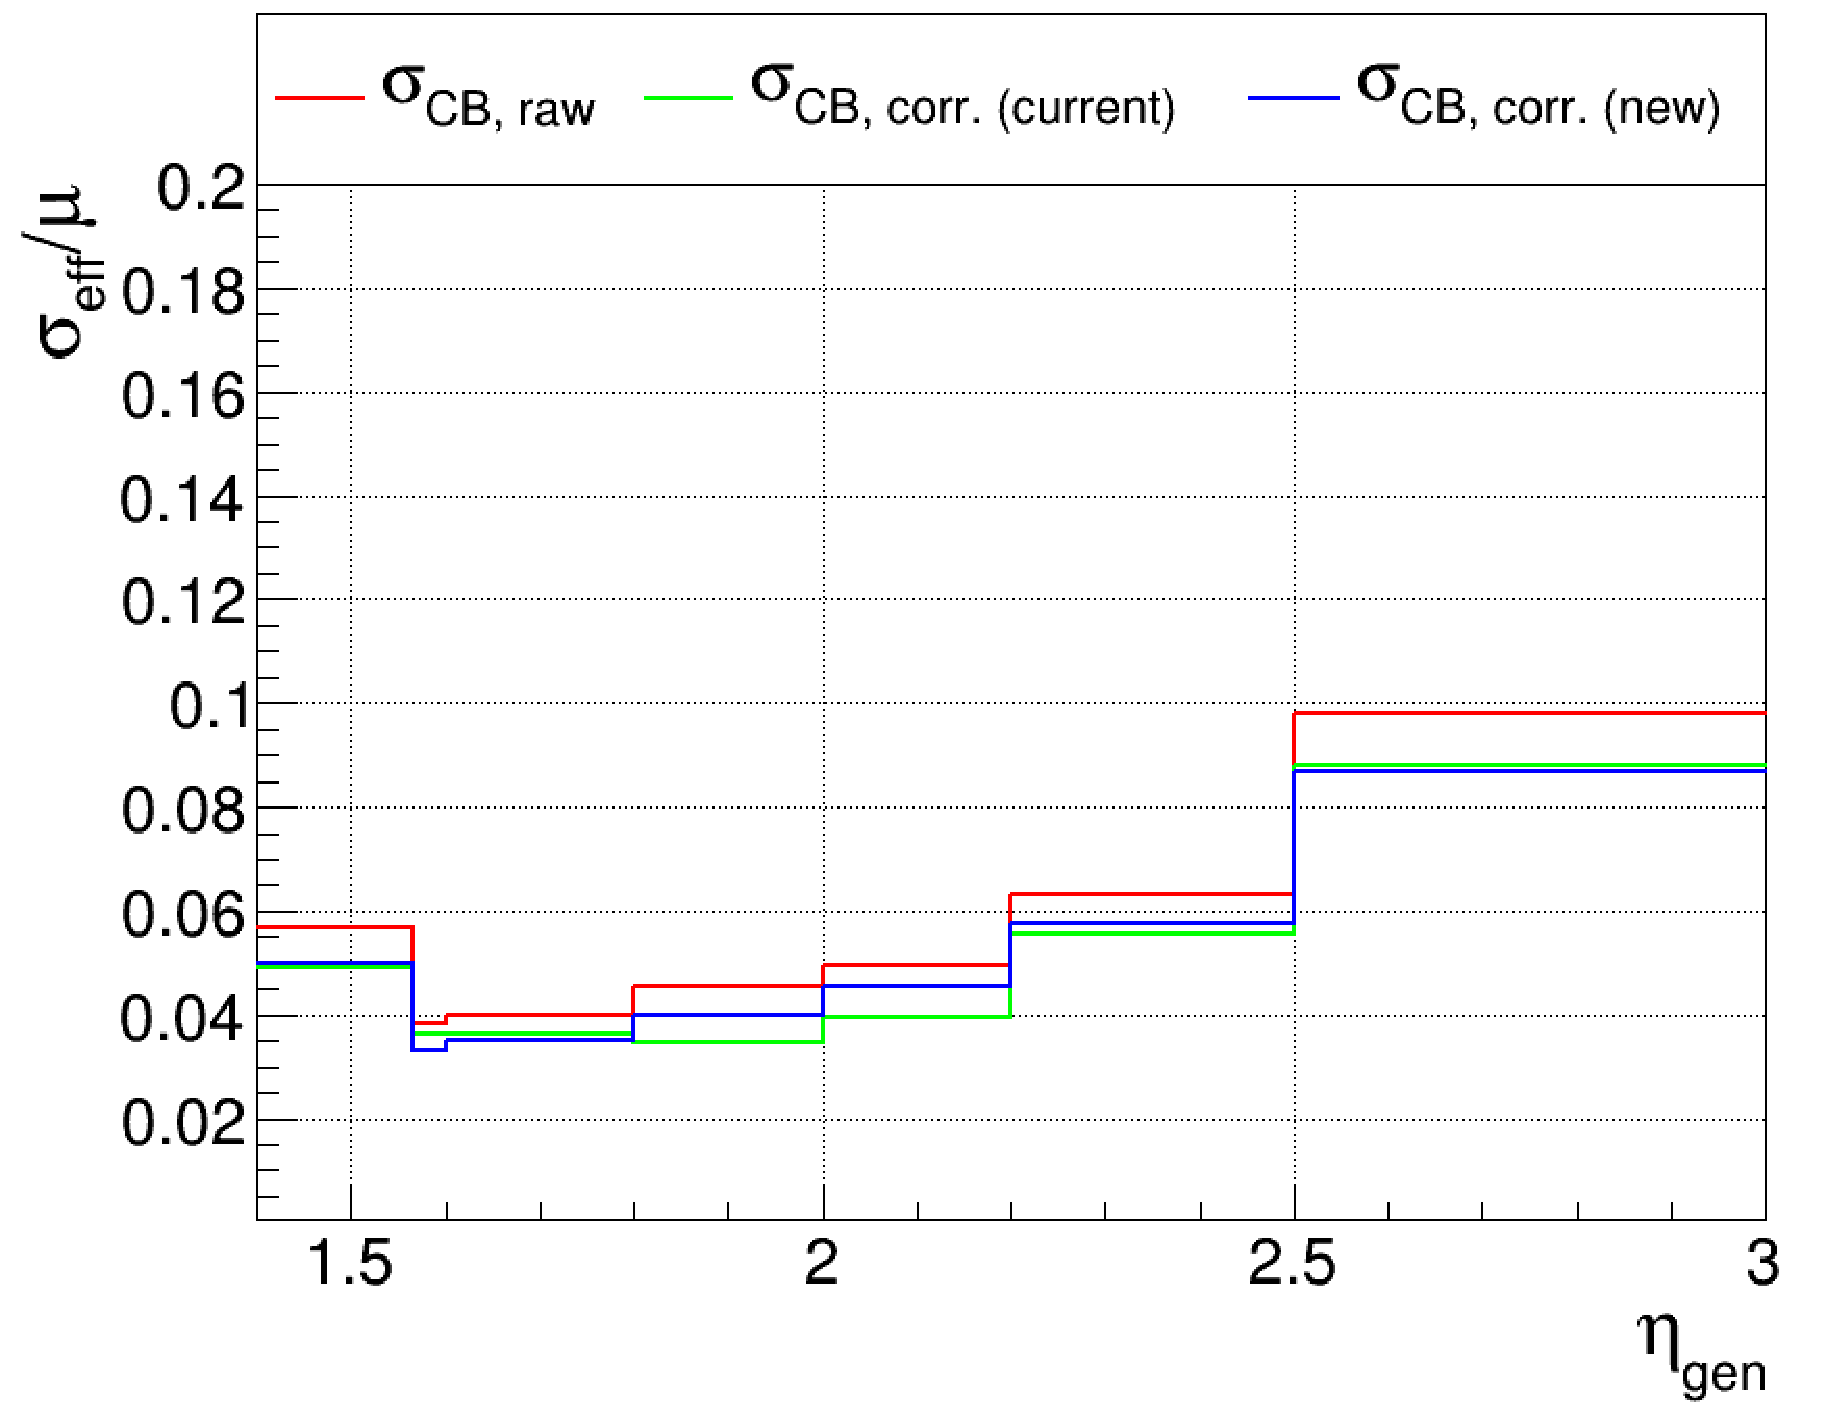
\includegraphics[width=0.495\textwidth]{./plots_pdf/ECAL_plots/plotsNoPU/EE/pdf/FULL/GENETA/EEFULL_GENETA_0005_0020_EffSigmaOverBins.pdf}
\caption{EE - Full Readout \pt 5-20}
%\end{figure}


%\begin{figure}
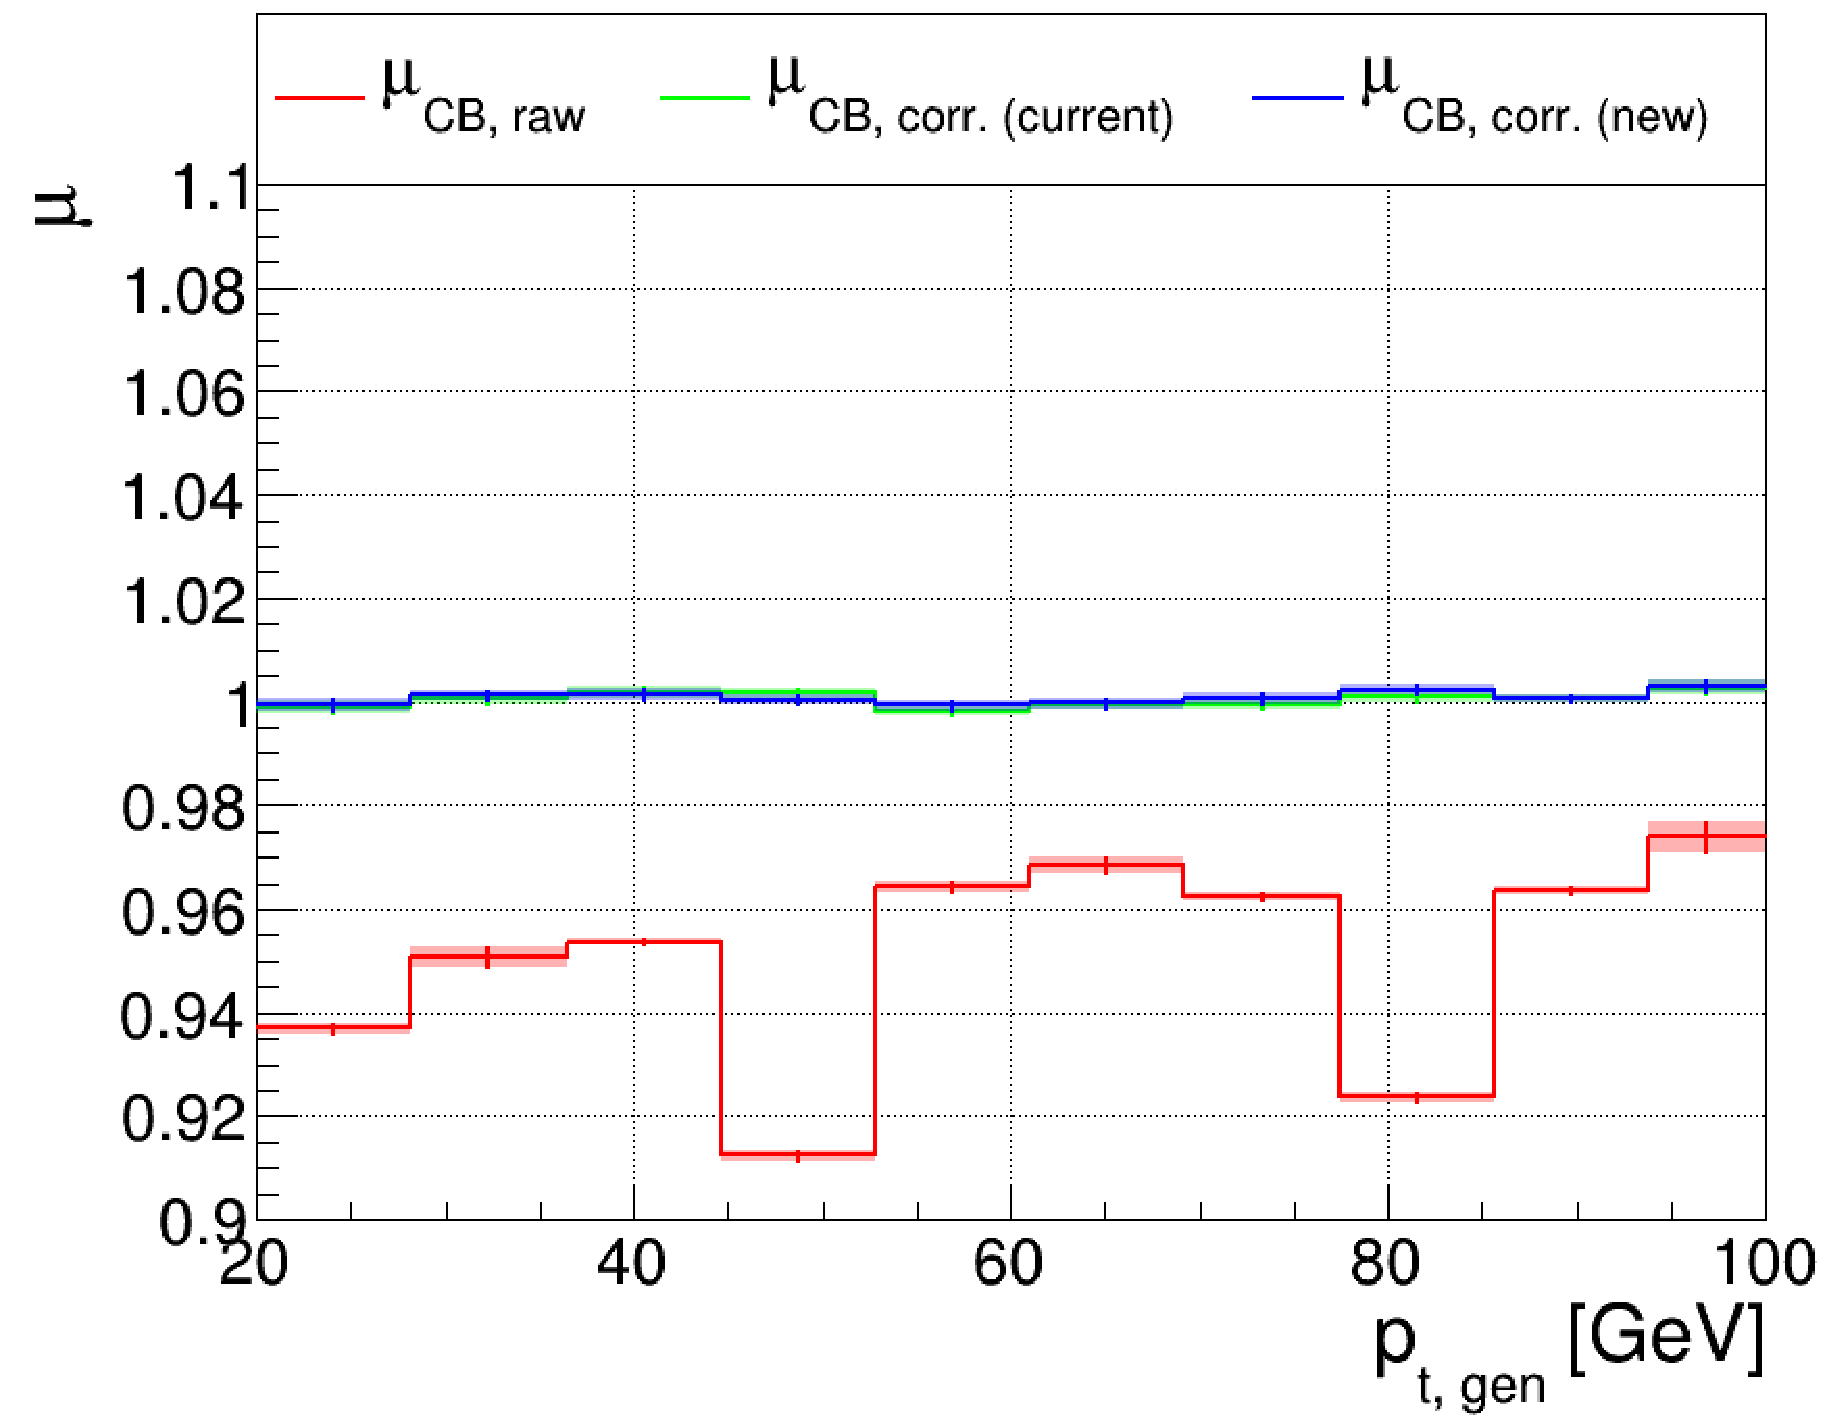
\includegraphics[width=0.495\textwidth]{./plots_pdf/ECAL_plots/plotsNoPU/EE/pdf/FULL/GENPT/EEFULL_GENPT_0020_0100_MuOverBins.pdf}
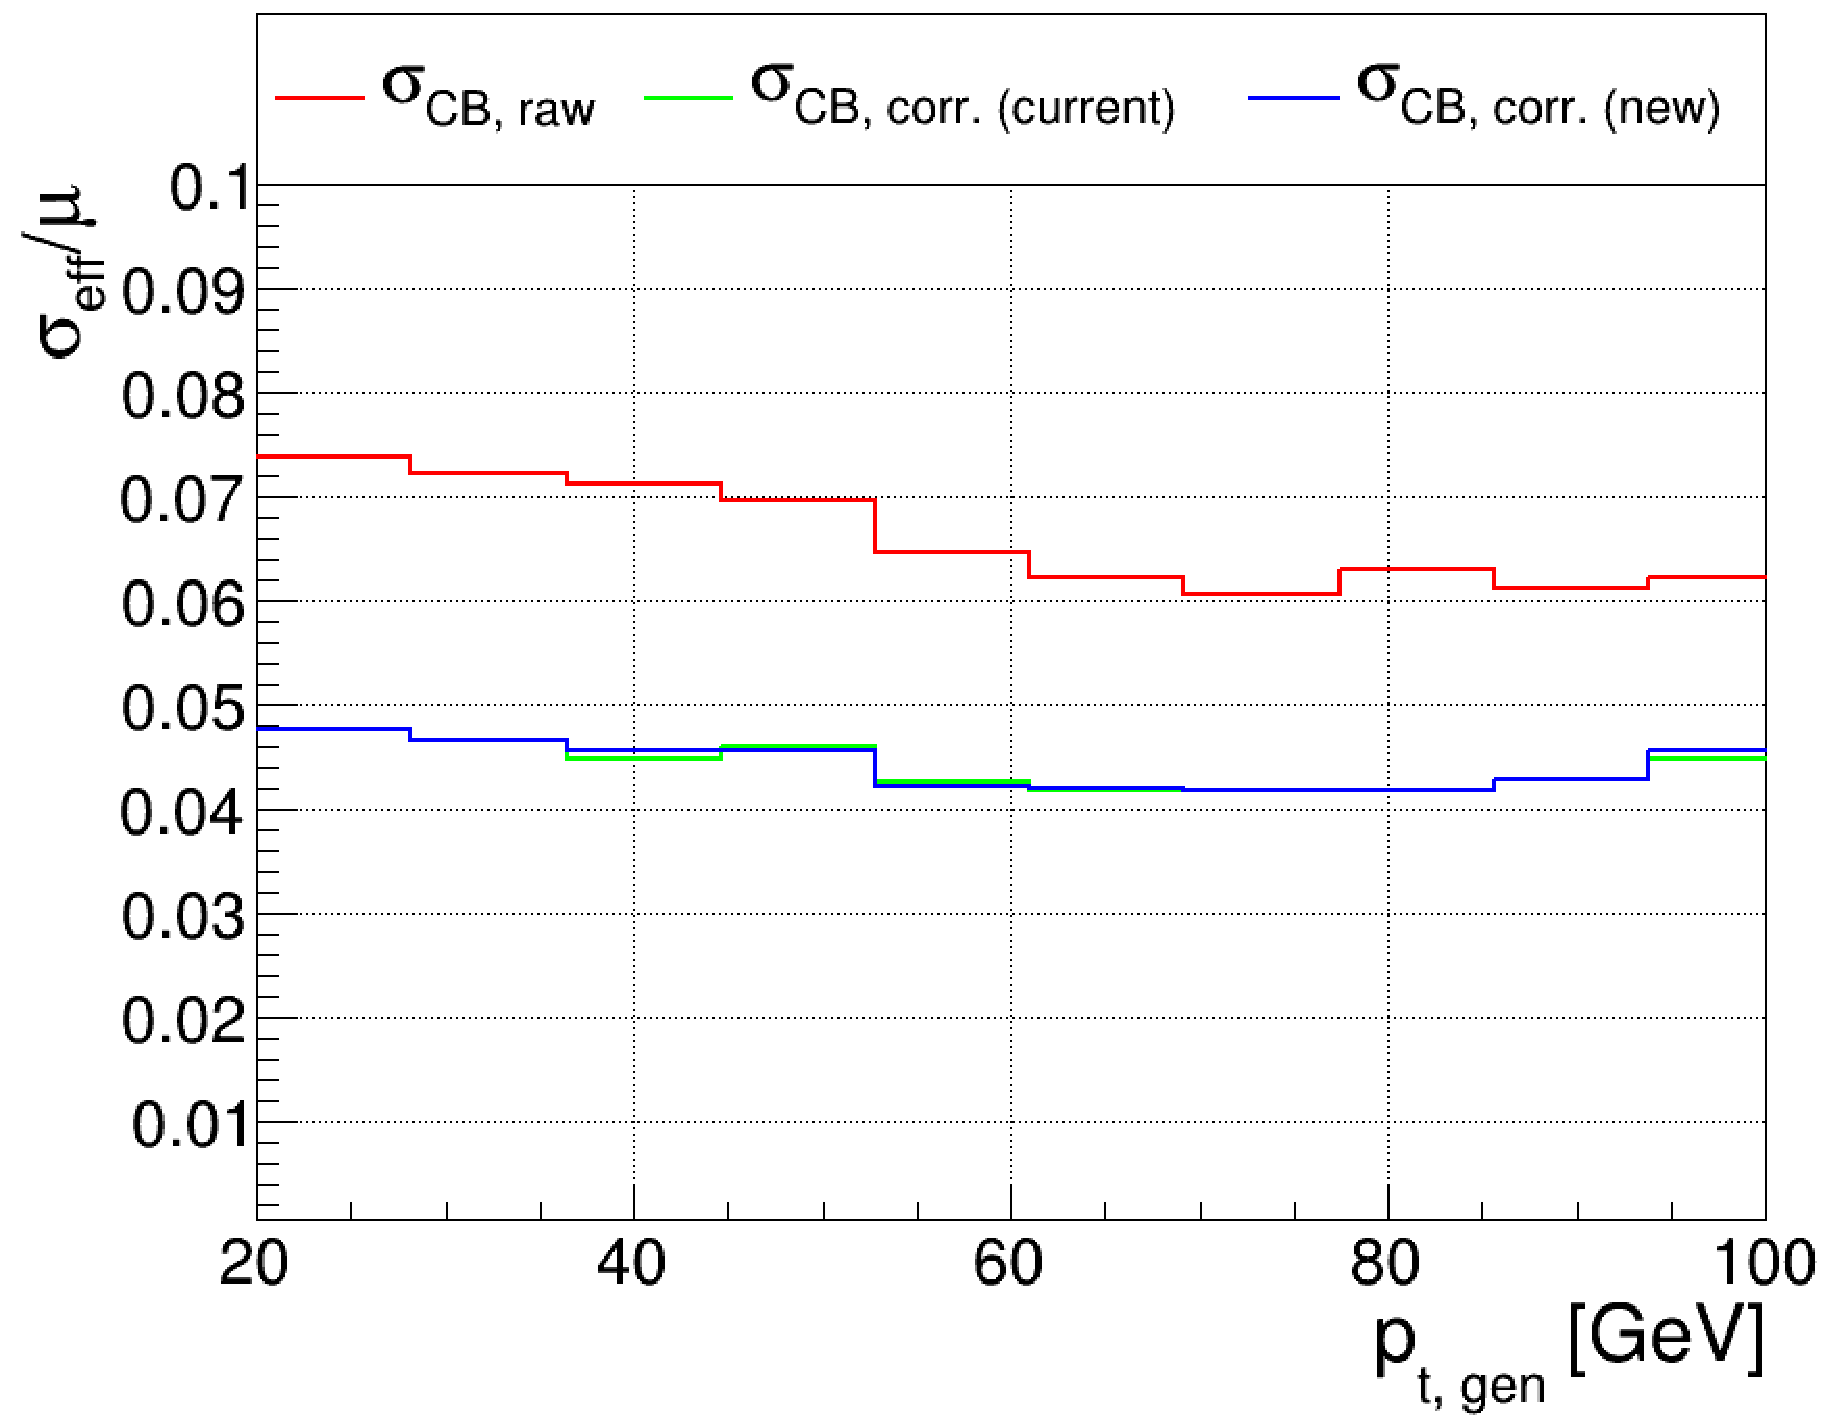
\includegraphics[width=0.495\textwidth]{./plots_pdf/ECAL_plots/plotsNoPU/EE/pdf/FULL/GENPT/EEFULL_GENPT_0020_0100_EffSigmaOverBins.pdf}

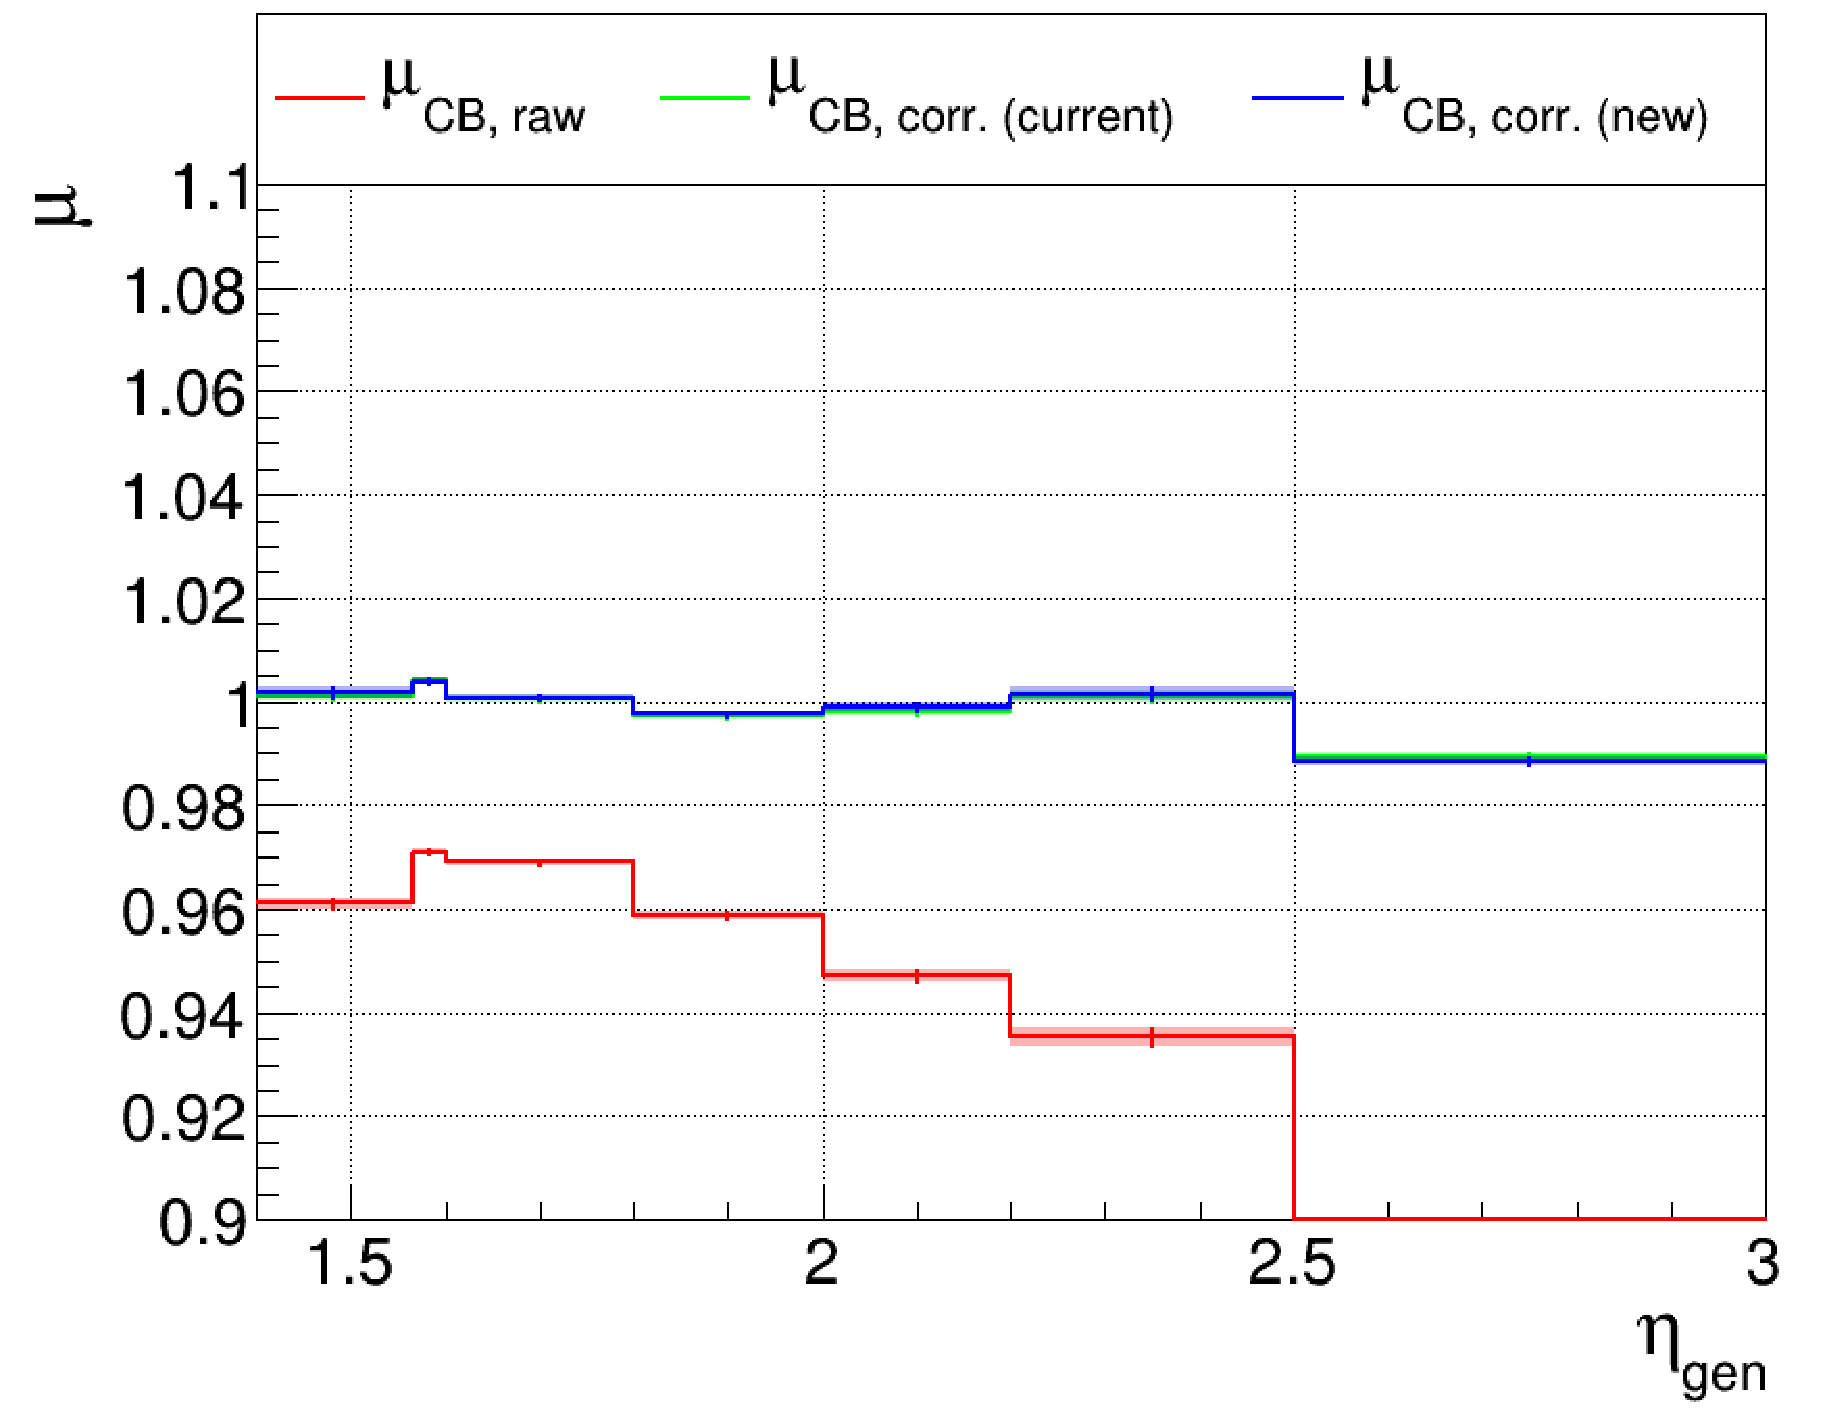
\includegraphics[width=0.495\textwidth]{./plots_pdf/ECAL_plots/plotsNoPU/EE/pdf/FULL/GENETA/EEFULL_GENETA_0020_0100_MuOverBins.pdf}
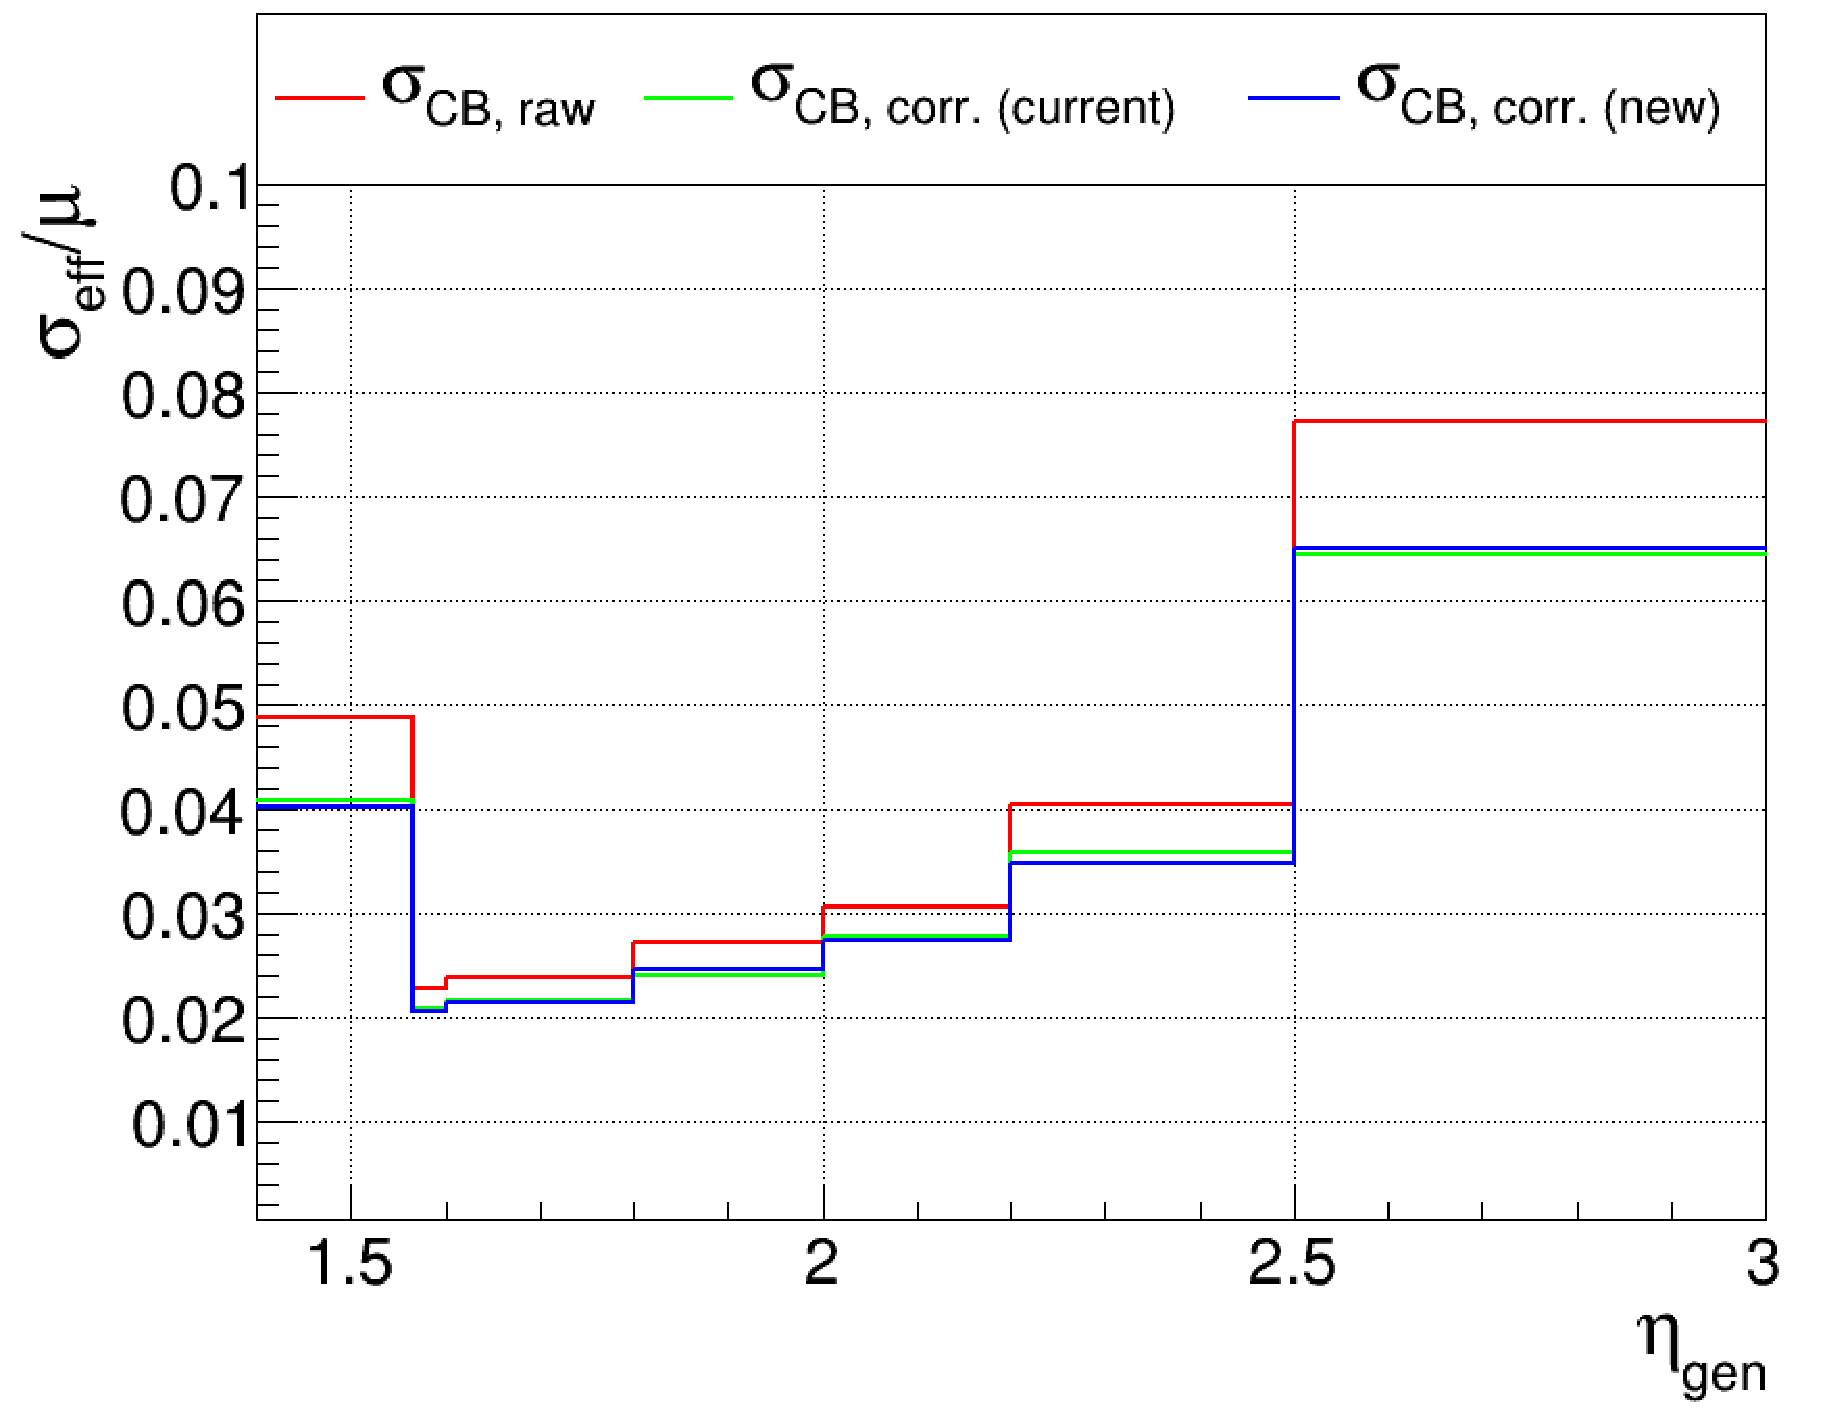
\includegraphics[width=0.495\textwidth]{./plots_pdf/ECAL_plots/plotsNoPU/EE/pdf/FULL/GENETA/EEFULL_GENETA_0020_0100_EffSigmaOverBins.pdf}
\caption{EE - Full Readout \pt 20-100}
\end{figure}


\begin{figure}
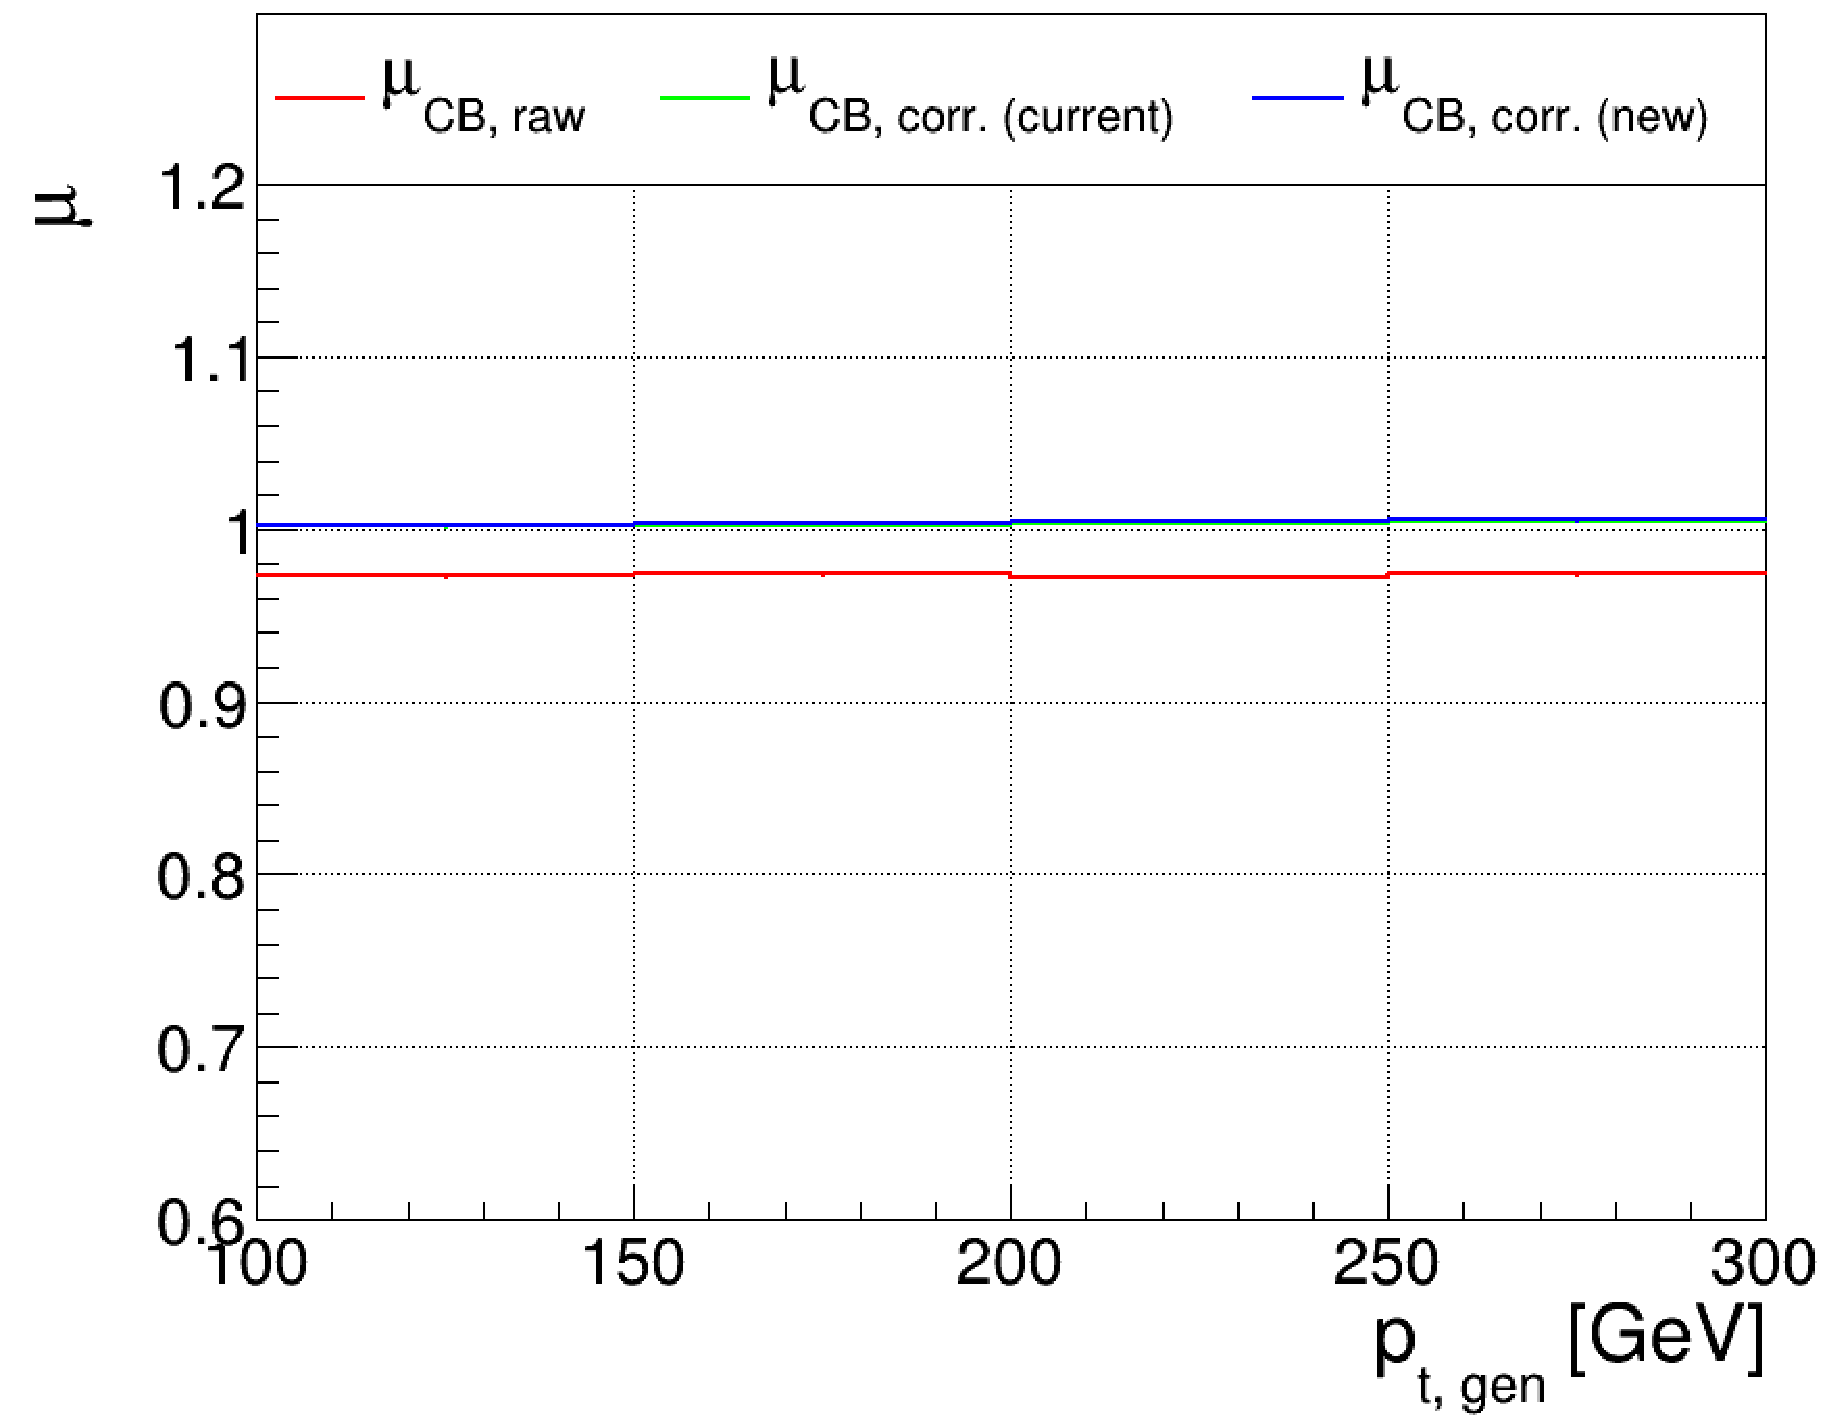
\includegraphics[width=0.495\textwidth]{./plots_pdf/ECAL_plots/plotsNoPU/EE/pdf/FULL/GENPT/EEFULL_GENPT_0100_0300_MuOverBins.pdf}
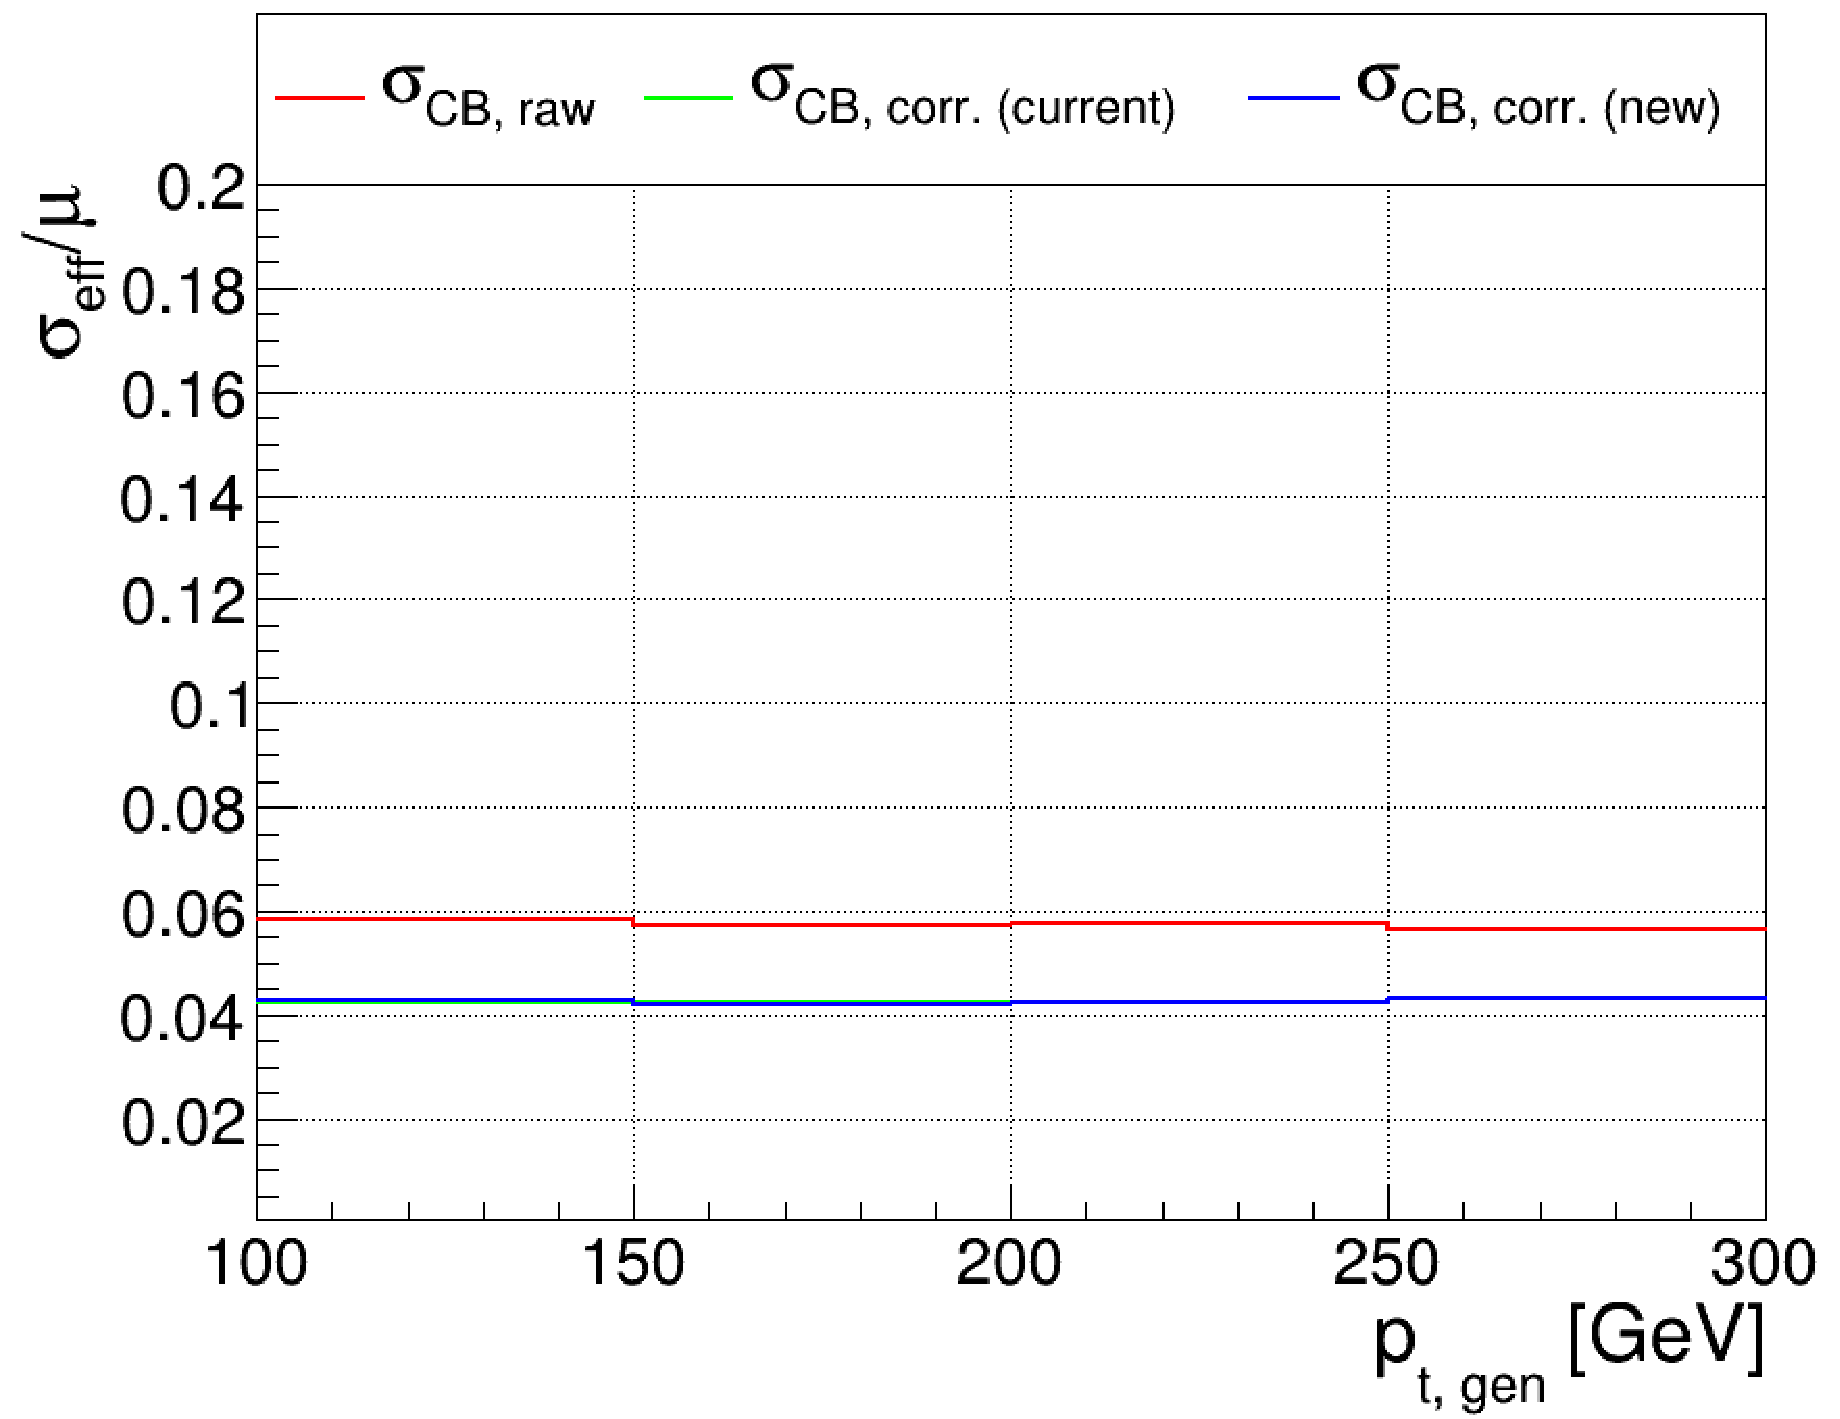
\includegraphics[width=0.495\textwidth]{./plots_pdf/ECAL_plots/plotsNoPU/EE/pdf/FULL/GENPT/EEFULL_GENPT_0100_0300_EffSigmaOverBins.pdf}
%\caption{EE - Full Readout pt 100-300}
%\end{figure}
%\begin{figure}
\includegraphics[width=0.495\textwidth]{./plots_pdf/ECAL_plots/plotsNoPU/EE/pdf/FULL/GENETA/EEFULL_GENETA_0100_0300_MuOverBins.pdf}
\includegraphics[width=0.495\textwidth]{.plots_pdf/ECAL_plots/plotsNoPU/EE/pdf/FULL/GENETA/EEFULL_GENETA_0100_0300_EffSigmaOverBins.pdf}
\caption{EE - Full Readout \pt 100-300}
\end{figure}





\begin{figure}
\includegraphics[width=0.495\textwidth]{./plots_pdf/ECAL_plots/plotsNoPU/EE/pdf/ZS/GENPT/EEZS_GENPT_0000_0006_MuOverBins.pdf}
\includegraphics[width=0.495\textwidth]{./plots_pdf/ECAL_plots/plotsNoPU/EE/pdf/ZS/GENPT/EEZS_GENPT_0000_0006_EffSigmaOverBins.pdf}

\includegraphics[width=0.495\textwidth]{./plots_pdf/ECAL_plots/plotsNoPU/EE/pdf/ZS/GENETA/EEZS_GENETA_0000_0006_MuOverBins.pdf}
\includegraphics[width=0.495\textwidth]{./plots_pdf/ECAL_plots/plotsNoPU/EE/pdf/ZS/GENETA/EEZS_GENETA_0000_0006_EffSigmaOverBins.pdf}
\caption[$\mu$ ($\sigma_\mathrm{eff}$) vs \pt of PF ECAL cluster - EE ZS readout NoPU scenario]{Mean response (resolution) defined by Raw PF ECAL clusters (red), the calibration derived earlier in Ru\
n3 based on 126X (green), and the new correction from 2024 simulation sample based on 133X (blue).\pt 0--6\GeV in EE region ZS Readout NOPU scenario.}
\end{figure}

%% %\begin{figure}
%% \includegraphics[width=0.495\textwidth]{./plots_pdf/ECAL_plots/plotsNoPU/EE/pdf/ZS/GENPT/EEZS_GENPT_0006_0025_MuOverBins.pdf}
%% \includegraphics[width=0.495\textwidth]{./plots_pdf/ECAL_plots/plotsNoPU/EE/pdf/ZS/GENPT/EEZS_GENPT_0006_0025_EffSigmaOverBins.pdf}
%% %\caption{EE - ZS Readout pt 6-25}
%% %\end{figure}
%% %\begin{figure}
%% \includegraphics[width=0.495\textwidth]{./plots_pdf/ECAL_plots/plotsNoPU/EE/pdf/ZS/GENETA/EEZS_GENETA_0006_0025_MuOverBins.pdf}
%% %\includegraphics[width=0.495\textwidth]{./ECAL_plots/plotsNoPU/EE/pdf/ZS/GENETA/EEZS_GENETA_0006_0025_EffSigmaOverBins.pdf}
%% \caption{EE - ZS Readout \pt 6-25}
%% \end{figure}




\begin{figure}
\includegraphics[width=0.495\textwidth]{./plots_pdf/ECAL_plots/plotsPU/EE/FULL/pdf/GENPT/EEFULL_GENPT_0005_0020_MuOverBins.pdf}
\includegraphics[width=0.495\textwidth]{./plots_pdf/ECAL_plots/plotsPU/EE/FULL/pdf/GENPT/EEFULL_GENPT_0005_0020_EffSigmaOverBins.pdf}
\includegraphics[width=0.495\textwidth]{./plots_pdf/ECAL_plots/plotsPU/EE/FULL/pdf/GENPT/EEFULL_GENPT_0020_0100_MuOverBins.pdf}
\includegraphics[width=0.495\textwidth]{./plots_pdf/ECAL_plots/plotsPU/EE/FULL/pdf/GENPT/EEFULL_GENPT_0020_0100_EffSigmaOverBins.pdf}
\includegraphics[width=0.495\textwidth]{./plots_pdf/ECAL_plots/plotsPU/EE/FULL/pdf/GENPT/EEFULL_GENPT_0100_0300_MuOverBins.pdf}
\includegraphics[width=0.495\textwidth]{./plots_pdf/ECAL_plots/plotsPU/EE/FULL/pdf/GENPT/EEFULL_GENPT_0100_0300_EffSigmaOverBins.pdf}

\caption [$\mu$ ($\sigma_\mathrm{eff}$) vs \pt of PF ECAL cluster - EE full readout PU scenario]{Mean response (resolution) defined by Raw PF ECAL clusters (red), the calibration derived earlier in Ru\
n3 based on 126X (green), and the new correction from 2024 simulation sample based on 133X (blue). (top) low \pt, (middle) mid \pt, (bottom) high \pt in EE region full readout PU scenario.}
\label{fig:PU_EEFULL_pt}
\end{figure}


\begin{figure}
\includegraphics[width=0.495\textwidth]{./plots_pdf/ECAL_plots/plotsPU/EE/FULL/pdf/GENETA/EEFULL_GENETA_0005_0020_MuOverBins.pdf}
\includegraphics[width=0.495\textwidth]{./plots_pdf/ECAL_plots/plotsPU/EE/FULL/pdf/GENETA/EEFULL_GENETA_0005_0020_EffSigmaOverBins.pdf}
\includegraphics[width=0.495\textwidth]{./plots_pdf/ECAL_plots/plotsPU/EE/FULL/pdf/GENETA/EEFULL_GENETA_0020_0100_MuOverBins.pdf}
\includegraphics[width=0.495\textwidth]{./plots_pdf/ECAL_plots/plotsPU/EE/FULL/pdf/GENETA/EEFULL_GENETA_0020_0100_EffSigmaOverBins.pdf}
\includegraphics[width=0.495\textwidth]{./plots_pdf/ECAL_plots/plotsPU/EE/FULL/pdf/GENETA/EEFULL_GENETA_0100_0300_MuOverBins.pdf}
\includegraphics[width=0.495\textwidth]{./plots_pdf/ECAL_plots/plotsPU/EE/FULL/pdf/GENETA/EEFULL_GENETA_0100_0300_EffSigmaOverBins.pdf}


\caption [$\mu$ ($\sigma_\mathrm{eff}$) vs $\eta$ of PF ECAL cluster - EE Full readout PU scenario]{Mean response (resolution) defined by Raw PF ECAL clusters (red), the calibration derived earlier in\
 Run3 based on 126X (green), and the new correction from 2024 simulation sample based on 133X (blue). (top) low $\eta$, (middle) mid $\eta$, (bottom) high $\eta$ in EE region Full readout PU scenario.}
\label{fig:PU_EEFULL_eta}
\end{figure}

\begin{figure}
\includegraphics[width=0.495\textwidth]{./plots_pdf/ECAL_plots/plotsPU/EE/ZS/pdf/GENPT/EEZS_GENPT_0000_0006_MuOverBins.pdf}
\includegraphics[width=0.495\textwidth]{./plots_pdf/ECAL_plots/plotsPU/EE/ZS/pdf/GENPT/EEZS_GENPT_0000_0006_EffSigmaOverBins.pdf}

\includegraphics[width=0.495\textwidth]{./plots_pdf/ECAL_plots/plotsPU/EE/ZS/pdf/GENETA/EEZS_GENETA_0000_0006_MuOverBins.pdf}
\includegraphics[width=0.495\textwidth]{./plots_pdf/ECAL_plots/plotsPU/EE/ZS/pdf/GENETA/EEZS_GENETA_0000_0006_EffSigmaOverBins.pdf}

\caption[$\mu$ ($\sigma_\mathrm{eff}$) vs. \pt of PF ECAL cluster - EE ZS readout PU scenario]{Mean response (resolution) defined by raw PF ECAL clusters (red), the calibration derived earlier in Run~3 based on 126X (green), and the new correction from the 2024 simulation sample based on 133X (blue).\pt 0--6\GeV in EE region ZS readout PU scenario.}
\label{fig:PU_EEZS}
\end{figure}

%% %\begin{figure}
%% \includegraphics[width=0.495\textwidth]{./plots_pdf/ECAL_plots/plotsPU/EE/ZS/pdf/GENPT/EEZS_GENPT_0006_0025_MuOverBins.pdf}
%% \includegraphics[width=0.495\textwidth]{./plots_pdf/ECAL_plots/plotsPU/EE/ZS/pdf/GENPT/EEZS_GENPT_0006_0025_EffSigmaOverBins.pdf}
%% %\caption{EE - ZS Readout pt 6-25}
%% %\end{figure}
%% %\begin{figure}
%% \includegraphics[width=0.495\textwidth]{./plots_pdf/ECAL_plots/plotsPU/EE/ZS/pdf/GENETA/EEZS_GENETA_0006_0025_MuOverBins.pdf}
%% \caption{EE - ZS Readout \pt 6-25}
%% \end{figure}








\subsection{HLT vs offline PF ECAL cluster}

(connect to PF chapter where where we mentioned offline PF)
(also mention the procution of a new ntuple that containes HLT information) 

first for NoPU samples

\begin{figure}
\includegraphics[width=0.495\textwidth]{./plots_pdf/ECAL_plots/Prod6/NoPU/H_GenPi_Pt_vs_RespE.pdf}
\includegraphics[width=0.495\textwidth]{./plots_pdf/ECAL_plots/Prod6/NoPU/H_GenPi_Eta_vs_RespE.pdf}
\caption [HLT vs offline PF ECAL cluster - NoPU scenario]{(left) ratio of the offline to the online PF ECAL cluster vs $\pt$ in GeV. (right) ratio of the offline PF ECAL cluster to the online PF ECAL cluster vs $\eta$. NoPU scenario.}
\label{fig:NoPU_ECAL_Offline_vs_Online_E}
\end{figure}

\begin{figure}
\includegraphics[width=0.495\textwidth]{./plots_pdf/ECAL_plots/Prod6/NoPU/H_GenPi_Pt_vs_RespCE.pdf}
\includegraphics[width=0.495\textwidth]{./plots_pdf/ECAL_plots/Prod6/NoPU/H_GenPi_Eta_vs_RespCE.pdf}
\caption[HLT vs offline calibrated PF ECAL cluster - NoPU scenario]{(left) ratio of the offline to the online calibrated PF ECAL cluster vs $\pt$ in GeV. (right) ratio of the offline PF ECAL cluster to the online calibrated PF ECAL cluster vs $\eta$. NoPU scenario.}
\label{fig:NoPU_ECAL_Offline_vs_Online_CE}
\end{figure}                                                                                                                                                                       



Second for PUU samples
\begin{figure}
\includegraphics[width=0.495\textwidth]{./plots_pdf/ECAL_plots/Prod6/PU/H_GenPi_Pt_vs_RespE.pdf}
%\caption{(PF cluster offline E / PFC online E) vs pt}                                                                 
\includegraphics[width=0.495\textwidth]{./plots_pdf/ECAL_plots/Prod6/PU/H_GenPi_Eta_vs_RespE.pdf}
\caption{(PF cluster offline E / PFC online E)}
\label{fig:PU_ECAL_Offline_vs_Online_E}
\end{figure}

\begin{figure}
\includegraphics[width=0.495\textwidth]{./plots_pdf/ECAL_plots/Prod6/PU/H_GenPi_Pt_vs_RespCE.pdf}
%\caption{(PF cluster offline E corrected / PFC online E corrected) vs pt}                                             
\includegraphics[width=0.495\textwidth]{./plots_pdf/ECAL_plots/Prod6/PU/H_GenPi_Eta_vs_RespCE.pdf}
\caption{(PF cluster offline E corrected / PFC online E corrected)}
\label{fig:PU_ECAL_Offline_vs_Online_CE}
\end{figure}       

